\documentclass[12pt, twoside]{report}
\usepackage[utf8]{inputenc}
\usepackage[T1]{fontenc}
\usepackage{inconsolata}
\usepackage[spanish, es-tabla]{babel}
\usepackage[letterpaper,width=150mm,top=25mm,bottom=25mm,bindingoffset=6mm]{geometry}
\usepackage{utopia}
\usepackage{pdfpages}
\usepackage{hyperref}
\usepackage{booktabs}
\usepackage{listings}
\usepackage{color}
\usepackage[font=small,labelfont=bf]{caption}
\usepackage{tikz}
\usepackage{pgfplots}
\usepackage{pdflscape}
\usepackage{booktabs}
\usepackage[acronym]{glossaries}
\usepackage[spanish,onelanguage,linesnumbered,lined,boxed,commentsnumbered]{algorithm2e}
\usepackage{setspace}
\usepackage{enumitem}

%\hypersetup{
%    colorlinks=true,
%    linkcolor=blue,
%    filecolor=magenta,      
%    urlcolor=cyan
%}



\usepackage{setspace}
\doublespacing

%\usepackage{fancyhdr}
%\pagestyle{fancy}

\usepackage{graphicx}
\graphicspath{ {imagenes/} }

\usepackage[]{gitinfo2}
%\renewcommand{\gitMark}{\centering{Branch: \gitBranch,@\,\gitAbbrevHash{} \textbullet{} Release:\gitReln{} (\gitAuthorIsoDate)\\ Commiter:\gitCommitterName, Head tags:\gitTags} \textbullet{} References: \gitReferences}

\setcounter{tocdepth}{3}
\setlength{\parskip}{1em}

% Estilo para formato de codigo fuente
\definecolor{codegreen}{rgb}{0,0.6,0}
\definecolor{codegray}{rgb}{0.5,0.5,0.5}
\definecolor{codepurple}{rgb}{0.58,0,0.82}
\definecolor{backcolour}{rgb}{0.95,0.95,0.92}
 
\lstdefinestyle{mystyle}{
    backgroundcolor=\color{backcolour},   
    commentstyle=\color{codegreen},
    keywordstyle=\color{magenta},
    numberstyle=\tiny\color{codegray},
    stringstyle=\color{codepurple},
    basicstyle=\linespread{1.0}\footnotesize\ttfamily,breaklines=true
    breakatwhitespace=false,         
    breaklines=true,                 
    captionpos=b,                    
    keepspaces=true,                 
    numbers=left,                    
    numbersep=5pt,
    stepnumber=1,                  
    showspaces=false,                
    showstringspaces=false,
    showtabs=false,                  
    tabsize=2,
    language=Java,
%    frame=single,
    columns=fixed
}
 
\lstset{style=mystyle}

%%%%%%%%%%%%%%%%%%%%%%%%%%%%%%%%%%%%%%%%%%%%%%%%%%%%%%%%%%%%%%%%%%
%% Glosario y acronimos
%%%%%%%%%%%%%%%%%%%%%%%%%%%%%%%%%%%%%%%%%%%%%%%%%%%%%%%%%%%%%%%%%%

\makeglossaries

\newglossaryentry{unadeca}
{
    name=UNADECA,
    description={Universidad Adventista de Centro América}
}

\newacronym{gcd}{GCD}{Greatest Common Divisor}

%%%%%%%%%%%%%%%%%%%%%%%%%%%%%%%%%%%%%%%%%%%%%%%%%%%%%%%%%%%%%%%%%%

\begin{document}

\thispagestyle{plain}
\begin{titlepage}
	\begin{center}
        {\fontsize{24}{28}\fontfamily{phv}\selectfont \textbf{Instituto Tecnológico de Costa Rica}\\}
        \vspace{1cm}
        {\fontsize{20}{24}\fontfamily{phv}\selectfont \textbf{Escuela de Ingeniería en Computación}\\}
        {\fontsize{18}{22}\fontfamily{phv}\selectfont \textbf{Programa de Maestría en Computación}\\}
        \vspace{2cm}
        {\fontsize{20}{24}\fontfamily{phv}\selectfont \textbf{Modelado y simulación de funciones en la nube en plataformas \textit{Function-as-a-Service}}}    
    
    
        \vspace{2cm}
        {\fontsize{14}{17}\fontfamily{phv}\selectfont \textbf{Tesis para optar por el grado de \emph{Magíster Scientiae} en Computación, con énfasis en Ciencias de la Computación
}}
        
       \vspace{1.5cm}
       {\fontsize{14}{17}\fontfamily{phv}\selectfont \textbf{Estudiante\\ Carlos Martín Flores González}} 
       
       \vspace{1cm}
       {\fontsize{14}{17}\fontfamily{phv}\selectfont \textbf{Profesor Asesor\\ Ignacio Trejos Zelaya}}
       
       \vspace{1.5cm}
       {\fontsize{14}{17}\fontfamily{phv}\selectfont \textbf{Setiembre, 2019}}                       
        
    \end{center}
\end{titlepage}

%\maketitle
\pagenumbering{roman} 
\renewcommand*\contentsname{Índice}

\renewcommand{\listtablename}{Lista de Tablas}


\newpage
{\footnotesize
\noindent
\texttt{
Git: \gitReferences \\
Branch: \gitBranch \\
Tag: \gitVtag \\
Release: \gitReln{} \\
Commit: \gitAbbrevHash \\
Date: \gitAuthorIsoDate \\
Author: \gitAuthorName\\
Email: \gitAuthorEmail\\
Committer: \gitCommitterName\\
Committer email: \gitCommitterEmail
}}
\newpage
\section*{Dedicatoria}
A mis padres Sandra y Carlos Martín que siempre me motivaron y alentaron a convertirme en la mejor persona que pudiera ser. 

A mis hermanas Adriana y Paula, por su apoyo y cariño.

\newpage
\section*{Agradecimientos}
A \textbf{Ignacio Trejos Zelaya} mi profesor tutor. Una persona ejemplar y un profesional de primera. El apoyo y dedicación que recibí de su parte es algo que le agradeceré por siempre. Él es mi ejemplo a seguir.


Al programa de maestría en Computación del TEC que me abrió las puertas para continuar con mis estudios.

Al Bachiller en estadística Fernando Mora, cuyos aportes contribuyeron a enriquecer los resultados de este estudio.


\newpage
\section*{Resumen}
Las funciones en la nube (\emph{Function-as-a-Service, FaaS}) se presentan como una nueva tendencia de la computación en la nube en donde se permite a los desarrolladores instalar código en una plataforma de servicios en la nube y, en donde la infraestructura de la plataforma es responsable de la ejecución, el aprovisionamiento de recursos, monitoreo y el escalamiento automático del entorno de ejecución. Actualmente, pese a la creciente popularidad de las aplicaciones de software basadas en servicios en la nube, se reporta que se carece de modelos de rendimiento que contribuyan a caracterizar el comportamiento de este tipo de aplicaciones. En FaaS, la infraestructura tecnológica subyacente se oculta por completo de los desarrolladores y diseñadores por lo que, al desconocer de esta influencia, se dificulta la aplicación de enfoques de ingeniería de rendimiento de software y se pueden generar estimaciones erróneas del rendimiento de una función. En este estudio se explora la aplicación de modelado y simulación basado en componentes con el fin de obtener estimaciones sobre el rendimiento de una función en la nube bajo distintas cargas de trabajo. Una función fue instrumentalizada para registrar datos de rendimiento asociados a sus invocaciones en una bitácora para luego, a partir de esta, extraer un modelo de rendimiento en \emph{Palladio Component Model} al cual se le ejecutaron simulaciones para evaluar si el modelo obtenido podía explicar las observaciones reales. Mediante este método y refinamientos en el modelo, se pudo validar que las simulaciones podían explicar en más de un 95\% el comportamiento de la función y que el enfoque de modelado y simulación basado en componentes se posa como una alternativa para explicar el comporamiento de una función en la nube. 

\newpage
\section*{Abstract}
\newpage

\tableofcontents
\listoffigures
\listoftables

\printglossary[type=\acronymtype, title=Acrónimos]

\printglossaries

\chapter{Introducción}
\pagenumbering{arabic}
Los servicios de funciones en la nube (\textit{Function-as-a-Service, FaaS}) representan una nueva tendencia de la computación en la nube en donde se permite a los desarrolladores instalar código, en forma de función, en una plataforma de servicios en la nube y en donde la infraestructura de la plataforma es responsable de la ejecución, el aprovisionamiento de recursos, monitoreo y el escalamiento automático del entorno de ejecución. El uso de recursos generalmente se mide con una precisión de milisegundos y la facturación es por usualmente 100 ms de tiempo de CPU utilizado. 

En este contexto, el ``código en forma de función'' es un código que es pequeño, sin estado, que trabaja bajo demanda y que tiene una sola responsabilidad funcional. Debido a que el desarrollador no necesita preocuparse de los aspectos operacionales de la instalación o el mantenimiento del código, la industria empezó a describir este código como uno que no necesitaba de un servidor para su ejecución, o al menos de una instalación de servidor como las utilizadas en esquemas tradicionales de desarrollo, y acuñó el término \textit{serverless} (sin servidor) para referirse a ello. 

\textit{Serverless} se utiliza entonces para describir un modelo de programación y una arquitectura en donde fragmentos de código son ejecutados en la nube sin ningún control sobre los recursos de cómputo en donde el código se ejecuta. Esto de ninguna manera es una indicación de que no hay servidores, sino simplemente que el desarrollador delega la mayoría de aspectos operacionales al proveedor de servicios en la nube. A la versión de \textit{serverless} que utiliza explícitamente funciones como unidad de instalación se le conoce como \textit{Function-as-a-Service}\cite{DBLP:journals/corr/BaldiniCCCFIMMR17}.

Aunque el modelo FaaS brinda nuevas oportunidades, también introduce nuevos retos. Uno de ellos tiene que ver con el rendimiento de la función, puesto que en este modelo solamente se conoce una parte de la historia, la del código, pero se omiten los detalles de la infraestructura que lo ejecuta. La información de esta infraestructura, su configuración y capacidades es relevante para arquitectos y diseñadores de software para lograr estimar el comportamiento de una función en plataformas FaaS. 

El problema de la estimación del rendimiento de aplicaciones en la nube, como lo son las que se ejecutan en plataformas FaaS y arquitecturas basadas en microservicios, es uno de los problemas que  está recibiendo mayor atención especialmente dentro de la comunidad de investigación en ingeniería de rendimiento de software. Se argumenta que a pesar de la importancia de contar con niveles altos de rendimiento, todavía hay una falta de enfoques de ingeniería de rendimiento que consideren de forma explícita las particularidades de los microservicios\cite{Heinrich:2017:PEM:3053600.3053653}.

Si bien, para FaaS, existen plataformas \textit{open source} por medio de las cuales se pueden obtener los detalles de la infraestructura y de esta manera lograr un mejor entendimiento acerca del rendimiento esperado, estas plataformas cuentan con arquitecturas grandes y complejas, lo cual hace que generar estimación se convierta en una tarea sumamente retadora.

En este trabajo se plantea explorar la aplicación de modelado de rendimiento de software basado en componentes para funciones que se ejecutan en ambientes FaaS. Para esto se propone utilizar una función de referencia y, a partir de esta, generar cargas de trabajo para recolectar datos de la bitácora(\textit{logs}) de ejecución y extraer un modelo a partir de ellos. Una vez que se cuente con un modelo, se procederá con su análisis y simulación a fin de evaluar si el modelo generado logra explicar el comportamiento de la función bajo las cargas de trabajo utilizadas.

Esta propuesta está organizada de la siguiente manera: en el capítulo \ref{cap:antecedentes} se presenta un marco conceptual sobre ingeniería de rendimiento de software y trabajos de investigación relacionados con ingeniería de rendimiento de software en aplicaciones en la nube, microservicios y \emph{serverless}. En el capítulo \ref{cap:problema} se define el problema a resolver. En el capítulo \ref{cap:justificacion} se proporciona una justificación del proyecto desde las perspectivas de innovación, impacto y profundidad. El objetivo general y los objetivos específicos se plantean en el capítulo \ref{cap:objetivos}. El alcance del proyecto se define en el capitulo \ref{cap:alcance}. Los entregables que se generarán a partir de esta propuesta se listan en el capítulo \ref{cap:entregables}. La metodología de trabajo se indica en el capítulo \ref{cap:metodologia}. La propuesta concluye en el capítulo \ref{cap:cronograma}, donde se presenta el cronograma de actividades.

%Los métodos de predicción de rendimiento basados en modelos permiten a los arquitectos de software evaluar el rendimiento de los sistemas de software durante las primeras etapas de desarrollo. Estos modelos de predicción se centran en los aspectos relevantes de la arquitectura y de la lógica del negocio, dejando de lado detalles de la infraestructura subyacente. Sin embargo, estos detalles son esenciales para generar predicciones de rendimiento que sean precisas.
%
%Para los ingenieros, es una práctica común simular el modelo de un artefacto antes de construirlo. Modelos de diseños de autos, circuitos electrónicos, puentes, entre otros, son simulados para entender el impacto de decisiones de diseño en varias atributos de calidad de interés como seguridad, consumo de energía o estabilidad. La habilidad de predecir las propiedades de un artefacto basado en su diseño y sin necesidad de construirlo, es una de las características centrales de una disciplina de ingeniería. A partir de esta visión, de lo que se considera una disciplina de ingeniería establecida, se podría decir entonces que la ingeniería de software es apenas una disciplina de ingeniería\cite{Reussner:2016:MSS:3036121}. Esto porque frecuentemente los ingenieros de software carecen del entendimiento del impacto de decisiones de diseño en atributos de calidad como rendimiento o confiabilidad. Como resultado, se intenta probar la calidad del software mediante costosos ciclos de prueba y error.
%
%El no entender el impacto en las decisiones de diseño puede ser costoso y riesgoso. El probar software significa que ya se ha hecho un esfuerzo en su implementación. Por ejemplo, si las pruebas revelan problemas de rendimiento, es muy probable que la arquitectura necesita ser modificada, lo que puede conllevar a costos adicionales. Estos costos surgen debido a que en sistemas de software empresarial un bajo rendimiento es principalmente el efecto de una arquitectura inadecuada que efecto de código.
%
%La ingeniería de rendimiento de software(SPE por sus siglas en inglés) es una disciplina que se centra en incorporar aspectos de rendimiento dentro del proceso de desarrollo de software, con el objetivo de entregar software confiable de acuerdo con propiedades de rendimiento particulares. Los modelos de rendimiento predictivos son una de las herramientas empleadas en SPE. Construidos en las fases tempranas del proceso de desarrollo de software, los modelos ayudan a predecir el rendimiento eventual del software y de esta forma guiar el desarrollo, para eso los modelos de predicción de rendimiento deben capturar todos los componentes relevantes del sistema.
%
%Para aplicaciones de software modernas, esto puede implicar modelar complejas capas tales como máquinas virtuales o \emph{middleware} de mensajería. Componer todos estos modelos puede resultar una tarea costosa e ineficiente. En su lugar, un modelo abstracto de la aplicación se puede construir primero y luego ir agregando los modelos de los componentes del sistema. 
%
%En este trabajo se propone la construcción de un modelo de rendimiento para un sistema que utilice \emph{middleware} orientado a mensajes con el fin de evaluar la influencia en el rendimiento de dicho sistema. Se propone evaluar esta influencia por medio de un ejemplo: tomar una aplicación de referencia con el fin de obtener sus métricas actuales de rendimiento, adaptarla para que utilice \emph{middleware} orientado a mensajes y luego medir su rendimiento y generar un modelo a partir de esto.


\chapter{Antecedentes}
\label{cap:antecedentes}
\section{Marco conceptual}

\subsection{Ingeniería de rendimiento de software (\emph{Software Performance Engineering})}
Una descripción comúnmente utilizada para definir ingeniería de rendimiento de software  (\emph{Software Performance Engineering} - SPE)  es la brindada en Woodside et al. \cite{4221619}: \textit{``Ingeniería de rendimiento del software representa toda la colección de actividades de ingeniería de software y análisis relacionados utilizados a través del ciclo de desarrollo de software que están dirigidos a cumplir con los requerimientos de rendimiento''}. 

De acuerdo con estos mismos autores, los enfoques para ingeniería de rendimiento puede ser divididos en dos categorías: basadas en mediciones y basadas en modelos. La primera es la más común y utiliza pruebas, diagnóstico y ajustes una vez que existe un sistema en ejecución que se puede medir; es por esto que solamente puede ser utilizada conforme se va acercando el final del ciclo de desarrollo de software. En contraste con el enfoque basado en mediciones, el enfoque basado en modelos se centra en las etapas iniciales del desarrollo. Como el nombre lo indica, en este enfoque los modelos son clave para hacer predicciones cuantitativas de cuán bien una arquitectura puede cumplir sus expectativas de rendimiento.

Se han propuesto otras clasificaciones de enfoques para SPE pero, con respecto de la evaluación de sistemas basados en componentes, en \cite{Koziolek:2010:PEC:1808359.1808729} se deja la clasificación a un lado debido a que se argumenta que la mayoría de enfoques de modelaje toman alguna medición como entrada y a la mayoría de los métodos de medición los acompaña algún modelo.

\subsubsection{Ingeniería de rendimiento basada en mediciones}
Los enfoques basados en mediciones son los que prevalencen en la industria\cite{Gooijer2011PerformanceMO} y son típicamente utilizados para verificación(¿cumple el sistema con sus requerimientos de rendimiento?) o para localizar y reparar \emph{hot-spots} (cuáles son las partes que tienen peor rendimiento en el sistema). La medición de rendimiento se remonta al inicio de la era de la computación, lo que ha generado una amplia gama de herramientas como generadores de carga y monitores para crear cargas de trabajo ficticias y llevar a cabo la medición de un sistema respectivamente.

Las pruebas de rendimiento aplican técnicas basadas en medición y usualmente esto es hecho luego de las pruebas funcionales o de carga. Las pruebas de carga validan el funcionamiento de un sistema bajo cargas de trabajo pesadas, mientras que las pruebas de rendimiento son usadas para obtener datos cuantitativos de características de rendimiento, como tiempos de respuesta, \emph{throughput} y utilización de hardware para una configuración de un sistema bajo una carga de trabajo definida.

\subsubsection{Ingeniería de rendimiento por medio de modelado} 
La importancia del modelado del rendimiento está motivada por el riesgo de que se presenten problemas graves de rendimiento y la creciente complejidad de sistemas modernos, lo que hace difícil abordar los problemas de rendimiento en el nivel de código\cite{Reussner:2016:MSS:3036121}. Cambios considerables en el diseño o en las arquitecturas pueden ser requeridos para mitigar los problemas de rendimiento. Por esta razón, la comunidad de investigación de modelado de rendimiento intenta luchar contra el enfoque de ``arreglar las cosas luego'' durante el proceso de desarrollo. Con la aplicación de un modelo del rendimiento de software se busca encontrar problemas de rendimiento y alternativas de diseño de manera temprana en el ciclo de desarrollo, evitando así el costo y la complejidad de un rediseño o cambios en los requerimientos.

Las herramientas de modelado de rendimiento ayudan a predecir la conducta del sistema antes que este sea construido, o bien, evaluar el resultado de un cambio antes de su implementación. El modelado del rendimiento puede ser usado como una herramienta de alerta temprana durante todo el ciclo de desarrollo con mayor precisión y modelos cada vez más detallados a lo largo del proceso. Al iniciar el desarrollo, un modelo no puede ser validado contra un sistema real, por esto el modelo representa el conocimiento incierto del diseñador. Como consecuencia de esto el modelo incluye suposiciones que no necesariamente se van a dar en el sistema real, pero que van a ser útiles para obtener una abstracción del comportamiento del sistema. En estas fases iniciales, la validación se obtiene mediante el uso del modelo, y existe el riesgo de conclusiones erróneas debido a su precisión limitada. Luego, el modelo puede ser validado contra mediciones en el sistema real (o parte de este) o prototipos de este, lo cual hace que la precisión del modelo se incremente.

En \cite{Jin:2007:PEP:1248820.1248885} se sugiere que los métodos actuales deben superar diversos retos antes de poder aplicarlos en sistemas existentes que enfrentan cambios en su arquitectura o requerimientos. Primero, debe quedar claro cómo se obtienen los valores para los parámetros del modelo y cómo se pueden validar los supuestos. Estimaciones basadas en la experiencia para estos parámetros no son suficientes, por lo que es necesario hacer mediciones en el sistema existente para formular predicciones precisas. Segundo, la caracterización de la carga del sistema en un entorno de producción es problemática debido a los recursos compartidos (bases de datos, hardware). Tercero, deben desarrollarse métodos para capturar parámetros del modelo dependientes de la carga. Por ejemplo un incremento en el tamaño de la base de datos probablemente incrementará las necesidades de procesador, memoria y disco en el servidor.

Técnicas comunes de modelado incluyen redes de colas y también extensiones de estas como redes de colas en capas y varios tipos de redes de Petri, y álgebras de procesos estocástica.

\subsubsection{Modelado de Rendimiento}
En SPE, la creación y evaluación de modelos de rendimiento es un concepto clave para evaluar cuantitativamente el rendimiento del diseño de un sistema y predecir el rendimiento de diversas alternativas de diseño. Un modelo de rendimiento captura el comportamiento relevante de diversos elementos (y sus interacciones) para identificar el efecto de cambios en la configuración o en la carga de trabajo sobre el rendimiento de un sistema. Un buen modelo permite predecir los efectos de tales cambios sin necesidad de implementar y ejecutar un sistema en un ambiente de producción, que podrían ser no solamente tareas costosas sino también un desperdicio en caso que el hardware con el que se cuenta demuestre ser insuficiente para soportar la intensidad de la carga de trabajo.\cite{Noorshams2015_1000046750}

La forma del modelo de rendimiento puede comprender desde funciones matemáticas a formalismos de modelado estructural y modelos de simulación. Estos modelos varían en sus características clave; por ejemplo, los supuestos de modelado de los formalismos, el esfuerzo de modelado requerido y el nivel de abstracción.

En cuanto a técnicas de simulación, a pesar que estas permiten un estudio más detallado de los sistemas que modelos analíticos, la construcción de un modelo de simulación requiere de conocimiento detallado tanto de desarrollo de software como de estadística\cite{Gooijer2011PerformanceMO}. Los modelos de simulación también requieren usualmente de mayor tiempo de desarrollo que los modelos analíticos. En \cite{4221619} se menciona que ``la construcción de un modelo de simulación es cara, algunas veces comparable con el desarrollo de un sistema, y, los modelos de simulación detallados puede tardar casi tanto en ejecutarse como el sistema''.

\subsection{Modelado y simulación de rendimiento basado en componentes}
En este enfoque, modelos clásicos de rendimiento tales como redes de colas, redes de Petri estocásticas o álgebras de procesos estócasticas son aplicadas para modelar y analizar el rendimiento de software basado en componentes. La ingeniería de software basada en componentes se considera un sucesor del desarrollo de software orientado a objetos, en esta los componentes de software son unidades de composición a las que se le define una especificación y una interfaz. A partir de estas, los arquitectos de software construyen e integran componentes de software entre sí, creando de esta manera sistemas más complejos.\cite{Koziolek:2010:PEC:1808359.1808729}

El reto en los modelos de rendimiento para componentes, es que el rendimiento de un componente de software en un sistema en ejecución depende del contexto en que está instalado y su perfil de uso, el cual es usualmente desconocido por el desarrollador del componente que creal el modelo de un componente individual.

\subsubsection{Rendimiento de componentes de software}
Szyperski\cite{Szyperski:2002:CSB:515228} define un componente de software como: \textit{``Un componente es una unidad de composición en aplicaciones de software, que posee un conjunto de interfaces y un conjunto de requerimientos (una especificación), y que ha de poder ser desarrollado, adquirido, incorporado al sistema y compuesto con otros componentes de forma independiente, en tiempo y espacio''}. 

Los componentes de software presentan los principios de ocultación de la información y la separación de responsabilidades. Fomentan la reutilización y preparan el sistema para que se puedan efectuar cambios de partes individuales. Permiten además una división de trabajo entre los desarrolladores de componentes y los arquitectos de software, lo que reduce la complejidad de la tarea de desarrollo. Los componentes de caja negra (\emph{black-box}) solamente revelan sus interfaces a los clientes, mientras que los componentes de caja blanca (\emph{white-box}) permiten ver y modificar el código fuente de la implementanción del componente como tal. Los componentes compuestos agrupan varios componentes en unidades más grandes.

\paragraph{Factores que influyen en el rendimiento de un componente}
Especificar el rendimiento de componentes reutilizables es difícil porque esto no solamente va a depender de la implementación del componente, sino también del contexto en donde este se encuentre instalado. Los factores que influyen en el rendimiento de los componentes son:

\begin{figure}[h]
  \centering
  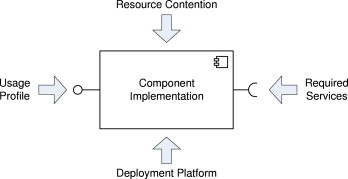
\includegraphics[width=10cm]{component-performance}
  \caption[Factores que influyen en el rendimiento de un componente]{Factores que influyen en el rendimiento de un componente. Tomado de \protect\cite{Koziolek:2010:PEC:1808359.1808729}}
  \label{fig:component-performance}
\end{figure}

\begin{itemize}
    \item \emph{Implementación del componente}: los desarrolladores pueden implementar la funcionalidad especificada en una interfaz de diferentes formas. Dos componentes pueden proporcionar el mismo servicio pero presentar tiempos de ejecución diferentes cuando se ejecutan con los mismos recursos y con las mismas entradas.
    \item \emph{Servicios requeridos}: cuando el componente $A$ invoca el servicio del componente $B$, el tiempo de ejecución de $B$ suma al tiempo de ejecución de $A$. Por lo tanto, el tiempo total de ejecución de un componente depende del tiempo de ejecución de los otros componentes/servicios que necesita.
    \item \emph{Plataforma de instalación}: los arquitectos de software instalan un componente de software en diferentes plataformas. Una plataforma de instalación puede incluir varias capas de software (como por ejemplo contenedores de componentes o máquinas virtuales) y hardware (procesador, dispositivos de almacenamiento y red, etc)
    \item \emph{Perfil de uso}: clientes pueden invocar los servicios del componente con diferentes parámetros de entrada. El tiempo de ejecución de un servicio puede cambiar dependiendo de los valores de lo parámetros de entrada.
    \item \emph{Contención de recursos}: un componente de software típicamente no se ejecuta como un solo proceso aislado en una plataforma determinada. Los tiempos de espera inducidos para acceder a recursos limitados se suman al tiempo de ejecución de un componente de software.
\end{itemize}

\subsubsection{Enfoques de ingeniería de rendimiento para software basado en componentes propuestos}
La encuesta llevada a cabo en \cite{Koziolek:2010:PEC:1808359.1808729} proporciona una clasificación de enfoques de medición y predicción de rendimiento para sistemas de software basados en componentes. Otra clasificación es la que se expone en \cite{1291833}, donde se presenta una revisión de métodos de predicción de rendimiento basado en modelos para sistemas en general, pero no analiza los requerimientos propios para sistemas basados en componentes. 

De acuerdo con \cite{Koziolek:2010:PEC:1808359.1808729} durante los últimos diez años, los investigadores han propuesto muchos enfoques para evaluar el rendimiento (tiempos de respuesta, \emph{throughput}, utlización de recursos) de sistemas de software basados en componentes. Estos enfoques abarcan tanto predicción como medición del rendimiento. Los primeros analizan el rendimiento esperado de un diseño de software basado en componentes para evitar problemas de rendimiento en la implementación del sistema, lo que podría llevar a costos substanciales para rediseñar la arquitectura. Los otros analizan el rendimiento observable de sistemas de software basados en componentes implementados para entender sus propiedades, determinar su capacidad máxima, identificar componentes críticos y para resolver cuellos de botella.

\paragraph{Métodos de evaluación de rendimiento}
Los enfoques se reunieron en dos grandes grupos: enfoques principales que proporcionan procesos de evaluación de rendimiento completo y enfoques suplementarios que se centran en aspectos específicos como medición de componentes individuales o modelaje de las propiedades de rendimiento de los conectores de un componente.

\paragraph{Enfoques principales}
\begin{itemize}
    \item \textbf{Enfoques de predicción basados en UML}: los enfoques en este grupo se enfocan en la predicción de rendimiento en tiempo de diseño para sistemas de software basado en componentes modelados con el Lenguaje de Modelado Unificado (UML por sus siglas en inglés). UML 2.0 tiene la noción de componente de software como una clase extendida. UML permite modelar el comportamiento de un componente con diagramas de secuencia, actividad y colaboración. La asignación de los componentes puede ser descrita mediante diagramas de despliegue(\emph{deployment}).     
%    Mientras que UML solamente soporta especificaciones funcionales, su mecanismo de extensión (perfiles que consisten de estereotipos, restricciones y valores etiquetados) ha sido utilizado por el \emph{Object Management Group} para permitir el modelado de atributos de rendimiento como valores de tiempo y parámetros de cargas de trabajo. 
    \begin{itemize}
        \item CB-SPE - \emph{Component-Based Software Performance Engineering} 
    \end{itemize}
    \item \textbf{Enfoques de predicción basados en Meta-Modelos propietarios}: Los enfoques en este grupo apuntan a las predicciones de rendimiento de tiempo de diseño. En lugar de usar UML como lenguaje de modelado para desarrolladores y arquitectos, estos enfoques tienen meta-modelos propietarios\cite{Koziolek:2010:PEC:1808359.1808729}.
    \begin{itemize}
        \item CBML - \emph{Component-Based Modeling Language}
        \item PECT - \emph{The Prediction Enabled Component Technology}
        \item COMQUAD - \emph{Components with Quantitative properties and Adaptivity}
        \item KLAPPER
        \item ROBOCOP
        \item Palladio        
    \end{itemize}
    \item \textbf{Enfoques de predicción centrados en \emph{middleware}}: hacen énfasis en la influencia del \emph{middleware} en el rendimiento de un sistema basado en componentes. Por lo tanto miden y modelan el rendimiento de plataformas \emph{middleware} como JavaEE o .Net. Se basan en suponer que la lógica de negocio de los componentes tiene poco impacto en el rendimiento general del sistema y por eso no requieren un modelado detallado.
    \begin{itemize}
        \item NICTA
    \end{itemize}
    \item \textbf{Enfoques basados en especificaciones formales}: estos enfoques siguen teorías fundamentales de especificación de rendimiento y no toman en cuenta marcos de trabajo (\emph{frameworks}) de medición y predicción.
    \begin{itemize}
        \item RESOLVE
        \item HAMLET
    \end{itemize}
    \item \textbf{Enfoques de monitoreo para sistemas implementados}: suponen que un sistema basado en componentes ha sido implementado y puede ser probado. El objetivo es encontrar problemas de rendimiento en un sistema en ejecución, identificar cuellos de botella y adaptar el sistema para que pueda lograr los requerimientos de rendimiento.
   \begin{itemize}
        \item COMPAS
        \item TESTEJB
        \item AQUA
        \item PAD
    \end{itemize}    
\end{itemize}
  

\paragraph{Enfoques Suplementarios}
\begin{itemize}
    \item \textbf{Enfoques de monitoreo para componentes implementados}: El objetivo de los enfoques de medición para implementaciones de componentes de software individuales es derivar especificaciones de rendimiento parametrizadas a través de mediciones múltiples. El objetivo es obtener el perfil de uso, dependencias y la plataforma de implementación a partir de la especificación de rendimiento, de modo que pueda usarse en diferentes contextos. 
    \begin{itemize}
        \item RefCAM
        \item COMAERA
        \item ByCounter
    \end{itemize}
    \item \textbf{Enfoques de predicción con énfasis en conectores de componentes}: Estos enfoques suponen un lenguaje de descripción de componentes existente y se centran en modelar y medir el impacto en el rendimiento de las conexiones entre componentes. Estas conexiones pueden implementarse con diferentes técnicas \emph{middleware}.
    \begin{itemize}
        \item Verdickt
        \item Grassi
        \item Becker
        \item Happe
    \end{itemize}        
\end{itemize}

Recientemente varios enfoques de predicción basados en meta-modelos propietarios han sido propuestos para la optimización del diseño de arquitecturas, modelado de calidad de servicio y escalabilidad. PerOpteryx\cite{Koziolek:2011:PAA:2000259.2000267} es un enfoque de optimización de diseño de arquitecturas que manipula modelos especificados en \emph{Palladio Component Model}\cite{Reussner:2016:MSS:3036121} y utiliza el algoritmo evolutivo multi-objetivo \texttt{NSGA-II}. Para análisis de rendimiento utiliza redes de colas en capas. \emph{Descartes Modeling Language}\cite{KoBrHu2014-TechReport-DML} es un lenguaje de modelado de arquitecturas para modelar calidad de servicio y aspectos relacionados con la gestión de recursos de los sistemas, las infraestructuras y los servicios de tecnología de información dinámicos modernos. \emph{CloudScale}\footnote{\url{http://www.cloudscale-project.eu/}}\cite{Brataas:2013:CSM:2479871.2479920} es un enfoque de diseño y evolución de aplicaciones y servicios escalables en la nube. En \emph{CloudScale} se identifica y gradualmente se resuelven problemas de escalabilidad en aplicaciones existentes y también permite el modelado de alternativas de diseño y el análisis del efecto de la escalabilidad en el costo. Cabe mencionar que estos últimos enfoques han sido influenciados en gran medida por el trabajo llevado a cabo en \emph{Palladio Component Model}.

\subsubsection{Modelado de Arquitecturas de Software con \emph{Palladio Component Model}} \label{sec:pcm}
El \emph{Palladio Component Model} es un enfoque de modelaje para arquitecturas de software basados en componentes que permite predicción de rendimiento basada en modelos. PCM contribuye al proceso de desarrollo de ingeniería basada en componentes y proporciona conceptos de modelaje para describir componentes de software, arquitectura de software, despliegue (\emph{deployment}) de componentes y perfiles de uso de sistemas de software basados en componentes en diferentes submodelos (Figura \ref{fig:pcm-instance}). 

\begin{figure}[h]
  \centering
  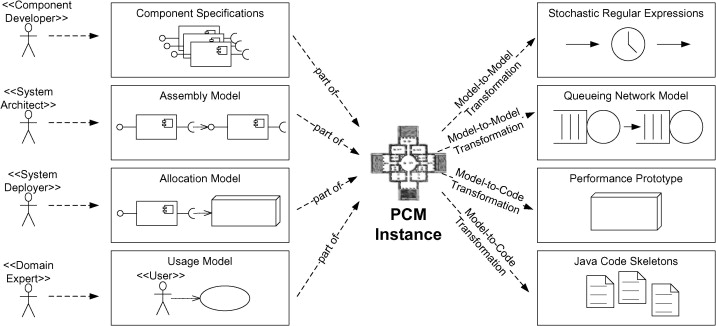
\includegraphics[width=15cm]{palladio-cbse-process}
  \caption[Instancia de un modelo PCM]{Instancia de un modelo PCM. Tomado de \protect\cite{Becker:2009:PCM:1458724.1458819}}
  \label{fig:pcm-instance}
\end{figure}

\begin{itemize}
    \item \textbf{Especificaciones de componentes} son descripciones abstractas y paramétricas de los componentes de software. En las especificaciones de software se proporciona una descripción del comportamiento interno del componente así como las demandas de sus recursos en RDSEFFs (\emph{Resource Demanding Service EFFect specifications}) utilizando una sintaxis similar a los diagramas de actividad de UML.
    \item \textbf{Un modelo de ensamblaje} (\emph{assembly model}) especifica qué tipo de componentes se utilizan en una instancia de aplicación modelada y si las instancias del componente se replican. Además, define cómo las instancias del componente se conectan, para representar la arquitectura de software.
    \item El entorno de ejecución y los recursos, así como la instalación (\emph{deployment}) de instancias de componentes para dichos contenedores de recursos se definen en un \textbf{modelo de asignación} (\emph{allocation model}).
    \item El \textbf{modelo del uso} especifica la interacción de los usuarios con el sistema utilizando una sintaxis similar al diagrama de actividades de UML, para proporcionar una descripción abstracta de la secuencia y la frecuencia con que los usuarios activan las operaciones disponibles en un sistema.
\end{itemize}

Un modelo PCM abstrae un sistema de software en el nivel de arquitectura y se anota con consumos de recursos que fueron medidos previamente y otros que son estimados. El modelo puede entonces ser usado en transformaciones de modelo-a-modelo o modelo-a-texto a un modelo de análisis en particular (redes de colas o simulación de código) que puede ser resuelto analíticamente o mediante simulación para obtener resultados sobre el rendimiento y predicciones del sistema modelado. Los resultados del rendimiento y las predicciones pueden ser utilizadas como retroalimentación para evaluar y mejorar el diseño inicial, permitiendo así una evaluación de calidad de los sistemas de software con base en un modelo\cite{Noorshams2015_1000046750}.


\subsubsection{Modelado de Arquitecturas de Software con \emph{Descartes Modeling Language}} \label{sec:dml}
El \emph{Descartes Modeling Language} (DML) es un lenguaje de modelado de nivel de arquitectura utilizado para describir calidad de servicio (\emph{QoS} por sus siglas en inglés) y aspectos relacionados con la gestión de recursos de sistemas de información dinámicos, infraestructuras y servicios. DML distingue explicítamente diferentes tipos de modelos que describen el sistema y sus procesos de adaptación desde un punto de vista técnico y lógico. Juntos, estos diferentes tipos de modelos forman una instancia DML. La idea detrás del uso de estos modelos es separar el conocimiento acerca de la arquitectura del sistema y el comportamiento de su rendimiento (aspectos técnicos), del conocimiento de los procesos de adaptación del sistema (aspectos lógicos)\cite{KoBrHu2014-TechReport-DML}.

\begin{figure}[h]
  \centering
  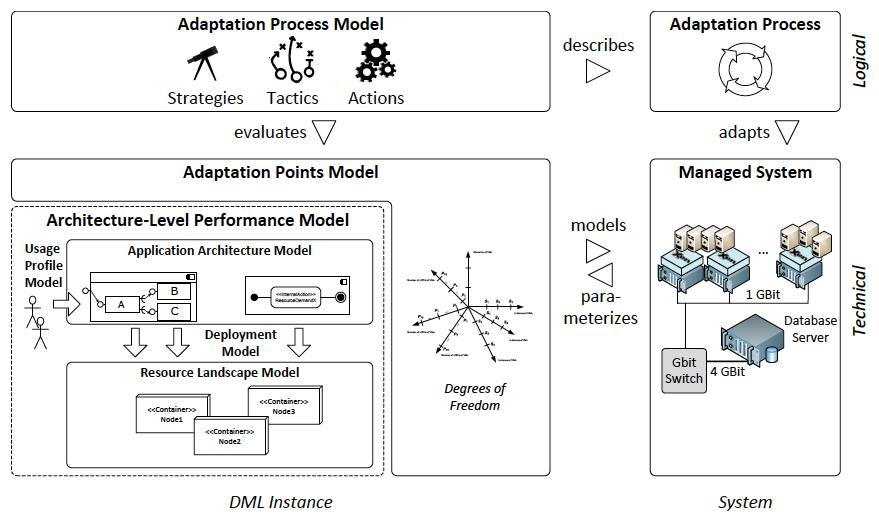
\includegraphics[width=16cm]{dml-instance}
  \caption[Relación de los diferentes modelos de una instancia DML y el sistema]{Relación de los diferentes modelos de una instancia DML y el sistema. Tomado de \protect\cite{KoBrHu2014-TechReport-DML}}
  \label{fig:dml-instance}
\end{figure}

La figura \ref{fig:dml-instance} muestra la relación de los diferentes modelos que son parte de una instancia DML, el sistema gestionado (\emph{managed system}) y el proceso de adaptación del sistema (\emph{adaptation process}). En la esquina inferior derecha de la figura \ref{fig:dml-instance}, se ve el sistema, el cual es gestionado por un proceso de adaptación, mostrado en la esquina superior derecha de la figura \ref{fig:dml-instance}. En la esquina inferior izquierda se muestran modelos que reflejan los aspectos técnicos del sistema. Esos aspectos son los recursos de hardware y su distribución (\emph{resource landscape model}), los componentes de software y el comportamiento relevante al rendimiento (\emph{application architecture model}), la instalación de componentes de software en el hardware (\emph{deployment model}), el comportamiendo del uso y las cargas de trabajo de los usuarios del sistema (\emph{usage profile model}) y los grados de libertad del sistema que pueden ser empleados para la adaptación del sistema en ejecución (\emph{adaptation points model}). Por encima de estos modelos (esquina superior izquierda de la figura \ref{fig:dml-instance}) se muestra el modelo de proceso de adaptación, que especifica un proceso de adaptación que describe cómo el sistema se adapta a cambios en su ambiente. El proceso de adaptación aprovecha las técnicas de predicción de rendimiento en línea para razonar sobre posibles estrategias, tácticas y acciones de adaptación.

\subsubsection{Enfoque de ingeniería de rendimiento declarativo}
%Las cargas de trabajo descritas en la sección \ref{sec:manejador-imagenes-spe} van a alimentar la bitácora de eventos de la función. En AWS el servicio encargado de llevar registro de los eventos que suceden en una función Lambda se llama Amazon CloudWatch\footnote{\url{https://aws.amazon.com/cloudwatch}}. 

Para obtener un modelo a partir del comportamiento de un software en existente, en Walter et al.\cite{Walter:2018:TDP:3185768.3185777} se introduce el enfoque de ingeniería de rendimiento declarativo, el cual busca la automatización de gran parte del proceso de ingeniería de rendimiento  con el fin de explorar, responder y visualizar aspectos concernientes al rendimiento de un sistema. Esto se logra gracias a una serie de herramientas desarrolladas por el grupo de ingeniería de software de la Universidad Würzburg de Alemania y que están disponibles en \url{http://descartes.tools}.

\begin{figure}[h]
  \centering
  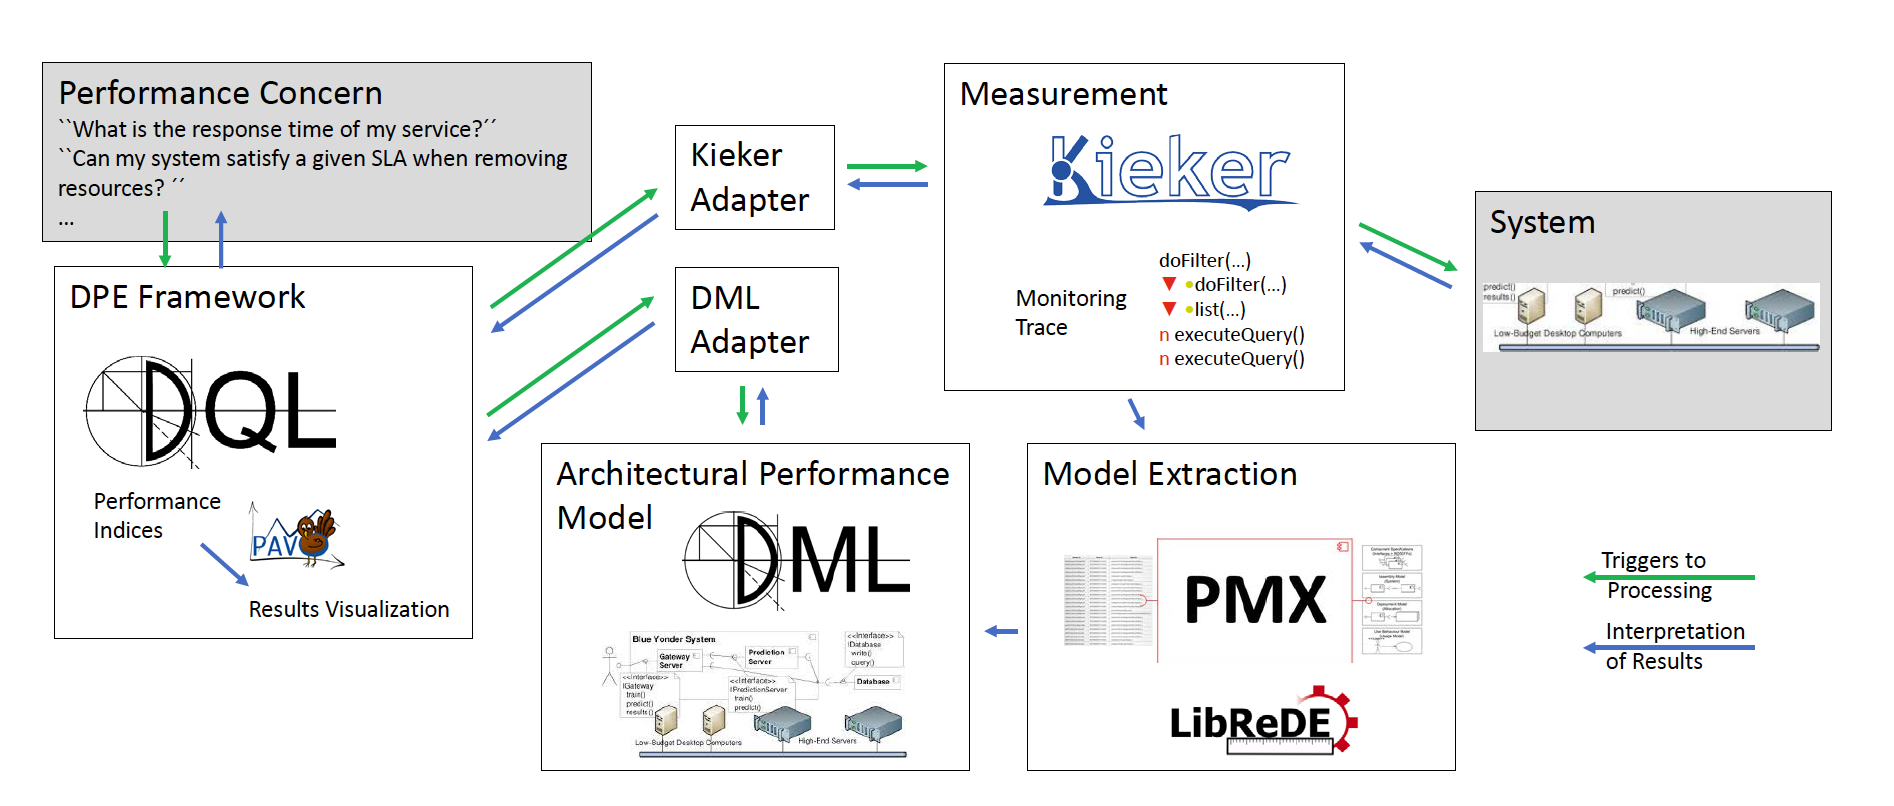
\includegraphics[width=17cm]{declarative-performance-engineering}
  \caption[Herramientas utilizadas para ingeniería de rendimiento declarativo]{Herramientas utilizadas para ingeniería de rendimiento declarativo. Tomado de \cite{Walter:2018:TDP:3185768.3185777}}
  \label{fig:declarative-performance-engineering}
\end{figure}


La figura \ref{fig:declarative-performance-engineering} muestra las herramientas involucradas en el proceso de ingeniería de rendimiento declarativo. Pueden clasificarse en: herramientas para determinar niveles de servicio, para interpretar mediciones obtenidas por medio de la ejecución de un sistema, para extraer modelos de rendimiento y para visualizar resultados. En las figura \ref{fig:declarative-performance-engineering} estas herramientas son:
\begin{itemize}
    \item \textbf{DPE Framework (DPE)}: herramienta para determinar los niveles de servicio de un sistema. Esto lo logra mediante el \emph{Descartes Query Language}(DQL), un lenguaje de consultar indicadores de rendimiento. DPE también incluye \emph{Performance Analysis Visualization} (PAVO) para la visualización de indicadores de rendimiento.
    \item \textbf{Kieker}: una herramienta para el monitoreo del rendimiento de la aplicación (APM por sus siglas en inglés). 
    \item \textbf{Performance Model Extractor (PMX)}: una herramienta que puede derivar modelos de rendimiento a partir de los datos del monitoreo del rendimiento de la aplicación. Puede tomar los datos obtenidos por Kieker y generar modelos de rendimiento en PCM y DML (sección \ref{sec:dml})
\end{itemize}

 
\subsection{Computación en nube}

Según el NIST\cite{Mell:2011:SND:2206223}, el \emph{Cloud Computing}, o la Computación en la Nube, es un modelo que, desde la perspectiva del consumidor, permite el acceso conveniente, por demanda, desde alguna red, a un conjunto de recursos computacionales específicos y configurables (por ejemplo, redes, servidores, almacenamiento, aplicaciones y servicios) que pueden ser rápidamente provisionados y entregados con un esfuerzo mínimo de administración o de interacción con el proveedor del servicio.

\subsubsection{Modelos de entrega de servicio}

La definición del NIST presenta 3 modelos básicos de servicio. Aunque los proveedores de servicios de Cloud han creado muchas variaciones de ofertas \emph{``as-a-Service''}, estos 3 siguen siendo considerados los fundamentales. En la figura \ref{fig:iaas-vs-paas-vs-saas} se muestra lo que se conoce como infraestructura como servicio (IaaS), plataforma como servicio (PaaS) y software como servicio y (SaaS) y las áreas que abarcan en términos de infraestructura, plataforma y software dentro de un esquema de computación en la nube.

\begin{figure}[h]
  \centering
  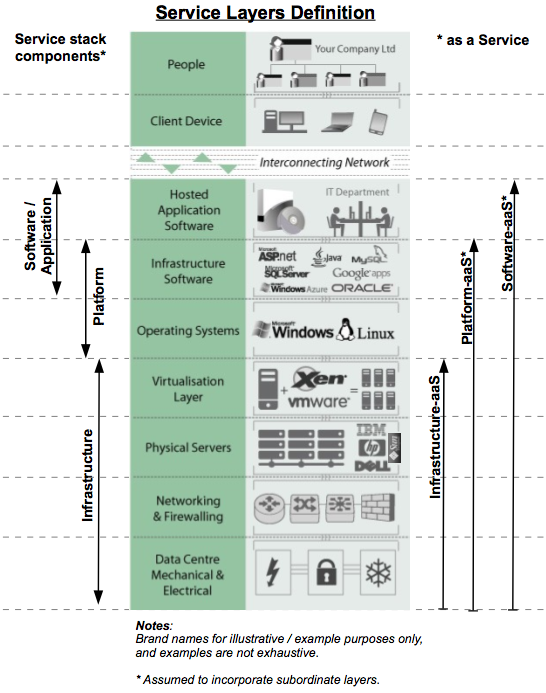
\includegraphics[width=13cm]{Kate-Service-layers-IaaS_PaaS_SaaS}
  \caption[Niveles de servicio presentes en computación en la nube]{Niveles de servicio presentes en computación en la nube. Tomado de \protect\cite{kate-craig}}
  \label{fig:iaas-vs-paas-vs-saas}
\end{figure}


\paragraph{Software como Servicio (SaaS)}
El cliente usa una aplicación, que se ofrece como un servicio accedido remotamente con protocolos estandarizados, pero no controla el sistema operativo, los servidores de aplicación, el hardware o la infraestructura de red en la que opera. El proveedor instala, administra y mantiene el software. El proveedor no necesariamente es dueño de la infraestructura física donde el software se está ejecutando. En general, se puede considerar un servicio para usuarios finales.

\paragraph{Plataforma como Servicio (PaaS)}
El cliente usa un sistema hospedado para sus aplicaciones. El cliente controla las aplicaciones que ejecuta en el ambiente (y posiblemente tenga algún control sobre el ambiente de hospedaje), pero no tiene acceso ni controla el sistema operativo, el hardware o la infraestructura de red donde ellas se ejecutan. La plataforma es típicamente un marco de ejecución aplicativo. El proveedor administra la infraestructura de software de la nube para la plataforma. En este caso, el cliente por lo general es un desarrollador de software.

\paragraph{Infraestructura como Servicio (IaaS)}
El cliente utiliza recursos computacionales fundamentales como poder de procesamiento, almacenamiento, comunicaciones y \emph{middleware}. El cliente puede controlar el sistema operativo, el almacenamiento, implementar aplicaciones y posiblemente algunos componentes de red como cortafuegos (\emph{firewalls}) y balanceadores de carga, pero la infraestructura física de red y de hardware no le pertenece. Los clientes habituales de estos servicios son administradores de sistemas.

\subsubsection{\emph{Serverless y Function-as-a-Service}}
FaaS es un área de lo que hoy se conoce como computación sin servidores o \emph{serverless computing}. Amazon.com, uno de los principales propulsores de esta tendencia define \emph{serverless} como una tecnología la cual permite construir y ejecutar aplicaciones y servicios sin necesidad de pensar en los servidores. Las aplicaciones \emph{serverless} no requieren de aprovisionamiento, escalamiento y administración de ningún servidor. Se puede construir con ella casi cualquier tipo de aplicación o servicio, y todo lo que se requiere para ejecutar y escalar la aplicación con alta disponibilidad es gestionado por el proveedor del servicio\cite{amazon:serverless-definition}. 

FaaS se refiere a un tipo de aplicación \emph{serverless} en donde la lógica del lado del servidor es escrita por un desarrollador pero, a diferencia de arquitecturas tradicionales, esta se ejecuta en contenedores de cómputo que no mantienen estado, son activados por medio de eventos, son efímeros (pueden durar solo una invocación) y son totalmente administrados por un tercero\cite{mike-roberts-serverless}.

Cabe destacar que aunque el término \emph{serverless} ha llegado a ser utilizado para referirse de forma directa a plataformas FaaS, hoy en día las aplicaciones de \emph{serverless computing} abarcan otros tipos de servicios como almacenamiento, mensajería, análisis de datos, seguridad, entre otros.

\subsubsection{Proveedores de servicios de \emph{Function-as-a-Service}} \label{sec:proveedores-faas}

Los principales proveedores de servicios de FaaS son: AWS Lambda, Google Functions, Microsoft Azure Functions e IBM Apache OpenWhisk Functions\cite{novkovic-nemanja}.

\paragraph{AWS Lambda} (\url{https://aws.amazon.com/lambda/}) Proporcionado por Amazon Web Services. Soporta varios lenguajes como NodeJS, Java, C\# y Python. Rango de asignación de memoria: mínimo 128Mb, máximo 1536Mb. Capacidad de disco (espacio en \texttt{/tmp}) 512Mb. La duración máxima de ejecución por solicitud es de 300 segundos.

El precio se establece en \$0.20 por millón de solicitudes y \$0.00001667 por Gigabyte por segundo. 1 millón de solicitudes y 400.000 GBs por mes son gratuitos.

\paragraph{Google Functions} (\url{https://cloud.google.com/functions}) Solamente soporta NodeJS. Está limitado a 1000 funciones con una duración máxima de 540 segundos por cuenta. 
El precio se establece en tres modelos diferentes. El primero es de \$ 0,40 por millón de invocaciones, pero considera que 2 millones de invocaciones son gratuitas. El segundo modelo de precio es de \$0.0000025 por GBs con 400,00 GBs por mes son gratis. El tercer modelo de precios, es de \$0.0000100 GHz por segundo con 200,000 GHz por segundo al mes que son gratuitos.

\paragraph{Microsoft Azure Functions} (\url{https://azure.microsoft.com/en-us/services/functions}) Soporta lenguajes como NodeJS, C\#, F\#, Python, PHP y Java. Azure está limitado a solo diez ejecuciones simultáneas por una función. No hay límites en el límite máximo de tiempo de ejecución. Utiliza dos modelos de precios diferentes. El primero es de \$0.000016 GBs, con 400,000 GBs por mes que son gratuitos. El segundo modelo es de \$0.20 por millón de ejecuciones, con 1 millón de ejecuciones por mes de forma gratuita.

\paragraph{IBM Apache OpenWhisk Functions} (\url{https://www.ibm.com/cloud/functions}) Soporta lenguajes como NodeJS, Swift, Java, PHP, Go y Python. Se puede utilizar cualquier otro lenguaje de programación siempre y cuando de proporcione un contenedor de Docker para esto. Tiene un costo básico que es de \$0.000017 por segundo de ejecución, por GB de memoria asignada.

\paragraph{Otros proveedores de servicios FaaS} Se pueden encontrar otros proveedores y herramientas para utilizar el modelo de funciones en la nube. Entre ellos se encuentran:
\begin{itemize}
    \item Apache OpenWhisk: \url{http://openwhisk.incubator.apache.org/}
    \item Webtask: \url{https://webtask.io/}
    \item OpenFaas: \url{https://github.com/openfaas/faas}
    \item IronFunctions: \url{https://github.com/iron-io/functions}
    \item Kubeless: \url{http://kubeless.io/}
    \item Fn Project: \url{http://fnproject.io/}
    \item Spotinst Functions: \url{https://spotinst.com/products/spotinst-functions/}
\end{itemize}

\newpage

\section{Trabajos relacionados}

\subsubsection{Ingeniería de rendimiento de software en aplicaciones en la nube}

El estilo de arquitectura basado en microservicios es uno de los que ha logrado ganar mayor adopción y popularidad dentro de la comunidad de desarrolladores. Los microservicios, son una arquitectura de software que involucra la construcción y entrega de sistemas que se caracterizan por ser servicios pequeños, granulares, independientes y colaborativos \cite{10.1007/978-3-319-62636-9_11}. Con respecto de SPE y microservicios se reporta que existen muchos retos en investigación que han sido poco o nada abordados. 

En \cite{Heinrich:2017:PEM:3053600.3053653} se planean el monitoreo, pruebas y modelado del rendimiento como las tres áreas en donde se carece de investigación y desarrollo de SPE y microservicios. Se argumenta que aún hacen falta enfoques de SPE que tomen en cuenta las particularidades de los microservicios. Aderaldo et al.\cite{7968049} señala una falta de investigación empírica repetible sobre diseño, desarrollo y evaluación de aplicaciones de microservicios y que esto dificulta la evaluación de este tipo de aplicaciones pues se cuenta con muy pocas aplicaciones y arquitecturas de referencia, así como de cargas de trabajo que contribuyan a caracterizar comportamiento.

El reporte de \cite{DBLP:journals/corr/BrunnertHWDHHHJ15} también proporciona un listado de los retos asociados con microservicios y SPE, haciendo énfasis en actividades de SPE relacionadas con la integración de actividades de desarrollo y de operaciones de puesta en producción y mantenimiento del software. Se argumenta que a pesar del alto nivel de adopción de prácticas de integración continua, entrega continua y DevOps por la comunidad de ingeniería de software, ninguna toma en cuenta aspectos relacionados con el rendimiento. Otros estudios, como el llevado a cabo en \cite{7930195}, indican que uno de los atributos de calidad que ha recibido mayor atención en la investigación en microservicios es el de la eficiencia del rendimiento pero vista mayoritariamente desde el punto de vista de la escalabilidad y mantenibilidad del código de los microservicios y su instalación.


%\textbf{[INCLUIR ESTUDIOS EN DONDE SI SE HA HECHO INVESTIGACION DE SPE Y MICROSERVICIOS?]}

\subsubsection{\emph{Serverless y Function-as-a-Service}}
%FaaS es un área de lo que hoy se conoce como computación sin servidores o \emph{serverless computing}. Amazon.com, uno de los principales propulsores de esta tendencia define \emph{serverless} como una tecnología la cual permite construir y ejecutar aplicaciones y servicios sin necesidad de pensar en los servidores. Las aplicaciones \emph{serverless} no requieren de aprovisionamiento, escalamiento y administración de ningún servidor. Se puede construir con ella casi cualquier tipo de aplicación o servicio, y todo lo que se requiere para ejecutar y escalar la aplicación con alta disponibilidad es gestionado por el proveedor del servicio\cite{amazon:serverless-definition}. 
%
%FaaS se refiere a un tipo de aplicación \emph{serverless} en donde la lógica del lado del servidor es escrita por un desarrollador pero, a diferencia de arquitecturas tradicionales, esta se ejecuta en contenedores de cómputo que no mantienen estado, son activados por medio de eventos, son efímeros (pueden durar solo una invocación) y son totalmente administrados por un tercero\cite{mike-roberts-serverless}.
%
%Cabe destacar que aunque el término \emph{serverless} ha llegado a ser utilizado para referirse de forma directa a plataformas FaaS, hoy en día la aplicaciones de \emph{serverless computing} abarcan otros tipos de servicios como almacenamiento, mensajería, análisis de datos, seguridad, entre otros.

Los investigadores han empezado a describir y analizar FaaS a través de encuestas y experimentos\cite{DBLP:journals/corr/BaldiniCCCFIMMR17,Crane:2017:ESA:3121050.3121086,8360324}, y también por análisis económicos\cite{7515686,8247460}. Sin embargo se reporta que aún no se conoce mucho acerca de SPE en FaaS. En \cite{Heinrich:2017:PEM:3053600.3053653} se menciona que al igual que con microservicios, FaaS también requiere de nuevas estrategias de modelado para capturar el comportamiento del código bajo estas infraestructuras. Los modelos de rendimiento tradicionales basados en la noción de máquinas independientes podría ser inadecuado. 

En van Eyk et al.\cite{vanEyk:2018:SRC:3185768.3186308} se presenta un informe confeccionado por el \emph{Standard Performance Evaluation Corporation RG Cloud Group\footnote{\url{https://research.spec.org/working-groups/rg-cloud.html}}} (SPEC RG Cloud) sobre desafíos asociados a rendimiento en arquitecturas FaaS. Los principales temas son los que tienen que ver con evaluación y comparación de plataformas de FaaS, reducción del \emph{overhead}, políticas de \emph{scheduling}, la relación costo-rendimiento de una función y la predicción del rendimiento. El informe también señala que actualmente muchas de las tareas de evaluación y pruebas para FaaS se vuelven complicadas porque no se cuenta con aplicaciones, arquitecturas ni cargas de trabajo de referencia; este es un trabajo que pretende abordar el SPEC RG Cloud. Con respecto a predicción del rendimiento, se indica que la aplicación de modelos de rendimiento de sistemas de software tradicionales en FaaS trae nuevos retos como la brecha de información (\emph{information gap}) y el rendimiento de una función en particular. La brecha de información significa que el usuario de FaaS no está consciente de los recursos de hardware en los que las funciones son ejecutadas, mientras que, por otro lado, la plataforma de FaaS no tiene información acerca de los detalles de la implementación de la función. Tal y como en las aplicaciones tradicionales, la entrada (tamaño, estructura y contenido) influyen en el rendimiento de una función, el hecho de tener una infraestructura oculta hace necesario encontrar nuevos modelos que logren predecir de forma precisa el rendimiento de una función. Técnicas de modelado desarrolladas para sistemas de software se podrían aprovechar para FaaS, como por ejemplo modelado y simulación de arquitecturas de software basada en componentes. 

La aplicación de \emph{serverless computing} es una área activa de desarrollo. En trabajos previos \cite{7979855,hendrickson2016serverless} se han estudiado arquitecturas alternativas de \emph{serverless computing} con el fin de explotar aspectos de rendimiento o abordar retos técnicos que otras plataformas no han hecho. También se han investigado arquitecturas para recuperación de información\cite{Crane:2017:ESA:3121050.3121086} y \emph{chatbots}\cite{Yan:2016:BCS:3007203.3007217} utilizando plataformas \emph{serverless}. Muchas otras aplicaciones se han venido desarrollando en campos como \emph{Machine Learning}, seguridad, Internet de las cosas, procesamiento de voz, sistemas de archivos, etc, y son solo una muestra del potencial de esta tecnología. Pese a este potencial, también se reporta que aún no se sabe mucho acerca de cuáles herramientas y arquitecturas tecnológicas se usan para producir, instalar y ejecutar funciones\cite{Spillner:2017:PTS:3147213.3149452}. En \cite{8360324} se examinan factores qué pueden influir en el rendimiento de plataformas de \emph{serverless computing}. De acuerdo con esto, se logran identificar cuatro estados de una infraestructura \emph{serverless}: \emph{provider cold}, \emph{VM cold}, \emph{container cold}y \emph{warm}. Además demuestra cómo el rendimiento de los servicios puede llegar a variar hasta 15 veces según estos estados.

\paragraph{Posicionamiento de la investigación con respecto de la literatura consultada}
La investigación que se propone en este documento, pretende dar un aporte al área de ingeniería de rendimiento de software en aplicaciones en la nube. De acuerdo con el material recolectado, se pudo conocer que existe una necesidad por aplicar enfoques de modelado de rendimiento en el desarrollo de sistemas modernos pero que, por otro lado, los esfuerzos que se han llevado a cabo para esto no han logrado ganar popularidad, o bien, no consideran las particularidades de la computación en la nube. Por ejemplo, se reporta que no existen enfoques de modelado de rendimiento para microservicios, el cual es hoy en día, un estilo de arquitectura de software sumamente popular.

Es por esto que se considera que la realización de un estudio exploratorio para determinar los factores que influyen en el rendimiento de una función en la nube, puede brindar nuevo conocimiento sobre cómo aplicar enfoques de ingeniería de rendimiento conocidos a estas aplicaciones y además podría representar un marco de referencia inicial por medio del cual se pueda evaluar la adopción de estas tecnologías \emph{a priori} y fundamentar el planeamiento de capacidades al dimensionar sistemas intensivos en software que vayan a usar microservicios en ambientes en la nube.


\chapter{Definición del problema}
\label{cap:problema}
De acuerdo con la revisión de la literatura, se carece de modelos de rendimiento que contribuyan a caracterizar el comportamiento de funciones en la nube alojadas en plataformas FaaS bajo distintas cargas de trabajo. Contar con tales modelos permitiría validar si las funciones en la nube pueden cumplir criterios de calidad de servicio especificados, en una consideración temprana de arquitecturas candidatas para desarrollar un sistema intensivo en software.

En las plataformas FaaS en las que se ejecutan funciones en la nube, la infraestructura tecnológica subyacente se oculta por completo de los desarrolladores y diseñadores. El conocimiento de la influencia de esta infraestructura y su configuración es vital para que los arquitectos de software puedan obtener predicciones significativas del comportamiento de una función pues, al omitirse la influencia que esta tiene, puede conducir a la generación de predicciones erróneas con respecto del rendimiento de una función. Una función que reporte tiempos de respuesta sumamente prolongados o bien la utilización de significativas cantidades de recursos puede generar grandes costos económicos y hasta llegar a ser rechazada por la plataforma FaaS.

\chapter{Justificación}
\label{cap:justificacion}
\section{Innovación}
Los aspectos más novedosos que se aportan en esta tesis son:
\begin{enumerate}
    \item Proponer un método mediante el cual se pueden obtener estimaciones del rendimiento de una función en la nube
    \item Realizar modelado y simulación basados en componentes para caracterizar el rendimiento de funciones en la nube sobre plataformas FaaS
    \item Proporcionar, a partir de lo anterior, un modelo del rendimiento de una función en la nube    
\end{enumerate}

Con respecto de (1), en \cite{vanEyk:2018:SRC:3185768.3186308} se reporta que la predicción del rendimiento es uno de los principales retos de investigación en plataformas FaaS y que no se cuenta con modelos de rendimiento que consideren las características de FaaS. Esto abre la posibilidad de explorar la aplicabilidad de técnicas conocidas de modelaje de rendimiento en sistemas de software a nuestro dominio de problema. 

(2) El modelado y simulación de arquitecturas de software basadas en componentes, representa una alternativa atractiva para abordar este problema, pues es un enfoque en donde hay una comunidad de investigación y desarrollo activa que ha logrado generar diversos tipos de herramientas para la estimación del rendimiento de sistemas informáticos. 

(3) La obtención de un modelo de rendimiento de una función en la nube (3), representaría un aporte relevante para SPE y FaaS porque significaría que existe una forma por medio de la cual evaluar el comportamiento de una función sin que esta esté necesariamente instalada en una plataforma FaaS y además permitiría que cambios futuros que necesite esa función puedan ser modelados \emph{a priori}, simularlos y obtener predicciones del impacto de los cambios.



\section{Impacto}
En distintos reportes sobre el estado de tecnologías \emph{serverless} en la industria \cite{dzone-cloud-2018,rightscale-2018,digital-ocean-2018,pivotal-june-2018} se señala que la adopción de este tipo de tecnologías va en franco aumento. En \cite{rightscale-2018} se reporta una tasa de crecimiento del 25\% en su adopción con respecto del 2017. Cloud Foundry Foundation \cite{pivotal-june-2018} indica que en el 2017 ``la mayoría'' de sus encuestados no estaban usando tecnologías \emph{serverless} mientras que para el 2018, solamente 43\% \textbf{no} lo estaba haciendo. En el informe anual del estado de tecnologías en la nube de DZone\cite{dzone-cloud-2018} se notó un incremento del 14\% con respecto del 2017 en el uso de tecnologías \emph{serverless}.

Pese a que los niveles de adopción de esta tecnología van en aumento, estos mismos reportes señalan inconvenientes tales como:
\begin{enumerate}
    \item Es necesario depender de los niveles de servicio de un proveedor
    \item Dificultad para monitorear y depurar
    \item Preocupación por parte de los desarrolladores por el ``cómo funciona'' la función en la plataforma FaaS: ¿se estarán asignando los recursos adecuados para mi función en la plataforma FaaS? ¿Cómo y cuándo se hace?
    \item Límites de tiempo de espera: dependiendo del tiempo de ejecución una función en la nube podría llegar a ser cancelada por la propia plataforma FaaS.
\end{enumerate}

Lo anterior refleja que aún existe una especie de ``área gris'' alrededor del uso de las tecnologías \emph{serverless} y en particular funciones en la nube. Esto es lo que van Eyk et al.\cite{vanEyk:2018:SRC:3185768.3186308} llama brecha de la información: el usuario de FaaS no está consciente de los recursos de hardware en los que las funciones son ejecutadas, mientras que por otro lado, la plataforma de FaaS no tiene información acerca de los detalles de la implementación de la función.

Analizar el rendimiento de una función en la nube y obtener un modelo de este contribuiría a tener un mejor entendimiento de esta tecnología y de cómo esta es gestionada por la plataforma FaaS. Esto permitiría a los arquitectos y diseñadores tener mayor control sobre los cambios en una función para que esta no solamente pueda cumplir con los requerimientos de calidad de servicio sino que también, al ser \emph{serverless} un servicio que se cobra por demanda, colaboraría a reducir gastos, ya que una función que tenga un tiempo de ejecución menor generá menores costos por el uso de la plataforma FaaS.

\section{Profundidad}
Para lograr obtener un modelo de rendimiento de una función en la nube se plantean las siguientes actividades:
\begin{itemize}
    \item Diseño e implementación de un caso de uso de referencia de una función en la nube 
    \item Obtención un modelo:
    \begin{itemize}
        \item Realizar pruebas de carga sobre la función en la nube seleccionada
        \item Obtener métricas asociadas al rendimiento a partir de bitácoras de ejecución de la función
        \item Utilizar las métricas obtenidas para suministrarlas como entrada a una herramienta de extracción de modelos de rendimiento. La herramienta generará como resultado un modelo de rendimiento
    \end{itemize}
    \item Diseñar experimentos y ejecutar simulaciones sobre el modelo obtenido, con el fin de validar las estimaciones o determinar si es necesario calibrar el modelo.
    
%     si los resultados obtenidos logran estimaciones adecuadas de la ejecución de la función o si por el contrario se necesita calibrar el modelo.
\end{itemize}

%\subsection{Implementación de un caso de uso de referencia de una función en la nube} 
%Se seleccionará un caso de uso en el cual el uso de una función en la nube haya mostrado ser una solución adecuada. Una vez identificado este caso de uso, se implementará la función y se instalará en una plataforma FaaS.

%\subsection{Obtención de un modelo} 
%Las plataformas FaaS proporcionan bitácoras en donde se registran métricas asociadas a la ejecución de la función en la nube. Se planea entonces ejecutar pruebas sobre la función en la nube bajo diferentes cargas de trabajo y de estar forma poder contar con una bitácora(s) con todas las métricas obtenidas durante el tiempo que tomó la ejecución de las pruebas. 




\chapter{Hipótesis}
\label{cap:hipotesis}
En el modelo FaaS, la infraestructura tecnológica subyacente se oculta por completo de los diseñadores y desarrolladores Asimismo, la duración de la ejecución de una función en la nube determina el costo del servicio: entre mayor sea la duración, mayor será el costo. Si bien se han realizado estudios \cite{8360324} para evaluar factores que influyen en el rendimiento de servicios basados en computación \emph{serverless}, el modelado del rendimiento de este tipo de aplicaciones se sigue presentando como un reto de investigación \cite{Heinrich:2017:PEM:3053600.3053653}. El modelado del rendimiento ha ganado considerable atención en la comunidad de ingeniería de rendimiento en las pasadas dos décadas, principalmente en sistemas de software basados en componentes \cite{Koziolek:2010:PEC:1808359.1808729}. Al finalizar y alcanzar los objetivos de la investigación se podrá contar con un marco de referencia que permitirá:
\begin{itemize}
    \item Tener una función en la nube que servirá como prueba de concepto funcional para la evaluación del rendimiento
    \item Contar un método mediante el cual se pueda analizar el rendimiento de una función en la nube por medio de modelado y simulación.
\end{itemize}


Una vez alcanzados los objetivos, será posible responder a la pregunta:


\textbf{¿Es posible estimar el rendimiento de una función en la nube por medio de modelado y simulación basados en componentes?}

\chapter{Objetivos}
\label{cap:objetivos}
\section{Objetivo general}
Diseñar un método para modelar el rendimiento de funciones en la nube alojadas en plataformas \emph{Function-as-a-Service} por medio del modelado y la simulación basados en componentes, con el fin de evaluar los factores que pueden influir en su comportamiento. 

\section{Objetivos específicos}
\begin{enumerate}
    \item Revisar el estado del arte de trabajos relacionados con enfoques de predicción y medición del rendimiento en sistemas de software como servicio.
    \item Sintetizar un caso de uso de una función en la nube considerada como de referencia, con el propósito de analizar su comportamiento.
    \item Elaborar, conforme a un diseño experimental, pruebas de rendimiento sobre el caso de uso seleccionado a fin de obtener datos base.
    \item Analizar los datos experimentales mediante herramientas de extracción de modelos de rendimiento de software.
    \item Proponer y validar modelos de rendimiento a partir de los experimentos realizados.        
    \item Formular una guía metodológica para dar a conocer aspectos de rendimiento en funciones en la nube a partir de la experiencia obtenida.
\end{enumerate}

\chapter{Entregables}
\label{cap:entregables}
\section[Revisión de literatura]{Revisión de literatura\\\small{Alineado con objetivo específico 1}}
Se pretende identificar los resultados de otros estudios relacionados con el modelado de rendimiento de software, así como retos y oportunidades de investigación que existan en esta área. Las preguntas de investigación inicialmente propuestas son las siguientes:
\begin{itemize}
    \item[\textbf{PI1}] ¿Cuáles enfoques de predicción y medición del rendimiento en sistemas de software basados en componente se han propuesto?
    \item[\textbf{PI2}] ¿Cuáles enfoques de predicción y medición de rendimiento de software se han utilizado para aplicaciones en la nube?
    \item[\textbf{PI3}] ¿Qué retos y oportunidades existen con estos enfoques en la actualidad?
    \item[\textbf{PI4}] ¿Qué herramientas hay disponibles para el modelado de rendimiento de software?
\end{itemize}

\section[Implementación de caso de uso de función en la nube]{Implementación de un caso de uso de función en la nube\\\small{Alineado con objetivo específico 2}}

Identificar un caso de uso de que sea considerado como de referencia o de utilidad común en donde las funciones en la nube hayan mostrado ser un buenas candidatas para su solución. Se procederá a implementar este caso de uso e instalarlo en una plataforma FaaS. Esta será la función que servirá como base para futuros análisis.

\section[Pruebas sobre el caso de uso]{Pruebas sobre el caso de uso\\\small{Alineado con objetivo específico 3}}

\subsection{Diseño experimental}
Planeamiento y definición de las variables por observar de las pruebas de carga.

\subsection{Pruebas de carga}
Diseño, ejecución y análisis de los resultados de las pruebas.

\newpage

%\subsection{Resultados}


%\section[Medición del rendimiento del caso de uso]{Medición del rendimiento del caso de uso\\\small{Alineado con objetivo específico 3}}
%Al caso de uso identificado se le realizarán mediciones de su rendimiento por medio de diferentes cargas de trabajo. Esto permitirá conocer el comportamiento de la función y utilizar los resultados obtenidos en estas mediciones para contrastar resultados posteriores.

\section[Modelado y análisis del rendimiento de la función]{Modelado y análisis del rendimiento de la función\\\small{Alineado con objetivo específico 4}}
Se tomarán los datos generados por las pruebas anteriores para utilizarlas como entrada y, a partir de ellos, realizar una labor de análisis y modelado.

\section[Modelo de rendimiento de la función en la nube]{Modelo de rendimiento de la función en la nube\\\small{Alineado con objetivo específico 5}}
A partir de la función propuesta, pruebas y análisis del rendimiento por medio de herramientas de modelado, se propondrá un modelo que logre caracterizar el comportamiento de la función.

\subsection[Simulaciones sobre el modelo propuesto]{Simulaciones sobre el modelo propuesto}
Para validar el modelo propuesto, se ejecutarán simulaciones sobre él y de esta forma determinar si los resultados de las simulaciones se corresponden con los obtenidos en las pruebas de rendimiento de la función.

\section[Guía metodológica]{Guía metodológica\\\small{Alineado con objetivo específico 6}}
Una vez realizado el estudio, se estructurará una descripción del método utilizado para estimar el rendimiento de una función en la nube. 

\chapter[Implementación de una \emph{FaaS}: manejador de imágnenes]{Implementación de una función en la nube: manejador de imágenes}
\label{cap:manejador-imagenes}
Uno de los principales problemas de hacer ingeniería de rendimiento para software en la nube es que no existen aplicaciones de referencia que hayan ganado popularidad o cuyo desarrollo se encuentre activo. A pesar de esto y de su reciente adopción, la industria ha empezado a reconocer casos de uso en donde las aplicaciones \emph{serverless} encajan mejor. Amazon Web Services(AWS)\cite{serverless-architecture-patterns} reconoce cinco patrones de uso predominantes en su servicio AWS Lambda:
\begin{enumerate}
    \item Procesamiento de datos dirigidos por eventos.
    \item Aplicaciones Web.
    \item Aplicaciones móviles e Internet las cosas (IoT).
    \item Ecosistemas de aplicaciones \emph{serverless}.
    \item Flujos de trabajo dirigidos por eventos.
\end{enumerate}
 
Uno de las aplicaciones más comunes en \emph{serverless} es desencadenar acciones luego de que ocurre un evento (1), por ejemplo después de la modificación de un registro en una base de datos o bien luego de que se publica un mensaje en una cola de mensajería. Esto puede provocar que se active una función Lambda\footnote{En la plataforma AWS Lambda } que toma como entrada el evento recién publicado para su posterior procesamiento. Este estilo de caso de uso encaja bien en ambientes híbridos: ambientes en donde tecnologías \emph{serverless} se aprovechan para realizar funciones específicas dentro de una aplicación (o aplicaciones) más grande(s).

AWS ha publicado una serie de arquitecturas de referencia\cite{aws-lambda-ref-arch} para su plataforma FaaS, AWS Lambda. Dentro de estas arquitecturas se destaca el caso de uso de un manejador de imágenes (\emph{Image Handler})\cite{aws-lambda-image-handler}. 

\begin{figure}[h]
  \centering
  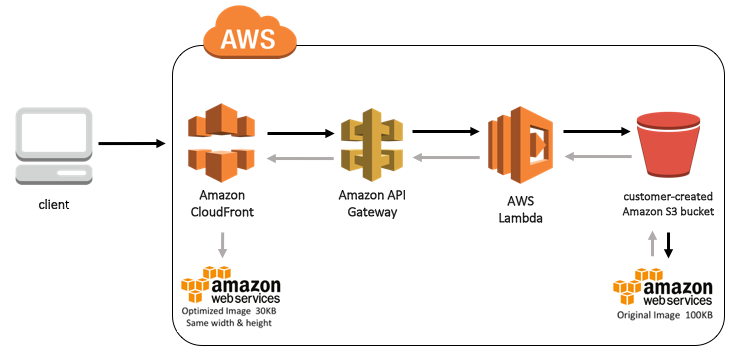
\includegraphics[width=15cm]{serverless-image-handler-architecture}
  \caption[Arquitectura del manejador de imágenes]{Arquitectura del manejador de imágenes. Tomado de \protect\cite{aws-lambda-image-handler}}
  \label{fig:serverless-image-handler-architecture}
\end{figure}

\section{\emph{Manejador de imágenes}} \label{sec:manejador-imagenes-1}
Los sitios Web con imágenes grandes pueden experimentar tiempos de carga prolongados, es por esto que los desarrolladores proporcionan diferentes versiones de cada imagen para que se acomoden a distintos anchos de banda o diseños de página. A fin de brindar tiempos de respuesta cortos y disminuir el costo de la optimización, manipulación y procesamiento de las imágenes, AWS propone un manejador de imágenes \emph{serverless}, al cual se le puedan delegar trabajos tales como una función Lambda sobre la plataforma FaaS.


A continuación se describe la arquitectura de la figura \ref{fig:serverless-image-handler-architecture}:
\begin{enumerate}
    \item Amazon CloudFront provee una capa de \emph{cache} para reducir el costo del procesamiento de la imagen
    \item Amazon API Gateway brinda acceso por medio de HTTP a las funciones Lambda
    \item AWS Lambda obtiene la imagen de un repositorio de Amazon Simple Storage Service (Amazon S3) y, por medio de la implementación de la función se retorna una versión modificada de la imagen al API Gateway
    \item El API Gateway retorna una nueva imagen a CloudFront para su posterior entrega a los usuarios finales
\end{enumerate}

Cabe mencionar que, en este contexto, una versión modificada de una imagen será cualquier imagen que haya presentado algún tipo de alteración con respecto de una imagen original como, por ejemplo, cambios de tamaño, color, metadatos, etc.

\subsection{Manejador de imágenes para SPE} \label{sec:manejador-imagenes-spe}
Para este estudio se proponemos implementar una variación del manejador de imágenes de la sección \ref{sec:manejador-imagenes-1}, que se muestra en la figura \ref{fig:serverless-image-handler-architecture-spe}.

\begin{figure}[h]
  \centering
  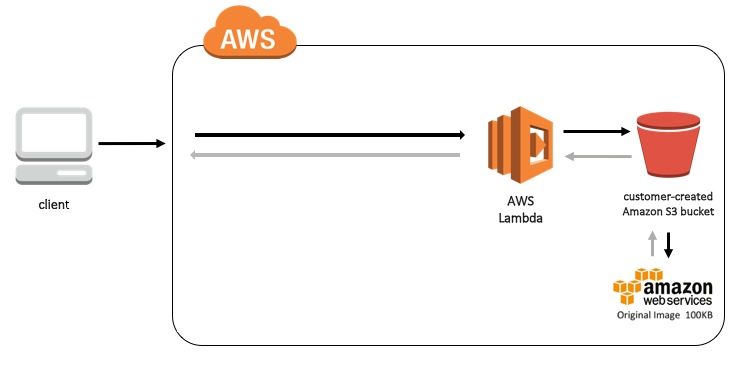
\includegraphics[width=15cm]{serverless-image-handler-architecture-spe}
  \caption[Arquitectura del manejador de imágenes propuesto para el estudio]{Arquitectura del manejador de imágenes propuesto para el estudio. Elaboración propia.}
  \label{fig:serverless-image-handler-architecture-spe}
\end{figure}

Se han dejado por fuera intencionalmente el AWS CloudFront y el AWS API Gateway. La razón de esto es porque se pretende ejercitar la función Lambda directamente. Se implementará una función Lambda que entregue, a partir de una solicitud de redimensionamiento de una imagen almacenada, otra con dimensiones diferentes producida ``al vuelo'' como respuesta a la solicitud. Por ejemplo, si la imagen original mide 500 pixeles de ancho y alto, entregar una con dimensiones de 100 pixeles de ancho y alto. 

Las actividades involucradas en el proceso de redimensionamientos de imágenes se muestran en la figura \ref{fig:serverless-image-handler-architecture-workflow}
\begin{enumerate}
    \item Se envía una solicitud de redimensionamiento de imagen en formato \texttt{JSON} a la función Lambda con los datos acerca de la localización de la imagen y su nuevo tamaño.
    \item La solicitud de redimensionamiento llega a la función Lambda.
    \item La función Lambda solicita al servicio de almacenamiento AWS S3 la imagen.
    \item AWS S3 entrega a la función Lambda la imagen solicitada.
    \item La función Lambda inicia el redimensionamiento de la imagen de acuerdo a los parámetros solicitados.
    \item La nueva imagen modificada se entrega al cliente(s).
\end{enumerate}

\begin{figure}[h]
  \centering
  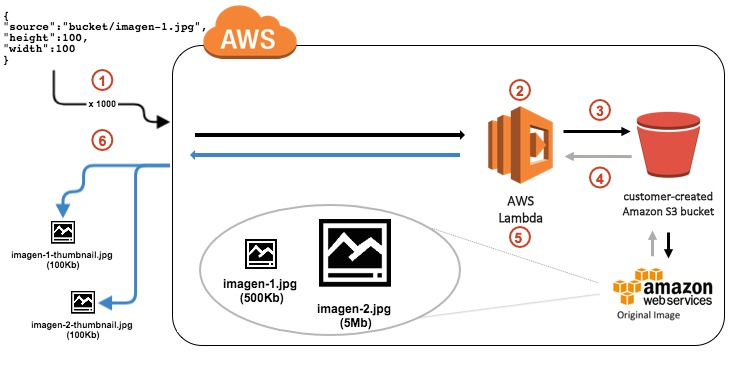
\includegraphics[width=17cm]{serverless-image-handler-architecture-workflow-2}
  \caption[Carga de trabajo sugerida para el manejador de imágenes]{Carga de trabajo sugerida para el manejador de imágenes. Elaboración propia.}
  \label{fig:serverless-image-handler-architecture-workflow}
\end{figure}


A la función Lambda se le realizarán pruebas con imágenes de entrada de distinto tamaño y cargas de trabajo variables para evaluar su comportamiento bajo estos escenarios. Se desea observar el impacto de las pruebas en el tiempo de respuesta de la función. Los resultados obtenidos a partir de estas pruebas van a servir como un punto de referencia para experimentos futuros, como los que se indican en la Sección \ref{cap:diseno-experimental}. La figura \ref{fig:serverless-image-handler-architecture-workflow} muestra una sugerencia de dos posibles cargas de trabajo: 

\begin{enumerate}
    \item 100 solicitudes de cambio de tamaño de una imagen grande. En la figura \ref{fig:serverless-image-handler-architecture-workflow}, \texttt{imagen-2.jpg} de tamaño de 5Mb, representa una imagen grande.
    \item 100 solicitudes de cambio de tamaño de una imagen pequeña. En la figura \ref{fig:serverless-image-handler-architecture-workflow}, \texttt{imagen-1.jpg} de tamaño menor o igual a 500Kb, representa una imagen pequeña.
\end{enumerate}

En principio las cargas de trabajo generadas serían \emph{cerradas}, lo que quiere decir que una solicitud se ejecuta solamente hasta que la anterior se termina. Esto ayudará en principio a tener mejor trazabilidad de lo que ocurre con la función. Cargas de trabajo separadas y secuenciales facilitan el control de los experimentos y el análisis de datos.

\paragraph{¿Por qué este caso de uso se considera relevante?}
A continuación se listan las características que hacen este caso de uso representativo e interesante:
\begin{itemize}
    \item Sencillo de entender e implementar: se cuenta únicamente con una función la cual lleva a cabo una tarea muy específica.
    \item Popular: sigue un patrón de procesamiento dirigido por eventos y, como se señala en \cite{serverless-architecture-patterns}, este es uno de los más populares que se ha empezado a adoptar para aplicaciones \emph{serverless}. Otra de las razones de la popularidad de este caso de uso es que permite a los desarrolladores crear una unidad de instalación independiente y especializada para el manejo de imágenes, liberando así a sus servidores y aplicaciones del manejo de las peticiones y, la lógica asociadas a estas.
    \item Replicable en otros proveedores de servicios en la nube: varias de las arquitecturas de referencia para \emph{serverless} propuestas por Amazon, están compuestas por herramientas y servicios muy propios de su plataforma, lo cual hace muy difícil su reproducibilidad utilizando otros proveedores. Aunque en principio este trabajo plantea ser elaborado en la plataforma FaaS de Amazon Web Services, AWS Lambda, otros proveedores de servicios (ver sección \ref{sec:proveedores-faas}) en la nube cuentan con sus propias plataformas de FaaS y de almacenamiento, lo cual permitiría replicar lo aquí propuesto en ellos.
    \item Replicable en los lenguajes de programación soportados por plataformas FaaS: actualmente JavaScript, Java (y lenguajes basados en la \emph{Java Virtual Machine}), Python, C\# y Go son los principales lenguajes de programación soportados por las plataformas FaaS. El caso de uso propuesto, no presenta ningún tipo de característica que lo ate a un lenguaje de programación en particular. La mayoría de los lenguajes de programación cuentan con bibliotecas para procesamiento de imágenes tanto de forma nativa como por medio de soluciones de terceros. Por ejemplo, en Java, se cuenta con: Java2D, \emph{imgscalr} \footnote{\url{https://github.com/rkalla/imgscalr}}, \emph{thumbnailator}\footnote{\url{https://github.com/coobird/thumbnailator}}, entre otras.
\end{itemize}


\section{Implementación del \emph{manejador de imágenes}}
Existen soluciones disponibles que se pueden estudiar para implementar un manejador de imágenes. Amazon proporciona dos ejemplos que siguen la arquitectura de la figura \ref{fig:serverless-image-handler-architecture}:
\begin{enumerate}
    \item \textbf{{serverless-image-resizing}}\footnote{\url{https://github.com/amazon-archives/serverless-image-resizing}}: escrita en lenguaje JavaScript. Utiliza el modulo \emph{sharp}\footnote{\url{https://github.com/lovell/sharp}} de NodeJS para aplicar operaciones de conversión en imágenes tales como redimensionamiento, rotación y corrección gamma.
    \item \textbf{{serverless-image-handler}}\footnote{\url{https://github.com/awslabs/serverless-image-handler}}: escrita en lenguaje Python. Hace uso del paquete \emph{Thumbor}\footnote{\url{http://thumbor.org}} de código abierto para realizar operaciones de redimensionamiento, rotación, recorte y aplicación de filtros en imágenes.
\end{enumerate}

A pesar que Amazon recomienda el uso de \emph{serverless-image-handler} sobre \emph{serverless-image-resizing}, ambas soluciones siguen un patrón sumamente similar en su codificación e instalación. 

Otro ejemplo de una función en la nube encargada de ofrecer un servicio de redimensionamiento en imágenes, es la \emph{Course\_LambdaResizer}, una función lambda usada como referencia en el curso \emph{``Serverless API on AWS for Java developers''} ofrecido en el sitio Web Udemy\footnote{\url{https://www.udemy.com/serverless-api-aws-lambda-for-java-developers}}. Esta función está escrita en lenguaje Java y utiliza la biblioteca \emph{imgscalr} para redimensionar imágenes.

Para este estudio, se implementó una función escrita en lenguaje Java. Esto motivado principalmente por la compatibilidad de este lenguaje con las herramientas para monitoreo de aplicaciones y extracción de modelos de rendimiento, Kieker y PMX respectivamente.

\subsection{Función Lambda: \emph{Image-Handler} (IM-Simple)}\label{sec:image-handler}
La función Lambda creada para este estudio lleva por nombre \emph{Image-Handler}. El código fuente y documentación relacionada con ella se encuentra disponible en GitHub.com, en el repositorio de código: \url{https://github.com/seminario-dos/image-handler}. El punto de entrada de la función Lambda es la clase \texttt{ImageHandler.java}. Esta función se encarga de realizar tres operaciones para procesar una solicitud de redimensionamiento de imagen:

\begin{enumerate}
    \item Procesar la solicitud de redimensionamiento (la entrada) que viene dada en formato JSON. Esta solicitud de redimensionamiento contiene entre otras cosas:
    \begin{itemize}
        \item El nombre de la imagen original que reside en el servicio Amazon S3.
        \item Los parámetros de altura y ancho a los que se desea redimensionar la imagen original.
    \end{itemize}
    \item Obtener la imagen del servicio Amazon S3 y posteriormente aplicarle la operación de redimensionamiento de acuerdo con los parámetros de altura y ancho especificados en la solicitud de redimensionamiento.
    \item Tomar la imagen redimensionada, codificarla en \texttt{Base64} y escribir el resultado en el flujo(\emph{stream}) de salida de la función Lambda.
\end{enumerate}
 
Un extracto de la clase \texttt{ImageHandler.java} se muestra en el listado \ref{lst:lambda-1}. En la línea \texttt{22} se procesa el evento de entrada que viene dado en formato JSON. Como resultado de esto se entrega un objeto \texttt{ImageRequest}, el cual contiene la información de la solicitud de la imagen que se desea redimensionar y que se encuentra alojada en el servicio Amazon S3.

En la línea \texttt{24} se llama al servicio \texttt{ImageService} con el fin de obtener la imagen   original (de acuerdo con la información presente en el \texttt{ImageRequest} proporcionado) y se aplica la operación de redimensionamiento.

Por último, en la línea \texttt{26}, \texttt{ImageHandlerResponseWriter.writeResponse()} toma la nueva imagen, con nuevas dimensiones de alto y ancho, la codifica en \texttt{Base64} y escribe el resultado en el \emph{stream} de salida de la función. 

\renewcommand\lstlistingname{Listado}
\begin{lstlisting}[linewidth=16.5cm, caption={Clase \texttt{ImageHandler.java}}, label={lst:lambda-1}]
public class ImageHandler implements RequestStreamHandler {

    private static final AppConfig APP_CONFIG;
    private final AppConfig appConfig;

    static {
        APP_CONFIG = AppConfig.getInstance();
    }

    public ImageHandler() {
        this(APP_CONFIG);
    }

    public ImageHandler(AppConfig appConfig) {
        this.appConfig = appConfig;
    }

    @Override
    public void handleRequest(InputStream inputStream, 
                              OutputStream outputStream, 
                              Context context) throws IOException {
        ImageRequest imageRequest = 
            this.inputEventParser().processInputEvent(inputStream);
        InputStream imageResized = 
            this.imageService().getImageFrom(imageRequest);
        this.imageHandlerResponseWriter()
            .writeResponse(imageResized, outputStream, imageRequest);
    }

    private InputEventParser inputEventParser() {
        return this.appConfig.getInputEventParser();
    }

    private ImageService imageService() {
        return this.appConfig.getImageService();
    }

    private ImageHandlerResponseWriter imageHandlerResponseWriter() {
        return this.appConfig.getImageHandlerResponseWriter();
    }
}    
\end{lstlisting}


Las funciones Lambda en AWS reciben como entrada un objeto JSON. Este objeto puede contener distintos campos dependiendo del servicio que haya invocado previamente la ejecución de la función Lambda. Debido a que la función \emph{Image-Handler} pretende ser invocada por medio de solicitudes \texttt{HTTP}, esta se configuró para que trabajara en conjunto con el servicio \texttt{API Gateway}. Dentro de este servicio se creó un recurso Web que entrega solicitudes de tipo \texttt{HTTP GET} a la función Lambda para su posterior procesamiento.

En términos generales, cada vez que una solicitud \texttt{HTTP GET} ingresa al \texttt{API Gateway} con el siguiente formato:\\ \texttt{https://\{host\}/image/\{image\}?width=\{value\}\&height=\{value\}}\\ se tomarán el nombre de la imagen original que viene en el parámetro \texttt{image} y los parámetros de ancho y alto, \texttt{width} y \texttt{height} respectivamente, y se pasarán como parámetros de entrada a la función Lambda como parte de un objeto JSON. Este objeto JSON contiene otros campos que dan a conocer a la función Lambda información acerca de la solicitud \texttt{HTTP}.

\paragraph{Ejemplo:} para la siguiente solicitud \texttt{HTTP}:
\begin{verbatim}
GET https://{host}/images/original-pic.jpg?width=50&height=66
\end{verbatim}

\noindent \texttt{API Gateway} produce el objeto JSON listado en \ref{lst:lambda-api-gateway-input}. A pesar que el objeto JSON incluye otros campos, para efectos del \emph{Image-Handler} solamente tres de ellos serán utilizados:
\begin{enumerate}
    \item \texttt{pathParameters}: contiene el nombre de la imagen original a ser redimensionada.
    \item \texttt{isBase64Encoded}: señala si la solicitud necesita ser codificada en \texttt{Base64} o no. 
    \item \texttt{queryStringParameters}: bajo esta propiedad se listan los parámetros de ancho(\texttt{width}) y alto(\texttt{height}).
\end{enumerate}


\begin{lstlisting}[caption={Clase \texttt{ImageHandler.java}}, label={lst:lambda-api-gateway-input}]
{
  "headers": {
    "Accept": "*/*",
    "User-Agent": "HTTPie/1.0.2",
    "Connection": "keep-alive",
    "X-Forwarded-Proto": "http",
    "Host": "localhost:3000",
    "Accept-Encoding": "gzip, deflate",
    "X-Forwarded-Port": "3000"
  },
  "pathParameters": {
    "image": "original-pic.jpg"
  },
  "path": "/images/original-pic.jpg",
  "isBase64Encoded": true,
  "requestContext": {
    "accountId": "123456789012",
    "path": "/images/{image+}",
    "resourceId": "123456",
    "stage": "prod",
    "requestId": "c6af9ac6-7b61-11e6-9a41-93e8deadbeef",
    "identity": {
      "cognitoIdentityPoolId": null,
      "accountId": null,
      "caller": null,
      "apiKey": null,
      "sourceIp": "127.0.0.1",
      "cognitoAuthenticationType": null,
      "cognitoAuthenticationProvider": null,
      "userArn": null,
      "userAgent": "Custom User Agent String",
      "user": null
    },
    "resourcePath": "/images/{image+}",
    "httpMethod": "GET",
    "extendedRequestId": null,
    "apiId": "1234567890"
  },
  "resource": "/images/{image+}",
  "httpMethod": "GET",
  "body": null,
  "queryStringParameters": {
    "width": "50",
    "height": "66"
  },
  "stageVariables": null
}
\end{lstlisting}

\subsubsection{Principales interacciones dentro de \emph{Image-Handler}}
La figura \ref{fig:secuencia-image-handler} muestra las principales interacciones que lleva a cabo la función \emph{Image-Handler}. Tanto las acciones como los actores involucrados, concuerdan con lo descrito en la Sección \ref{sec:image-handler} aunque, a diferencia de lo descrito allí, aquí se presenta la clase \texttt{S3Dao} que es la que se encarga de buscar y traer la imagen original del servicio Amazon S3. 
\begin{figure}[h]
  \centering
  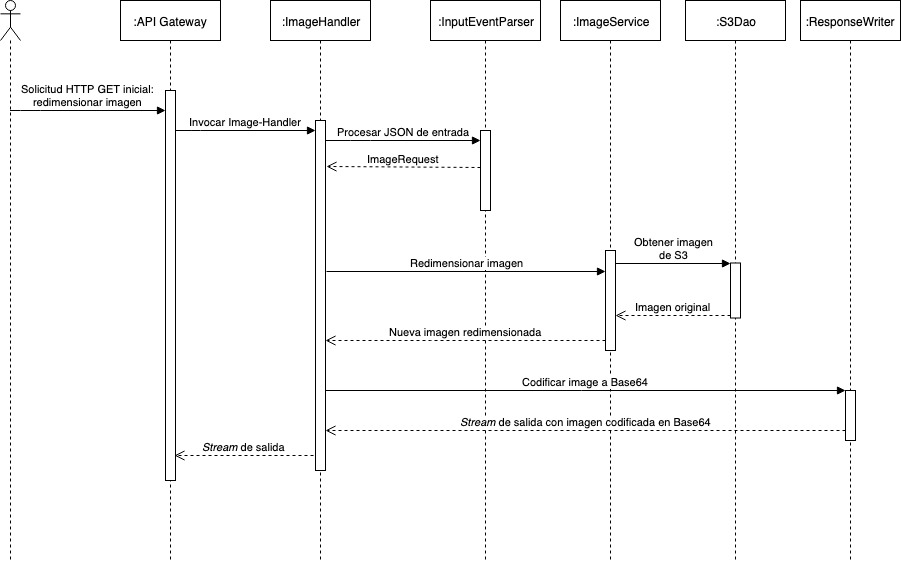
\includegraphics[width=16.5cm]{secuencia-image-handler}
  \caption[Secuencia de acciones llevadas a cabo por \emph{Image-Handler}]{Secuencia de acciones llevadas a cabo por \emph{Image-Handler}. Elaboración propia.}
  \label{fig:secuencia-image-handler}
\end{figure}

\subsection{Versiones alternas de \emph{Image-Handler}}

Aparte de la versión original de \emph{Image-Handler}, se crearon dos versiones alternas con el fin de instrumentalizar el código fuente para la extracción y generación de un modelo en PCM y, para la obtención de mediciones del rendimiento. 

En la primera version, el código se modificó para generar rastros del rendimiento de la función Lambda y extraer a partir de estos un modelo de rendimiento en PCM. La segunda versión fue modificada para generar rastros de rendimiento pero, a diferencia de la versión anterior, los datos obtenidos en esta versión fueron de mayor utilidad para afinar las estimaciones de rendimiento de los componentes involucrados en la función.

\subsubsection{Versión instrumentalizada para Kieker y PMX (IM-KP)} \label{sec:image-handler-kieker-pmx}

Uno de los principales objetivos de este trabajo es el de obtener un modelo de rendimiento a partir 
del código en ejecución de una función en la nube. Aunque el modelo de rendimiento puede ser creado por los diseñadores e implementadores sin necesidad de una herramienta que ayude a su extracción, el uso de una herramienta especializada para esto contribuye a la generación sistemática de un modelo objetivo que pueda incluir mayores niveles de detalle en cuanto a la estructura y las estimaciones del comportamiento de un artefacto de software. Además, debido a que se están dando los primeros pasos en el campo del modelado y la simulación de rendimiento basado en componentes, es preferible delegar tareas de extracción y estimaciones a herramienta(s), con el fin de aprender de lo resultados obtenidos e ir introduciendo cambios paulatinamente; la creación manual de modelos de rendimiento puede llegar a ser muy compleja, consumir mucho tiempo y está propensa a errores. 

Para lograr esto, se seleccionaron dos herramientas, Kieker y PMX, las cuales en conjunto proporcionan un marco de trabajo por medio del cual se puede obtener mediciones del rendimiento de una aplicación y luego, a partir de estas, extraer un modelo de rendimiento basado en PCM. La selección de estas herramientas y el enfoque de medición y extracción de modelos de rendimiento se seleccionó luego de estudiar el \emph{enfoque de ingeniería de rendimiento declarativo} propuesto en \cite{Walter:2018:TDP:3185768.3185777}.


%Kieker se utiliza para el estudiar el comportamiento del rendimiento del sistema a partir de las entradas/rastros que se registran en una bitácora. Creada y mantenida por el grupo de ingeniería de software de la Universidad de Kiel en conjunto con el grupo de sistemas de software de la Universidad de Stuttgart, Kieker se define como una herramienta para monitoreo del rendimiento y análisis dinámico de aplicaciones y se desarolló como parte de las actividades de enseñanza e investigación de ambas universidades. Otras instituciones académicas y de la industria también han realizado contribuciones.

Kieker se utiliza para el estudiar el comportamiento del rendimiento del sistema a partir de las entradas/rastros que se registran en una bitácora. Kieker ofrece adaptadores de monitoreo (\emph{monitoring adapters}) escritos en lenguaje Java (también ofrece adaptadores en otros lenguajes). Los dos principales componentes de Kieker son: \texttt{Kieker.Monitoring} y \texttt{Kieker.Analysis}. \texttt{Kieker.Monitoring} es el responsable de la instrumentación del código, recolección de datos y registro(\emph{logging}). El componente \texttt{Kieker.Analysis} es el responsable de leer, analizar y visualizar los datos monitoreados.

En esta versión de \emph{Image-Handler} se modificó el código original para generar registros del rendimiento de la ejecución de la función utilizando las bibliotecas proporcionadas por Kieker, utilizando como referencia lo especificado en el manual de usuario de Kieker\cite{kieker-user-guide}. Se crean objetos de tipo \texttt{OperationExecutionRecord} los cuales contienen la información acerca del rendimiento de una invocación sobre alguna parte del código.  En el listado \ref{lst:image-handler-kieker} se puede ver un extracto del código de la función instrumentalizada para que genere objetos\\ \texttt{OperationExecutionRecord}.

Adicionalmente se configuró la biblioteca para que publique los objetos\\ \texttt{OperationExecutionRecord} a modo eventos a una cola de mensajería \emph{Java Message Service} (JMS), en lugar de una bitácora local.

\begin{minipage}[c]{\linewidth}
\begin{lstlisting}[caption={Extracto de la clase \texttt{ImageHandler.java} instrumentalizada con Kieker}, label={lst:image-handler-kieker}]
public class ImageHandlerKieker implements RequestStreamHandler {
    private static final IMonitoringController MONITORING_CONTROLLER;
    static {
        MONITORING_CONTROLLER = MonitoringController.getInstance();
    }
    .
    .
    .
    
    @Override
    public void handleRequest(InputStream inputStream, OutputStream outputStream, Context context) throws IOException {

        final long tin = MONITORING_CONTROLLER.getTimeSource().getTime();
        handleRequestInternal(inputStream, outputStream, context);
        final long tout = MONITORING_CONTROLLER.getTimeSource().getTime();
        final OperationExecutionRecord e = new OperationExecutionRecord("public void "+ this.getClass().getName()+".handleRequest(InputStream, OutputStream, Context)",
                OperationExecutionRecord.NO_SESSION_ID,
                OperationExecutionRecord.NO_TRACE_ID,
                tin, tout,
                InetAddress.getLocalHost().getHostName(),
                0,
                0);
        MONITORING_CONTROLLER.newMonitoringRecord(e);
    }
    .
    .
    .
}    
\end{lstlisting}
\end{minipage}

\emph{Performance Model Extractor} (PMX), es una herramienta que automatiza la extracción de modelos de rendimiento a partir de mediciones. PMX utiliza como entrada las bitácoras basadas en Kieker y es capaz de crear modelos basados en \emph{Palladio Component Model} a partir de estas. 

%Esta es una herramienta creada y mantenida por el grupo de ingeniería de software de la Universidad Würzburg en Alemania.

%En conjunto, Kieker y PMX, proporcionan un marco de trabajo por medio del cual se puede obtener mediciones del rendimiento de una aplicación y luego, a partir de estas, extraer un modelo de rendimiento basado en PCM. La selección de estas herramientas y el enfoque de medición y extracción de modelos de rendimiento se seleccionó luego de estudiar el \emph{enfoque de ingeniería de rendimiento declarativo} propuesto en \cite{Walter:2018:TDP:3185768.3185777}.
%
%Esta versión de \emph{Image-Handler} fue la que se utilizó para obtener un modelo de rendimiento en \emph{Palladio Component Model} a partir de la bitácora basada en Kieker que se generó luego de múltiples invocaciones a la función Lambda. El proceso de extracción se detalla en la Sección \ref{sec:estrategia-de-extraccion-de-modelo}.

Los aspectos relacionados con la estrategia de cómo se obtuvo un modelo de rendimiento a partir de las bitácoras de Kieker y PMX se dan a conocer en la Sección \ref{sec:estrategia-de-extraccion-de-modelo}.


\subsubsection{Versión instrumentalizada para AWS X-Ray (IM-XRay)}

AWS X-Ray\footnote{\url{https://aws.amazon.com/xray/}} es la herramienta que pone a disposición AWS para facilitar el análisis del comportamiento de aplicaciones. Se puede utilizar X-Ray para identificar cuellos de botella y detectar problemas en general. Esto lo logra por medio de la recolección y almacenamiento de datos sobre las invocaciones hechas a las aplicaciones, para su posterior estudio mediante herramientas de visualización y estadística. El aporte de X-Ray en el proceso de análisis del comportamiento de \emph{Image Handler} se expone en la Sección \ref{sec:image-handler-xray}.

La principal motivación detrás de esta nueva versión de \emph{Image-Handler} es la de contar con datos del rendimiento de la función Lambda que no pudieron llegar a ser estimados durante el proceso de extracción del modelo utilizando PMX. En la Sección \ref{sec:estrategia-de-extraccion-de-modelo} se brindan los detalles de lo observado durante el proceso de extracción del modelo con PMX y en dónde encajan los resultados arrojados por esta nueva versión en el modelo.
 
Para esta versión, Se siguió un enfoque similar al de la Sección \ref{sec:image-handler-kieker-pmx} pero en lugar de utilizar la biblioteca de Kieker, se utilizó la biblioteca AWS SDK (\emph{Software Development Kit, SDK}) para crear las trazas y \emph{subsegmentos} de trazas, que son vistas más específicas del comportamiento de la aplicación. Con el uso AWS X-Ray se busca: 
\begin{enumerate}
    \item Obtener datos específicos del rendimiento de la función.
    \item Averiguar si las nuevas mediciones logran brindar información acerca de la infraestructura AWS Lambda y su impacto en la ejecución de \emph{Image-Handler}.
    \item Exportar los datos de rendimiento a algún formato conocido para su manipulación.
\end{enumerate}

Se modificó la función \emph{Image-Handler} para que puede generar trazas de AWS X-Ray en los mismos puntos en el código en los que se agregó la instrumentalización para Kieker. Un extracto de este código se muestra en el listado \ref{lst:image-handler-xray}. Cada invocación a las operaciones de procesamiento de la entrada, redimensionamiento y entrega de la respuesta se realizan utilizando el método \texttt{AWSRay.createSubsegment}.

\begin{lstlisting}[caption={Extracto de la clase \texttt{ImageHandler.java} instrumentalizada con AWS X-Ray}, label={lst:image-handler-xray}]
public class ImageHandlerXRay implements RequestStreamHandler {
    .
    .
    .
    @Override
    public void handleRequest(InputStream inputStream, OutputStream outputStream, Context context) throws IOException {
        ImageRequest imageRequest = AWSXRay.createSubsegment("input event", new Function<Subsegment, ImageRequest>() {
            @Override
            public ImageRequest apply(Subsegment subsegment) {
                return inputEventParser().processInputEvent(inputStream);
            }
        });

        InputStream imageResized = AWSXRay.createSubsegment("resize event", new Function<Subsegment, InputStream>() {
            @Override
            public InputStream apply(Subsegment subsegment) {
                return imageService().getImageFrom(imageRequest);
            }
        });

        AWSXRay.createSubsegment("write response", () -> {
            imageHandlerResponseWriter().writeResponse(imageResized, outputStream, imageRequest);
        });
    }
    .
    .
    .
}
\end{lstlisting}


\begin{figure}[h]
  \centering
  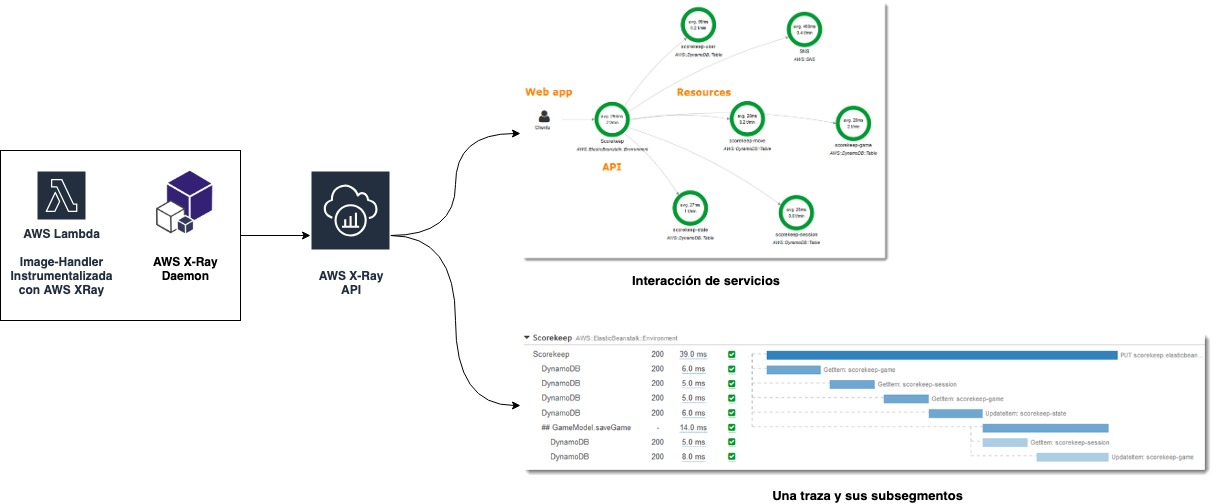
\includegraphics[width=17cm]{image-handler-xray}
  \caption[\emph{Image-Handler} publicando eventos de rendimiento al servicio AWS X-Ray]{\emph{Image-Handler} publicando eventos de rendimiento al servicio AWS X-Ray. Elaboración propia}
  \label{fig:image-handler-xray}
\end{figure}

En la figura \ref{fig:image-handler-xray} se muestran los principales involucrados en la generación de trazas de rendimiento en AWS X-Ray. A la función \emph{Image-Handler} se le agrega la biblioteca de AWS X-Ray para crear las trazas. Estas trazas se envían al servicio AWS X-Ray que recolecta estas trazas, y con base en ellas, se pueden obtener mapas de la interacción de los servicios que componen la función y desgloses de los subsegmentos que componen la traza.


\section{Estrategia de extracción de modelo de rendimiento para \emph{Image-Handler}} \label{sec:estrategia-de-extraccion-de-modelo}
 
Debido a que las funciones Lambda se ejecutan en contenedores que son tanto inaccesibles como efímeros para los diseñadores e implementadores, y sobre los cuales no se tiene ningún control, deben replantearse las estrategias tradicionales en donde se crean bitácoras en la misma computadora donde se ejecuta la aplicación y se van monitoreando utilizando alguna herramienta especializada o simplemente mediante \emph{Secure Socket Channel}(\texttt{SSH}). Para este tipo de software, se hace necesario registrar los eventos asociados al comportamiento del rendimiento en una computadora o servicio externo el cual se tenga control para acceder a los resultados y procesarlos.

Para la extracción del modelo PCM a partir de las bitácoras de Kieker, se llevaron a cabo las siguientes actividades:
\begin{enumerate}
    \item Creación de la versión Image-PK (Sección \ref{sec:image-handler-kieker-pmx}): Versión de \emph{Image-Handler} con las bibliotecas de Kieker para generar bitácoras del rendimiento de la función.    
%    de acuerdo con su manual de usuario\cite{kieker-user-guide}. Se crean objetos de tipo \texttt{OperationExecutionRecord} los cuales contienen información acerca del rendimiento de una invocación sobre alguna parte del código, y luego estos objetos se publican a una cola de mensajería para su posterior tratamiento. En el listado \ref{lst:image-handler-kieker} se puede ver un extracto del código de la función instrumentalizada para que genere objetos  \texttt{OperationExecutionRecord}.
    \item Provisionar una nueva máquina virtual en AWS, en la cual se va a:
    \begin{itemize}
        \item Ejecutar una cola JMS.
        \item Ejecutar una aplicación consumidora de mensajes de la cola JMS.
        \item Almacenar la bitácora de registros de rendimiento de la función Lambda.
    \end{itemize}

    \item Configurar la biblioteca de Kieker para indicar que la publicación de los registros de rendimiento de la función se hagan a través de la cola JMS en la máquina virtual del punto \#2.
    \item Creación de una aplicación consumidora de mensajes para que una vez que arriben los mensajes a la cola JMS, esta procese los mensajes de la cola y los almacene en una bitácora en la máquina virtual creada en el punto \#2. La figura \ref{fig:image-handler-kieker} muestra los involucrados en el proceso de publicación de mediciones de rendimiento del código de \emph{Image-Handler} hacia una bitácora externa.
    \item Una vez obtenida una bitácora en formato Kieker, esta se usó como entrada para PMX. PMX inspecciona la bitácora, la procesa y retorna un archivo \texttt{.zip} con los archivos correspondientes a una instancia de PCM. Lo anterior se aprecia en la figura \ref{fig:image-handler-pmx}.
\end{enumerate}

\newpage
\subsection{Modelo obtenido}
A partir de la bitácora proporcionada como entrada, PMX logró identificar 6 componentes principales:
\begin{itemize} 
    \item \texttt{ImageHandlerKieker}: El punto de entrada de la función.
    \item \texttt{ImageRequestParser}: Encargado de tomar la solicitud de redimensionamiento, analizarla y convertirla en un objeto que pueda ser utilizado por el resto de componentes.
    \item \texttt{S3ImageService}: Contiene la lógica de:
        \begin{enumerate}
            \item Cómo obtener una imagen y
            \item Cómo aplicar la redimensión sobre ella.
        \end{enumerate}
    \item \texttt{S3Dao}: El componente que sabe cómo obtener una imagen el servicio AWS S3
    \item \texttt{AmazonS3Client}: Contiene las operaciones de comunicación de bajo nivel con el servicio AWS.
    \item \texttt{HandlerResponseWriter}: Convierte la imagen redimensionada a una representación en \texttt{Base 64} y prepara la respuesta de la función.
\end{itemize}

Adicionalmente, como parte de las tareas de afinamiento en el modelo, se agregó un nuevo componente al llamado \texttt{AWS Lambda} por medio del cual se representó el efecto que la plataforma AWS Lambda tiene en la invocación a la función. Los detalles acerca de este componente se discuten en mayor detalle en la Sección \ref{sec:experimento-1}. 

Cada uno de los componentes expone su funcionalidad por medio de una interfaz. En el modelado y simulación basado en componentes, los componentes se conciben como piezas intercambiables los cuales exponen sus operaciones por medio de interfaces y delegan los detalles de implementación a componentes concretos (como, por ejemplo, \emph{BasicComponents}). 

Durante las pruebas realizadas al modelo generado por PMX, se percató que si bien el modelo representaba muy bien la intención detrás de los componentes del código fuente, no era detallado en las estimaciones del uso de cada componente. En PCM, a cada componente se le puede especificar su flujo de acciones, estimaciones de rendimiento e invocaciones a otros componentes, por medio de \emph{Service Effect Specifications} (SEFF). 

En principio, las estimaciones incluidas en los SEFFs generados por PMX no lograron ser de utilidad para obtener predicciones representativas de lo observado en las ejecuciones de la función Lambda: mientras que en las invocaciones a \emph{Image-Handler} se entregaban tiempos de respuesta distintos, las simulaciones sobre el modelo entregaban siempre un dato fijo. Las estimaciones de rendimiento de los SEFFs se basaban en tiempos de cómputo constantes, lo que hacía que el motor de simulaciones generara una predicción del tiempo de respuesta con el mismo valor para todos los casos.

En la figura \ref{fig:image-handler-pcm-model} se muestra el modelo de repositorio en \emph{Palladio Component Model} obtenido a partir del proceso de extracción. En este modelo se muestran los tipos de datos, interfaces y componentes de \emph{Image Handler}. Las interfaces contienen la especificación del servicio que proporcionará el componente, mientras que el componente - propiamente- es el que contiene los detalles del cómo llevar a cabo dicha especificación.



%Por esta razón fue se recurrió al trabajo del punto \#3, para obtener datos ``crudos'' del rendimiento de la función Lambda e incluir esto en los \emph{SEFFs} del modelo como distribuciones de frecuencia.



%\begin{lstlisting}[caption={Extracto de la clase \texttt{ImageHandler.java} instrumentalizada con Kieker}, label={lst:image-handler-kieker}]
%public class ImageHandlerKieker implements RequestStreamHandler {
%    private static final IMonitoringController MONITORING_CONTROLLER;
%    static {
%        MONITORING_CONTROLLER = MonitoringController.getInstance();
%    }
%    .
%    .
%    .
%    
%    @Override
%    public void handleRequest(InputStream inputStream, OutputStream outputStream, Context context) throws IOException {
%
%        final long tin = MONITORING_CONTROLLER.getTimeSource().getTime();
%        handleRequestInternal(inputStream, outputStream, context);
%        final long tout = MONITORING_CONTROLLER.getTimeSource().getTime();
%        final OperationExecutionRecord e = new OperationExecutionRecord("public void "+ this.getClass().getName()+".handleRequest(InputStream, OutputStream, Context)",
%                OperationExecutionRecord.NO_SESSION_ID,
%                OperationExecutionRecord.NO_TRACE_ID,
%                tin, tout,
%                InetAddress.getLocalHost().getHostName(),
%                0,
%                0);
%        MONITORING_CONTROLLER.newMonitoringRecord(e);
%    }
%    .
%    .
%    .
%}    
%\end{lstlisting}

% generara registros del rendimiento de la ejecución utilizando las bibliotecas proporcionadas por Kieker, de acuerdo con su manual de usuario\cite{kieker-user-guide}. En lugar de publicar los registros en alguna bitácora local, los registros del rendimiento se publican en una cola \emph{Java Message Service}(JMS). Una vez que arriban los mensajes a la cola JMS, otra aplicación empieza a consumir los mensajes y los va almacenando en una bitácora. 

%La figura \ref{fig:image-handler-kieker} muestra los involucrados en el proceso de publicación de mediciones de rendimiento del código de \emph{Image-Handler} hacia una bitácora externa.

%Una vez que la función Lambda se ejercitó y se haya obtenido una bitácora de Kieker, se toma esta bitácora como entrada para PMX, con el fin de obtener una instancia de PCM. Esto se aprecia en la figura \ref{fig:image-handler-pmx}. Se espera que, al utilizarse datos de mediciones directas del rendimiento de la función Lambda, PMX pueda generar una instacia de PCM que sea confiable y de la que se puedan obtener simulaciones que representativas del comportamiento de la función Lambda.

\begin{figure}[h]
  \centering
  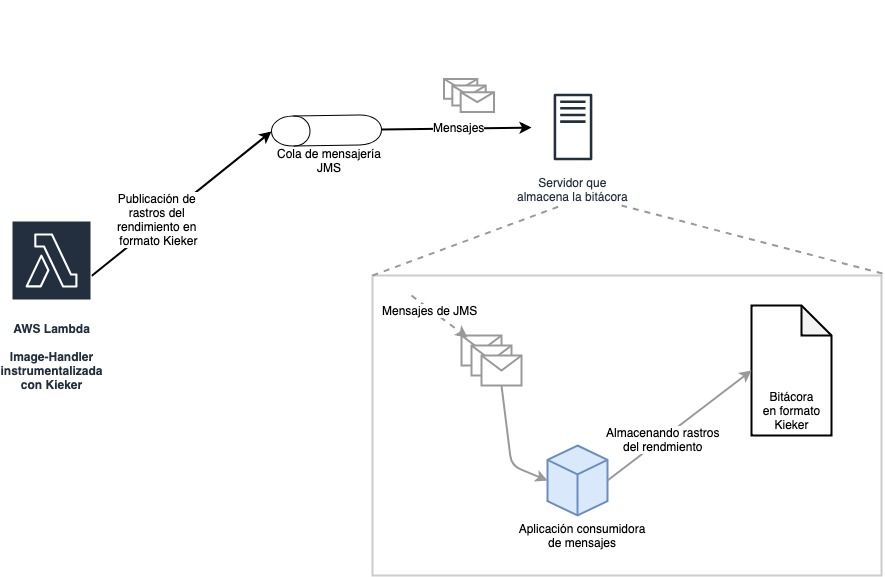
\includegraphics[width=17cm]{image-handler-kieker}
  \caption[Publicación de mediciones del rendimiento de la función Lambda.]{Publicación de mediciones del rendimiento de la función Lambda. Elaboración propia.}
  \label{fig:image-handler-kieker}
\end{figure}

\begin{figure}[h]
  \centering
  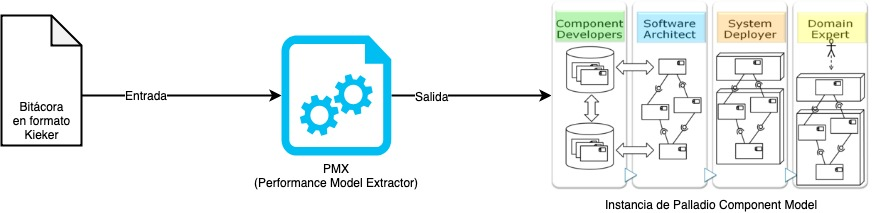
\includegraphics[width=17cm]{image-handler-pmx}
  \caption[Convirtiendo una bitácora de Kieker a una instancia de PCM por medio de PMX.]{Convirtiendo una bitácora de Kieker a una instancia de PCM por medio de PMX. Elaboración propia.}
  \label{fig:image-handler-pmx}
\end{figure}

\subsubsection{Aporte de la versión IM-XRay a las simulaciones}\label{sec:image-handler-xray}
Una actividad recurrente durante el modelado y la simulación de arquitecturas de software, es la del afinamiento del modelo. Esta tarea es necesaria para que el modelo en cual se está trabajando pueda llegar a convertirse una representación cercana del comportamiento de un artefacto de software en escenarios reales. 

Durante el trabajo con el modelo PCM obtenido en la Sección \ref{sec:image-handler-kieker-pmx} se notó que las estimaciones hechas por PMX no correspondían al comportamiento observado y que el esfuerzo necesario para obtener estas estimaciones a partir de las bitácoras de Kieker podría llegar a ser sustancial, principalmente porque el formato de las bitácoras de Kieker incluye muchos más datos que solo las estimaciones de rendimiento y porque se empezó a tener la sensación de que estos datos de alguna u otra forma no estaban ``contando toda la historia'' de lo que estaba pasando con la función Lambda. Por ejemplo, las datos de rendimiento de Kieker no podían explicar tiempos de retraso que se observaban al inicio de la ejecución de la función Lambda y, sin esos datos, se podía llegar a generar un modelo poco preciso.

Por esta razón se comenzó a explorar herramientas alternativas para obtener mediciones del rendimiento de la función Lambda y se eligió Amazon X-Ray para este fin. AWS X-Ray ayuda a los desarrolladores a analizar y depurar aplicaciones distribuidas en producción, tales como las basadas en arquitecturas de microservicios. Con AWS X-Ray se puede ver cómo es que la aplicación y sus servicios asociados se están ejecutando, con miras a identificar y resolver problemas de rendimiento y errores en general.

AWS X-Ray recolecta datos de las solicitudes que hacen a cada uno de los servicios de la aplicación y los agrupa en unas unidades llamadas trazas(\emph{traces}). Luego, utilizando estas trazas, es posible ver mapas de la interacción de los servicios, latencias y metadatos para analizar el comportamiento o identificar problemas.


Las trazas recolectadas en AWS X-Ray fueron de gran utilidad para refinar las estimaciones de rendimiento que cada uno de los componentes identificados realizaba. En el experimento \#1, en la Sección \ref{sec:experimento-1}, se tomaron los datos de rendimiento de cada componente y, se realizaron análisis de frencuencias con el fin de conocer cómo se distribuían los datos con respecto de sus probabilidades. Las probabilidades fueron introducidas en los \emph{SEFFs} de cada componente para la ejecución de simulaciones.   



\eject \pdfpagewidth=28in \pdfpageheight=23in
\begin{landscape}
\thispagestyle{empty}
\begin{figure}[htb]
  \vspace*{3cm} 
  \hspace{-33cm} 
  \centering
  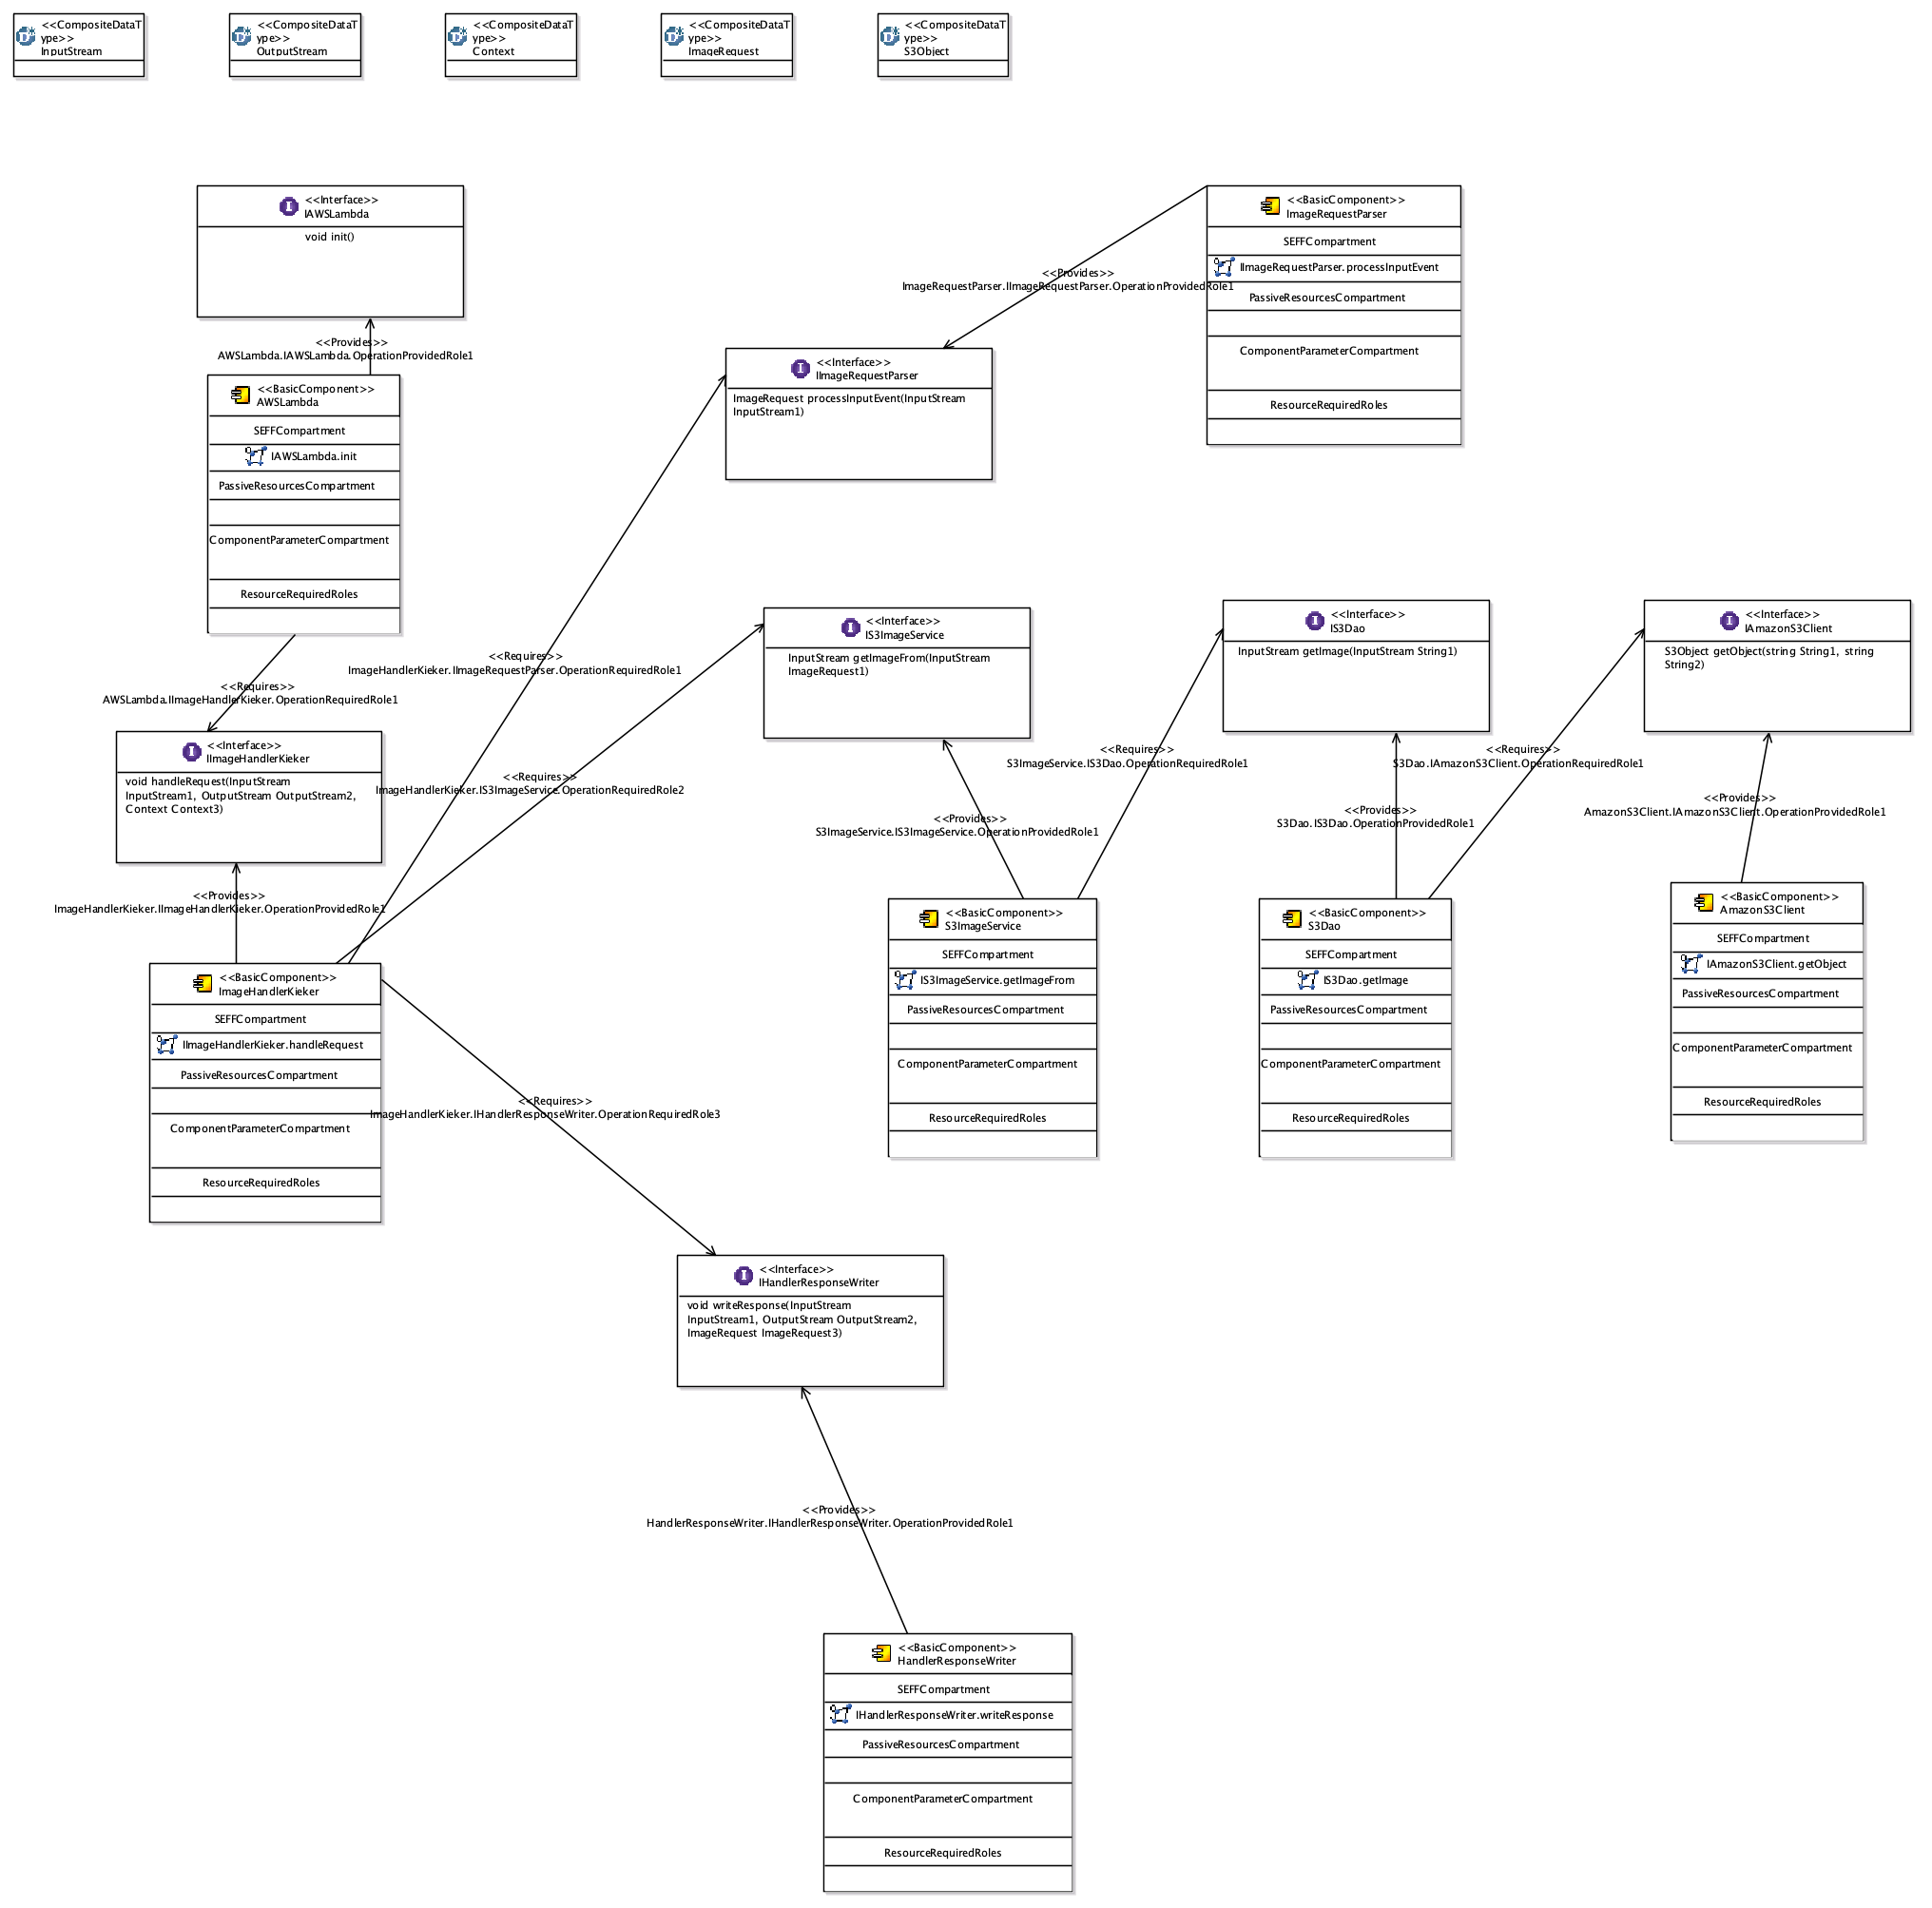
\includegraphics[scale=1.0]{image-handler-extracted-repository-diagram.png}
  \caption[\hspace{0.2cm} Modelo de repositorio en \emph{Palladio Component Model}]{Modelo de repositorio en \emph{Palladio Component Model}: tipos de datos, interfaces y componentes producidos por PMX a partir de una bitácora Kieker. Elaboración propia.}
  \label{fig:image-handler-pcm-model}
\end{figure}
\end{landscape}




\eject \pdfpagewidth=\paperwidth \pdfpageheight=\paperheight



% Rafaga 500Kb en promedio 2min, 45seg
% Rafaga 1Mb en promedio 9 min, 15 seg
% Rafaga 2Mb en promedio 13 min, 15 seg



%\hspace{-3cm}
%\begin{tikzpicture}
%\begin{axis}[
%    width=18cm, height=15cm,
%    title={\textbf{1000 Simulaciones: Función de probabilidad acumulada para los tres escenarios de pruebas }},
%    xlabel={Segundos},
%    ylabel={Probabilidad acumulada},
%    xmin=0, xmax=12,
%    ymin=0, ymax=1.05,
%    extra y ticks = {0.9,0.95},
%    extra x ticks = {1.6, 10.135},
%    extra x tick style={tick label style={font=\footnotesize}},    
%%    legend pos=north east,
%	legend style={at={(0.5,-0.15)},
%		anchor=north,legend columns=-1},
%    grid=major,
%    grid style=dashed,
%]
%
%\addplot[mark=none,blue,smooth] table [col sep=comma] {datos/hasta-500kb-cdf.csv};
%\addplot[mark=none,green,smooth] table [col sep=comma] {datos/hasta-1mb-cdf.csv};
%\addplot[mark=none,orange,smooth] table [col sep=comma] {datos/mas-1mb-cdf.csv};
%
%\coordinate (a) at (axis cs:1.6, 0.95);
%%\draw[blue, dashed, thick](a -| current plot begin) -- (a);
%\draw[blue, dashed, thick](a |- current plot begin) -- (a);
%
%\coordinate (b) at (axis cs:8.0, 0.95);
%%\draw[red, dashed, thick](b -| current plot begin) -- (b);
%\draw[green, dashed, thick](b |- current plot begin) -- (b);
%
%\coordinate (b) at (axis cs:10.135, 0.95);
%%\draw[red, dashed, thick](b -| current plot begin) -- (b);
%\draw[orange, dashed, thick](b |- current plot begin) -- (b);
% 
%\legend{Hasta 500Kb, De 500Kb a 1Mb, Mayor a 1Mb} 
% 
%\end{axis}
%\end{tikzpicture}
%
%
%\hspace{-3.0cm}
%\begin{tikzpicture}
%\begin{axis}[
%  width=19cm, height=8.3cm,
%  title style={align=center},
%  title={Distribución de los tiempos de respuesta en solicitudes de redimensionamiento\\de imágenes de tamaño $\leq 500Kb$ en las simulaciones de Palladio},
%  ylabel={Solicitudes de redimensionamiento},
%  xmin=0, ymin=0, xmax=4000,
%  ybar interval,
%  xtick=data,
%  xticklabel interval boundaries,
%  x tick label style={rotate=45,anchor=east}
%  ],
%	\addplot+[hist={bins=10}]
%		table[col sep=comma, y index=0] {datos/tiempos-de-respuesta-hasta-500kb-palladio.csv};
%\legend{Tiempos de respuesta (En $ms$)}
%\end{axis}
%\end{tikzpicture}
%
%\hspace{-3.0cm}
%\begin{tikzpicture}
%\begin{axis}[
%  width=19cm, height=8.3cm,
%  title style={align=center},
%  title={Distribución de los tiempos de respuesta en solicitudes de redimensionamiento\\de imágenes de tamaño $\leq 500Kb$ en \emph{Image Handler}},
%  ylabel={Solicitudes de redimensionamiento},
%  xmin=0, ymin=0, xmax=4020,
%  ybar interval,
%  xtick=data,
%  xticklabel interval boundaries,
%  x tick label style={rotate=45,anchor=east}
%  ],
%	\addplot+[fill=red!70!white,hist={bins=10}]
%		table[col sep=comma, y index=0] {datos/tiempos-de-respuesta-hasta-500kb-simple.csv};
%\legend{Tiempos de respuesta (En $ms$)}
%\end{axis}
%\end{tikzpicture}
%
%
%% XY PLOT 1
%\hspace{-3cm}
%\begin{tikzpicture}
%	\begin{axis}[
%	width=19cm, height=15cm, xmin=0, ymin=0,
%	xmax=1010, ymax=4500,
%	title={\textbf{1000 Solicitudes de redimensionamiento de imágenes de tamaño $\leq 500Kb$}},
%	xlabel={Número de ejecución de solicitud de redimensionamiento},
%	ylabel={Milisegundos},
%	grid=major, grid style=dashed, label style={font=\small},
%%	extra y ticks={400,600},
%%	extra y tick labels={PP, PIM},
%   extra y tick style={%
%     color=green,
%    },	
%	tick label style={font=\footnotesize},
%	scatter/classes={%
%		a={mark=square*,blue},%
%		b={mark=square*,red},%
%		c={mark=o,draw=black}}]			
%		
%%  \addplot[green,sharp plot,update limits=false] 
%%	coordinates {(0,500) (500,500) (1000,500)} 
%%	node[above] at (axis cs:400,500) {Houses};		
%		
%	\addplot[scatter,only marks,%
%		scatter src=explicit symbolic]%
%	table[meta=label, col sep=comma] {datos/xy-data-hasta-500kb.csv};
%	
%	
%	\legend{Simulaciones de Palladio, Solicitudes a \emph{Image Handler}}
%	\end{axis}
%\end{tikzpicture}

%% --------------------------------------------------

%\hspace{-3.0cm}
%\begin{tikzpicture}
%\begin{axis}[
%  width=19cm, height=8.3cm,
%  title style={align=center},
%  title={Distribución de los tiempos de respuesta en solicitudes de redimensionamiento\\de imágenes de tamaño $500Kb \leq x \leq 1Mb$ en las simulaciones de Palladio},
%  ylabel={Solicitudes de redimensionamiento},
%  xmin=0, ymin=0, xmax=9300,
%  ybar interval,
%  xtick=data,
%  xticklabel interval boundaries,
%  x tick label style={rotate=45,anchor=east}
%  ],
%	\addplot+[hist={bins=10}]
%		table[col sep=comma, y index=0] {datos/tiempos-de-respuesta-hasta-1mb-palladio.csv};
%\legend{Tiempos de respuesta (En $ms$)}
%\end{axis}
%\end{tikzpicture}
%
%\hspace{-3.0cm}
%\begin{tikzpicture}
%\begin{axis}[
%  width=19cm, height=8.3cm,
%  title style={align=center},
%  title={Distribución de los tiempos de respuesta en solicitudes de redimensionamiento\\de imágenes de tamaño $500Kb \leq x \leq 1Mb$ en \emph{Image Handler}},
%  ylabel={Solicitudes de redimensionamiento},
%  xmin=0, ymin=0, xmax=8500,
%  ybar interval,
%  xtick=data,
%  xticklabel interval boundaries,
%  x tick label style={rotate=45,anchor=east}
%  ],
%	\addplot+[fill=red!70!white,hist={bins=10}]
%		table[col sep=comma, y index=0] {datos/tiempos-de-respuesta-hasta-1mb-simple.csv};
%\legend{Tiempos de respuesta (En $ms$)}
%\end{axis}
%\end{tikzpicture}
%
%\hspace{-2cm}
%\begin{tikzpicture}
%	\begin{axis}[
%	width=18cm, height=15cm, xmin=0, ymin=0,
%	xmax=1010, 
%	ymax=9500,
%	title={\textbf{Solicitudes de redimensionamiento de imágenes de tamaño $500Kb \leq x \leq 1Mb$}},
%	xlabel={Número de ejecución de solicitud de redimensionamiento},
%	ylabel={Milisegundos},
%	grid=major, grid style=dashed, label style={font=\small},
%%	extra y ticks={400,600},
%%	extra y tick labels={PP, PIM},
%%   extra y tick style={%
%%     color=green,
%%    },	
%	tick label style={font=\footnotesize},
%	scatter/classes={%
%		a={mark=square*,blue},%
%		b={mark=square*,red},%
%		c={mark=o,draw=black}}]			
%	\addplot[scatter,only marks,%
%		scatter src=explicit symbolic]%
%	table[meta=label, col sep=comma] {datos/xy-data-hasta-1mb.csv};
%	\legend{Simulaciones de Palladio, Solicitudes a \emph{Image Handler}}
%	\end{axis}
%\end{tikzpicture}
%
%\hspace{-3.0cm}
%\begin{tikzpicture}
%\begin{axis}[
%  width=19cm, height=15cm,
%  title={\textbf{Distribución del tamaño de imágenes de tamaño $500Kb \leq x \leq 1Mb$}},
%  ylabel={Cantidad de imágenes},
%  xmin=0, ymin=0, xmin=500, xmax=1024,
%  ybar interval,
%  xtick=data,
%  xticklabel interval boundaries,
%  x tick label style={rotate=45,anchor=east}  
%  ],
%	\addplot+[hist={bins=10}]
%		table[col sep=comma, y index=0] {datos/tamannos-cluster-b.csv};
%\legend{Tamaño de imágenes}
%\end{axis}
%\end{tikzpicture}
%
%%% --------------------------------------------------
%
%\hspace{-3.0cm}
%\begin{tikzpicture}
%\begin{axis}[
%  width=19cm, height=8.3cm,
%  title style={align=center},
%  title={Distribución de los tiempos de respuesta en solicitudes de redimensionamiento\\de imágenes de tamaño $1Mb \leq x \leq 2Mb$ en las simulaciones de Palladio},
%  ylabel={Solicitudes de redimensionamiento},
%  xmin=3700, ymin=0, xmax=14000,
%  ybar interval,
%  xtick=data,
%  xticklabel interval boundaries,
%  x tick label style={rotate=45,anchor=east}
%  ],
%	\addplot+[hist={bins=10}]
%		table[col sep=comma, y index=0] {datos/tiempos-de-respuesta-mas-de-1mb-palladio.csv};
%\legend{Tiempos de respuesta (En $ms$)}
%\end{axis}
%\end{tikzpicture}
%
%\hspace{-2.5cm}
%\begin{tikzpicture}
%\begin{axis}[
%  width=19cm, height=8.3cm,
%  title style={align=center},
%  title={Distribución de los tiempos de respuesta en solicitudes de redimensionamiento\\de imágenes de tamaño $1Mb \leq x \leq 2Mb$ en \emph{Image Handler}},
%  ylabel={Solicitudes de redimensionamiento},
%  xmin=3900, ymin=0, xmax=10000,
%  ybar interval,
%  xtick=data,
%  xticklabel interval boundaries,
%  x tick label style={rotate=45,anchor=east}
%  ],
%	\addplot+[fill=red!70!white,hist={bins=10}]
%		table[col sep=comma, y index=0] {datos/tiempos-de-respuesta-mas-de-1mb-simple.csv};
%\legend{Tiempos de respuesta (En $ms$)}
%\end{axis}
%\end{tikzpicture}
%
%
%% XY Plot 3
%\hspace{-3cm}
%\begin{tikzpicture}
%	\begin{axis}[
%	width=19cm, height=15cm, xmin=0, ymin=0,
%	xmax=1010, 
%	ymax=14500,
%	title={\textbf{Solicitudes de redimensionamiento de imágenes de tamaño $1Mb \leq x \leq 2Mb$}},
%	xlabel={Número de ejecución de solicitud de redimensionamiento},
%	ylabel={Milisegundos},
%	grid=major, grid style=dashed, label style={font=\small},
%	tick label style={font=\footnotesize},
%	scatter/classes={%
%		a={mark=square*,blue},%
%		b={mark=square*,red},%
%		c={mark=o,draw=black}}]			
%	\addplot[scatter,only marks,%
%		scatter src=explicit symbolic]%
%	table[meta=label, col sep=comma] {datos/xy-data-mas-de-1mb.csv};
%	\legend{Simulaciones de Palladio, Solicitudes a \emph{Image Handler}}
%	\end{axis}
%\end{tikzpicture}
%
%\hspace{-3.0cm}
%\begin{tikzpicture}
%\begin{axis}[
%  width=19cm, height=15cm,
%  title={\textbf{Distribución del tamaño de imágenes de tamaño $1Mb \leq x \leq 2Mb$}},
%  ylabel={Cantidad de imágenes},
%  xmin=0, ymin=0, xmin=1000, xmax=2048,
%  ybar interval,
%  xtick=data,
%  xticklabel interval boundaries,
%  x tick label style={rotate=45,anchor=east}  
%  ],
%	\addplot+[hist={bins=10}]
%		table[col sep=comma, y index=0] {datos/tamannos-cluster-c.csv};
%\legend{Tamaño de imágenes}
%\end{axis}
%\end{tikzpicture}
%
%%% --------------------------------------------------
%
%\hspace{-4cm}
%\begin{table}
%    \centering
%    \begin{tabular}{l|r|r|r}
%        \toprule[1.5pt]
%        \multicolumn{4}{c}{\textbf{Hasta 500Kb}} \\
%        \midrule
%        Solicitud de redimensionamiento  & Image Handler & Palladio & Diferencia\\
%        \midrule
%        Tiempo promedio  & 583.842ms & 793.808ms & 209.965ms\\
%        Desviación estándar & 460.659ms & 465.441ms & 4.782ms\\
%        Varianza & 212206.961 & 216635 & -- \\
%        Mediana & 466.715ms & 680.482ms &. -- \\
%        Coeficiente de variación & 0.987 & 0.683 & -- \\
%        \toprule[1.5pt]
%         \multicolumn{4}{c}{\textbf{Entre 500Kb a 1Mb}} \\
%         \midrule 
%        Tiempo promedio  & 4073.600ms & 4348.029ms & 274.428ms\\
%        Desviación estándar & 1731.974ms & 1844.893ms & 112.919ms\\
%        Varianza & 2999736.844 & 3403633.84 & --\\
%        Mediana & 3658.825ms & 3989.406ms & -- \\
%        Coeficiente de variación & 0.473 & 0.462 & -- \\
%        \toprule[1.5pt]
%         \multicolumn{4}{c}{\textbf{Entre 1Mb y 2Mb}} \\
%         \midrule 
%        Tiempo promedio  & 7539.139ms & 7796.913ms & 257.773ms\\
%        Desviación estándar & 1816.152ms & 1914.258ms & 98.106ms \\
%        Varianza & 3298410.017 & 3664385 & -- \\
%        Mediana & 8200.875ms & 8310.293ms & -- \\
%        Coeficiente de variación & 0.221 & 0.230 & -- \\                        
%        \bottomrule[1.5pt]
%    \end{tabular}
%    \caption{Resumen de datos estadísticos}
%\end{table}

\chapter{Diseño Experimental}
\label{cap:diseno-experimental}
En este capítulo se detallan los experimentos realizados para:
\begin{itemize}
    \item Validar si el modelo y la simulaciones sobre este, logran caracterizar el comportamiento de la función \emph{Image Handler} en distintos escenarios, 
    \item Estudiar el comportamiento de la función Lambda cuando es invocada con cargas de trabajo, y
    \item Comparar los resultados de las invocaciones de la función Lambda con los de la herramienta SAM CLI.
\end{itemize}

\section{Utilización \emph{Image-Handler} para redimensionar imágenes de distintos tamaños} \label{sec:experimento-1}
%Este es el caso que se menciona en la Sección \ref{sec:manejador-imagenes-spe} y se muestra en la figura \ref{fig:serverless-image-handler-architecture-workflow}. Se probó la función Lambda con dos imágines: una de tamaño pequeño ($\sim$100Kb) y otra de tamaño grande ($\sim$5Mb). El objetivo es comprobar cómo los distintos tamaños de las imágenes influyen en el tiempo de respuesta de la función.

Este es el caso que se menciona en la Sección \ref{sec:manejador-imagenes-spe} y se muestra en la figura \ref{fig:serverless-image-handler-architecture-workflow}. Se realizaron invocaciones a la función Lambda con tres grupos de imágenes:
\begin{enumerate}
    \item Imágenes de tamaño menor o igual a 500Kb.
    \item Imágenes de tamaño mayor a 500Kb y menor a 1Mb.
    \item Imágenes de tamaño mayor a 1Mb y menor a 2Mb.
\end{enumerate}
Los rangos de tamaños de imágenes se seleccionaron tomando como referencia recomendaciones actuales para el manejo de imágenes para la Web. Las imágenes dentro del primer rango ($x \leq 500Kb$), representan los tamaños de imágenes de uso general sugeridos para contar con sitios Web de buen rendimiento. En los otros dos rangos se agrupan imágenes que tienen el potencial de ser utilizadas en forma más especializada dentro de un sitio Web, por ejemplo aquellas imágenes que suben los usuarios como parte de una red social o imágenes de mayor calidad para enriquecer un diseño, mostrar imágenes asociadas a mapas, entre otros.


En este experimento, el objetivo es comprobar por medio de mediciones directas y de simulaciones en un modelo, cómo los distintos tamaños de las imágenes influyen en el tiempo de respuesta de la función.

Intuitivamente, se espera que, cuando se hagan solicitudes de redimensionamiento de imágenes de mayor tamaño, estas tomen mayor tiempo en ser procesadas y que lo contrario suceda con las imágenes de menor tamaño. Los resultados obtenidos brindan una referencia inicial para saber cómo es que los componentes de software asociados al redimensionamiento trabajan y qué posibles mejoras podrían realizarse.

Las cargas de trabajo para este experimento son de tipo \emph{cerrada}, lo que quiere decir que una solicitud se ejecuta solamente hasta que la anterior se termina (es decir, las invocaciones son estrictamente secuenciales). Esto va orientado a tener mejor trazabilidad de lo que ocurre con la función.


%%%%%%%%%%%%%%%%%%% 1

\subsection{Invocaciones con imágenes menores a 500Kb}
Para la realización de este experimento se contó con la siguiente configuración base:
\begin{itemize}
    \item \emph{Sujeto de prueba:} La función Lambda IM-Simple.
    \item \emph{Repositorio de imágenes:} \emph{Cluster} de 1000 imágenes de tamaño menor a 500Kb alojadas en Amazon S3.     
    \item \emph{Carga de trabajo:} 1000 invocaciones secuenciales de redimensionamiento de imágenes con dimensiones aleatorias a IM-Simple.
    \item \emph{Herramientas de medición:} Amazon Cloudwatch.
\end{itemize}

Configuración para la obtención de datos de rendimiento

\begin{itemize}
    \item \emph{Sujeto de prueba:} Las funciones Lambda IM-KP y IM-XRay
    \item \emph{Repositorio de imágenes:} \emph{Cluster} de 1000 imágenes de tamaño menor a 500Kb alojadas en Amazon S3.     
    \item \emph{Carga de trabajo:} 1000 invocaciones secuenciales de redimensionamiento de imágenes con dimensiones aleatorias a IM-KP y IM-XRay.
    \item \emph{Herramientas de medición:} Kieker, PMX y Amazon X-Ray.
\end{itemize}

Para la realización de este experimento, se obtuvieron 1000 imágenes aleatorias de tamaño menor a 500Kb del servicio \emph{Lorem Picsum}\footnote{\url{https://picsum.photos}}. Se creó un \emph{script} en \texttt{Bash} para acceder a la interfaz de programación (API) proporcionada por \emph{Lorem Picsum} para descargar de forma aleatoria 1000 imágenes cuyo tamaño era menor a los 500Kb. La distribución del tamaño de las 1000 imágenes, en Kb, se aprecia en la figura \ref{fig:distribucion-tamanno-imagenes-hasta-500kb}. El mismo grupo de imágenes se utilizó para realizar solicitudes de redimensionamiento sobre IM-Simple, IM-KP y IM-XRay.

\begin{figure}
\hspace{-1cm}
\begin{tikzpicture}
\begin{axis}[
  width=15cm, height=10cm,
  title={\textbf{Distribución del tamaño de imágenes de tamaño $\leq 500Kb$}},
  ylabel={\small Cantidad de imágenes},
  x label style={at={(axis description cs:0.5,-0.1)},anchor=north},
  xlabel={\small Tamaño de las imágenes (En $Kb$)},
  xmin=0, ymin=0, xmax=550,
  ybar interval,
  xtick=data,
  xticklabel interval boundaries,
  x tick label style={rotate=30,anchor=east}
  ],
	\addplot+[hist={bins=10}]
		table[col sep=comma, y index=0] {datos/tamannos-cluster-a.csv};
\end{axis}
\end{tikzpicture}
\caption[Distribución del tamaño de imágenes $\leq 500Kb$]{Distribución del tamaño de imágenes $\leq 500Kb$. Elaboración propia.}
\label{fig:distribucion-tamanno-imagenes-hasta-500kb}
\end{figure}

\paragraph{Medición Base: 1000 invocaciones de redimensionamiento de imágenes en IM-Simple.} 
Se creó un \emph{script} en \texttt{Bash} para ejecutar 1000 invocaciones de redimensionamiento en la función IM-Simple en las imágenes de tamaño menor a 500Kb. El \emph{script} selecciona una imagen de forma aleatoria y luego ejecuta la solicitud de redimensionamiento utilizando dimensiones de ancho y alto de uso común para imágenes en miniatura (\emph{thumbnails}).

El \emph{script} cuenta con once tamaños para redimensionar las imágenes originales. Estos once tamaños se seleccionaron luego de consultar las guías de referencia en \cite{thumbnail-ref-1, thumbnail-ref-2} sobre tamaños de \emph{thumbnails} en redes sociales tales como Facebook, Twitter, LinkedIn, Pinterest, Tumblr, Instagram y Youtube.

\begin{figure}[h]
\hspace{-1.0cm}
\begin{tikzpicture}
\begin{axis}[
  width=16cm, height=8cm,
  title style={align=center},
  title={\textbf{Distribución de los tiempos de respuesta en solicitudes de redimensionamiento}\\\textbf{de imágenes de tamaño $\leq 500Kb$ en IM-Simple}},
  ylabel={\small Solicitudes de redimensionamiento},
  x label style={at={(axis description cs:0.5,-0.21)},anchor=north},
  xlabel={\small Tiempos de respuesta (En $ms$)},
  xmin=0, ymin=0, xmax=4020,
  ybar interval,
  xtick=data,
  xticklabel interval boundaries,
  x tick label style={rotate=30,anchor=east}
  ],
	\addplot+[fill=red!70!white,hist={bins=10}]
		table[col sep=comma, y index=0] {datos/tiempos-de-respuesta-hasta-500kb-simple.csv};
\end{axis}
\end{tikzpicture}
\caption[Distribución de los tiempos de respuesta en solicitudes de redimensionamiento de imágenes de tamaño $\leq 500Kb$ en IM-Simple]{Distribución de los tiempos de respuesta en solicitudes de redimensionamiento de imágenes de tamaño $\leq 500Kb$ en IM-Simple. Elaboración propia.}
\label{fig:distribucion-solicitudes-imagenes-hasta-500kb}
\end{figure}

\begin{figure}[h]
%\vspace{-4cm}
\hspace{-1.0cm}
\begin{tikzpicture}
\begin{axis}[
  width=16cm, height=8cm,
  title style={align=center},
  title={\textbf{Distribución de los tiempos de respuesta en solicitudes de redimensionamiento}\\\textbf{de imágenes de tamaño $\leq 500Kb$ en las simulaciones de Palladio}},
  ylabel={\small Solicitudes de redimensionamiento},
  xmin=0, ymin=0, xmax=4000,
  ybar interval,
  xtick=data,
  x label style={at={(axis description cs:0.5,-0.2)},anchor=north},
  xlabel={\small Tiempos de respuesta (En $ms$)},  
  xticklabel interval boundaries,
  x tick label style={rotate=30,anchor=east}
  ],
	\addplot+[hist={bins=10}]
		table[col sep=comma, y index=0] {datos/tiempos-de-respuesta-hasta-500kb-palladio.csv};
\end{axis}
\end{tikzpicture}
\caption[Distribución de los tiempos de respuesta en solicitudes de redimensionamiento de imágenes de tamaño $\leq 500Kb$ en las simulaciones de \emph{Palladio Workbench}]{Distribución de los tiempos de respuesta en solicitudes de redimensionamiento de imágenes de tamaño $\leq 500Kb$ en las simulaciones de \emph{Palladio Workbench}. Elaboración propia.}
\label{fig:distribucion-simulacion-imagenes-hasta-500kb}
\end{figure}

En la figura \ref{fig:distribucion-solicitudes-imagenes-hasta-500kb} se muestra la distribución de los tiempos de respuesta en las solicitudes de redimensionamiento en las imágenes de tamaño menor a 500Kb. Con excepción de la primera invocación, la cual tuvo una duración de 4 segundos, más del 97,5\% de las invocaciones no superó los 1,6 segundos.

\paragraph{Mediciones para la obtención de modelo de rendimiento: 1000 invocaciones de redimensionamiento de imágenes en IM-KP y IM-XRay.} Se utilizó el mismo \emph{script} en \texttt{Bash} y la misma configuración para generar invocaciones a la función Lambda descrita en la sección anterior.

En primera instancia se ejecutaron 1000 invocaciones a IM-KP para generar una bitácora de Kieker y a partir de ella extraer un modelo de rendimiento PCM usando PMX. Según se señala en la Sección \ref{sec:image-handler-xray}, las estimaciones hechas por PMX sobre el rendimiento de los componentes del modelo se basaban en valores constantes. Por ello se introdujo IM-XRAY, a fin de contar con una versión alternativa de \emph{Image Handler} que pudiera brindar otro nivel de detalle en las métricas de rendimiento. 

Al igual que en caso anterior, se ejecutaron 1000 invocaciones a IM-XRay, y por medio de un \emph{script} en \texttt{Bash}, se obtuvieron las trazas correspondientes a las 1000 invocaciones. Los nuevos datos fueron exportados a formato \texttt{.csv} e interpretados con el lenguaje \texttt{R}. En \texttt{R}, se calcularon distribuciones de frecuencia de la probabilidad en la que un componente lograba procesar una porción de la carga de trabajo total. Estos datos fueron incluidos en los \emph{SEEFs} de cada componente del modelo. 

Otro valor agregado que brindó IM-XRay a este estudio fue la capacidad de medir el efecto de la plataforma AWS Lambda sobre las invocaciones de redimensionamiento, especialmente durante las primeras invocaciones. Se pudo observar que en las primeras invocaciones de redimensionamiento X-Ray reportaba tiempos de ``inicialización'' y que, cuando esto se daba, la duración total de la invocación de redimensionamiento era mucho mayor al resto. Para incluir estos tiempos de inicialización, se creó un nuevo componente en el modelo con nombre \texttt{AWS Lambda} y, al igual que en los demás componentes, se tomaron los tiempos de inicialización reportados por AWS X-Ray, se exportaron en formato \texttt{.csv} a \texttt{R} para obtener una distribución de frecuencia de la probabilidad e incluirla en los \emph{SEEFs} del componente \texttt{AWS Lambda}. 


Por último se ejecutó una simulación en \emph{Palladio Workbench} con los siguientes parámetros:
\begin{itemize}
    \item Generación de 1000 mediciones.
    \item Carga de trabajo: \emph{cerrada}. Se ejecuta una solicitud sobre el modelo hasta que la anterior termina. 
\end{itemize}

%\hspace{-4cm}
\begin{table}
    \centering
    \begin{tabular}{l|r|r|r}
        \toprule[1.5pt]
        \multicolumn{4}{c}{\textbf{Resumen de datos estadísticos: imágenes $\leq 500Kb$}} \\
        \midrule
        Solicitud de redimensionamiento  & IM-Simple & PCM & Diferencia\\
        \midrule
        Tiempo promedio  & 583.842ms & 793.808ms & 209.965ms\\
        Desviación estándar & 460.659ms & 465.441ms & 4.782ms\\
        Varianza & 212206.961 & 216635.000 & -- \\
        Mediana & 466.715ms & 680.482ms & -- \\
        Coeficiente de variación & 0.987 & 0.683 & -- \\                       
        \bottomrule[1.5pt]
    \end{tabular}
    \caption[Resumen de datos estadísticos: imágenes $\leq 500Kb$]{Resumen de datos estadísticos: imágenes $\leq 500Kb$. Elaboración propia.}
    \label{table:datos-estadisticos-hasta-500kb}
\end{table}

En la figura \ref{fig:distribucion-simulacion-imagenes-hasta-500kb}, se muestra la distribución de los tiempos de respuesta en las solicitudes de redimensionamiento en las simulaciones de \emph{Palladio Workbench} para imágenes de tamaño $\leq 500Kb$. En los resultados de las simulaciones, el 95\% de las invocaciones no superó los 1,6 segundos en procesar la solicitud de redimensionamiento.

En este punto, se cuenta con 1000 mediciones hechas sobre IM-Simple y un modelo al que se le simularon 1000 invocaciones. En la figura \ref{fig:comparacion-imsimple-palladio-500kb} se comparan los tiempos de respuesta obtenidos en IM-Simple y los de las simulaciones, y, en el Cuadro \ref{table:datos-estadisticos-hasta-500kb}, un resumen de los datos estadísticos de los tiempos de respuesta en ambos sujetos de prueba.

\begin{figure}[h]
\hspace{-1cm}
\begin{tikzpicture}
	\begin{axis}[
	width=16cm, height=12cm, xmin=0, ymin=0,
	xmax=1010, ymax=4500,
	title={\textbf{1000 Solicitudes de redimensionamiento de imágenes de tamaño $\leq 500Kb$}},
	xlabel={\small Número de ejecución de solicitud de redimensionamiento},
	ylabel={\small Milisegundos},
	grid=major, grid style=dashed, label style={font=\small},
	legend cell align={left},
%	extra y ticks={400,600},
%	extra y tick labels={PP, PIM},
   extra y tick style={%
     color=green,
    },	
	tick label style={font=\footnotesize},
	scatter/classes={%
		a={mark=square*,blue},%
		b={mark=square*,red},%
		c={mark=o,draw=black}}]					
	\addplot[scatter,only marks,%
		scatter src=explicit symbolic]%
	table[meta=label, col sep=comma] {datos/xy-data-hasta-500kb.csv};
	
	\legend{Simulaciones de Palladio, Solicitudes a IM-Simple}
	\end{axis}
\end{tikzpicture}
\caption[IM-Simple \emph{vs} simulaciones en PCM: 1000 solicitudes de redimensionamiento de imágenes de tamaño $\leq 500Kb$.]{IM-Simple \emph{vs} simulaciones en PCM: 1000 solicitudes de redimensionamiento de imágenes de tamaño $\leq 500Kb$. Elaboración propia.}
\label{fig:comparacion-imsimple-palladio-500kb}
\end{figure}

\begin{figure}[h]
\hspace{-1.5cm}
\begin{tikzpicture}
\begin{axis}[
    width=16cm, height=12cm,
    title={\small \textbf{Probabilidad acumulada: solicitudes de redimensionamiento en imágenes $\leq 500Kb$ en PCM}},
    xlabel={\small Segundos},
    ylabel={\small Probabilidad acumulada},
    xmin=0, xmax=4.2,
    ymin=0, ymax=1.05,
    extra y ticks = {0.9,0.95},
    extra x tick style={tick label style={font=\footnotesize}},    
	legend style={at={(0.5,-0.15)},
		anchor=north,legend columns=-1},
    grid=major,
    grid style=dashed,
]

\addplot[mark=none,blue,smooth,ultra thick] table [col sep=comma] {datos/hasta-500kb-cdf.csv};

\coordinate (a) at (axis cs:1.6, 0.95);
\draw[blue, dashed, ultra thick](a |- current plot begin) -- (a);
 
\end{axis}
\end{tikzpicture}
\caption[Probabilidad acumulada en solicitudes de redimensionamiento en imágenes de tamaño $\leq 500Kb$ en \emph{Palladio Workbench}]{Probabilidad acumulada en solicitudes de redimensionamiento en imágenes de tamaño $\leq 500Kb$ en \emph{Palladio Workbench}. Elaboración propia.}
\label{fig:funcion-acumulada-palladio-500kb}
\end{figure}

\subsection{Análisis de resultados} 
La Figura \ref{fig:comparacion-imsimple-palladio-500kb} muestra un panorama alentador. Las ejecuciones de las simulaciones en PCM presentan tiempos de respuesta muy similares a los que entrega IM-Simple. Hay una diferencia de 209,965ms en el tiempo promedio de los tiempos de respuesta de las simulaciones en PCM con respecto de los tiempos de IM-Simple. Preliminarmente, se valora que, debido a que la versión IM-XRay tiene activado el servicio de monitoreo AWS X-Ray y que fue esta versión de \emph{Image Handler} utilizada como referencia para generar los tiempos procesamiento estimados para cada componente del modelo, instrumentalizar la función Lambda con el servicio de monitoreo AWS X-Ray genera un costo adicional (\emph{overhead}) en el procesamiento de la función. Cabe mencionar que la estrategia de monitoreo utilizada fue muy agresiva, pues para obtener nuevas métricas para los componentes del modelo PCM, se habilitaron muchos puntos de monitoreo dentro del código fuente. Además, se configuró la función Lambda para que monitoreara el 100\% de las invocaciones a solicitudes de redimensionamiento. Esta configuración de monitoreo no es la habitual que se utiliza para las funciones Lambda en producción, pero, para el caso de este estudio se necesitó contar con mayores niveles de detalle en las mediciones, por lo que fue necesario sacar el mayor provecho al monitoreo. Mientras menos sean utilizadas las opciones de monitoreo de AWS X-Ray en la función Lambda, menor será el \emph{overhead} experimentado, como suced con IM-Simple en donde no se experimenta \emph{overhead} por concepto de monitoreo.

Los resultados muestran desviaciones estándar de 460,569ms y 465,445ms para IM-Simple y las simulaciones de PCM respectivamente. La desviación estándar de las simulaciones de PCM es solamente 4,782ms mayor que la de IM-Simple, lo que sugiere que la agrupación de los datos con respecto de su media aritmética serán muy semejantes.

Los coeficientes de variación para IM-Simple y las simulaciones de PCM fue de 0.987 y 0.683 respectivamente. Estos resultados apuntan a una mayor heterogeneidad entre los tiempos de respuesta y a que el tiempo promedio de procesamiento no se considere representativo para este conjunto de datos. Esta variabilidad viene dada por las diferencias de los tamaños de las imágenes utilizadas para este experimento, como se muestra en la Figura \ref{fig:distribucion-tamanno-imagenes-hasta-500kb}: imágenes de tamaño $\leq 500Kb$, en donde existen diferencias de hasta 500x, por lo que, por ejemplo, el tiempo de procesamiento de una imagen de tamaño de 5Kb será significativamente más rápido que una de tamaño de 490Kb.

Por último, de acuerdo con los resultados de las simulaciones, existe un 95\% de probabilidad de que el tiempo de procesamiento de una solicitud de redimensionamiento de una imagen de tamaño $\leq 500Kb$ tome 1,6 segundos o menos (Figura \ref{fig:funcion-acumulada-palladio-500kb}). En IM-Simple, se obtuvo un 97,5\% de probabilidad para el mismo caso (Figura \ref{fig:distribucion-solicitudes-imagenes-hasta-500kb}). Para este caso en particular y, debido a la variabilidad de los tiempos de respuesta, se considera que el uso de esta probabilidad acumulada es más representativa a la hora de describir el comportamiento de la función Lambda.

%%%%%%%%%%%%%%%%%%% 2

\subsection{Invocaciones con imágenes mayores a 500Kb y menores o igual a 1Mb}
Para la realización de este experimento se contó con la siguiente configuración base:
\begin{itemize}
    \item \emph{Sujeto de prueba:} La función Lambda IM-Simple.
    \item \emph{Repositorio de imágenes:} \emph{Cluster} de 1000 imágenes de tamaño mayor a 500Kb y menor o igual a 1Mb alojadas en Amazon S3.     
    \item \emph{Carga de trabajo:} 1000 invocaciones secuenciales de redimensionamiento de imágenes con dimensiones aleatorias a IM-Simple.
    \item \emph{Herramientas de medición:} Amazon Cloudwatch.
\end{itemize}

Configuración para la obtención de datos de rendimiento

\begin{itemize}
    \item \emph{Sujeto de prueba:} La función IM-XRay
    \item \emph{Repositorio de imágenes:} \emph{Cluster} de 1000 imágenes de tamaño mayor a 500Kb y menor o igual a 1Mb alojadas en Amazon S3.     
    \item \emph{Carga de trabajo:} 1000 invocaciones secuenciales de redimensionamiento de imágenes con dimensiones aleatorias a IM-XRay.
    \item \emph{Herramientas de medición:} Amazon X-Ray.
\end{itemize}

Para este experimento no se realizó ningún trabajo sobre la versión IM-KP porque no se necesita extraer ningún modelo. El modelo fue extraído y generado en el experimento anterior y debido a que se usa es el mismo código con los mismos puntos de monitoreo, un eventual proceso de extracción daría como resultado el mismo modelo del experimento anterior. Sí fue necesario calibrar el modelo existente con los resultados de las mediciones a solicitudes de redimensionamiento en imágenes de tamaño mayor a 500Kb y menor o igual 1Mb, utilizando la versión IM-XRay.

Para la realización de este experimento, se obtuvieron 1000 imágenes aleatorias de tamaño mayor a 500Kb y menor o igual a 1Mb del servicio \emph{Lorem Picsum}. Se ejecutó el \emph{script} en \texttt{Bash} del experimento anterior para acceder a la API de \emph{Lorem Picsum} para descargar de forma aleatoria 1000 imágenes cuyo tamaño fuera mayor a los 500Kb y menor o igual a 1Mb. La distribución del tamaño de las 1000 imágenes, en Kb, se aprecia en la figura \ref{fig:distribucion-tamanno-imagenes-hasta-1mb}. El mismo grupo de imágenes se utilizó para realizar solicitudes de redimensionamiento sobre IM-Simple y IM-XRay.

\begin{figure}[h]
\hspace{-1.0cm}
\begin{tikzpicture}
\begin{axis}[
  width=15cm, height=10cm,
  title={\textbf{Distribución del tamaño de imágenes de tamaño $500Kb \leq x \leq 1Mb$}},
  ylabel={\small Cantidad de imágenes},
  x label style={at={(axis description cs:0.5,-0.2)},anchor=north},
  xlabel={\small Tamaño de las imágenes (En $Kb$)},
  xmin=0, ymin=0, xmin=500, xmax=1024,
  ybar interval,
  xtick=data,
  xticklabel interval boundaries,
  x tick label style={rotate=45,anchor=east}  
  ],
	\addplot+[hist={bins=10}]
		table[col sep=comma, y index=0] {datos/tamannos-cluster-b.csv};
\end{axis}
\end{tikzpicture}
\caption[Distribución del tamaño de imágenes $500Kb \leq x \leq 1Mb$]{Distribución del tamaño de imágenes $500Kb \leq x \leq 1Mb$. Elaboración propia.}
\label{fig:distribucion-tamanno-imagenes-hasta-1mb}
\end{figure}

\paragraph{Medición Base: 1000 invocaciones de redimensionamiento de imágenes en IM-Simple.} 
Se ejecutó el \emph{script} en \texttt{Bash} del experimento anterior para ejecutar 1000 invocaciones de redimensionamiento en la función IM-Simple en las imágenes de tamaño mayor a 500Kb y menor o igual a 1Mb. El \emph{script} selecciona una imagen de forma aleatoria y luego ejecuta la solicitud de redimensionamiento utilizando dimensiones de ancho y alto de uso común para imágenes en miniatura.

\begin{figure}[h]
\hspace{-1.0cm}
\begin{tikzpicture}
\begin{axis}[
  width=16cm, height=8cm,
  title style={align=center},
  title={\textbf{Distribución de los tiempos de respuesta en solicitudes de redimensionamiento}\\\textbf{de imágenes de tamaño $500Kb \leq x \leq 1Mb$ en IM-Simple}},
  ylabel={\small Solicitudes de redimensionamiento},
  x label style={at={(axis description cs:0.5,-0.21)},anchor=north},
  xlabel={\small Tiempos de respuesta (En $ms$)},
  xmin=0, ymin=0, xmax=8500,
  ybar interval,
  xtick=data,
  xticklabel interval boundaries,
  x tick label style={rotate=30,anchor=east}
  ],
	\addplot+[fill=red!70!white,hist={bins=10}]
		table[col sep=comma, y index=0] {datos/tiempos-de-respuesta-hasta-1mb-simple.csv};
\end{axis}
\end{tikzpicture}
\caption[Distribución de los tiempos de respuesta en solicitudes de redimensionamiento de imágenes de tamaño $500Kb \leq x \leq 1Mb$ en IM-Simple]{Distribución de los tiempos de respuesta en solicitudes de redimensionamiento de imágenes de tamaño $500Kb \leq x \leq 1Mb$ en IM-Simple. Elaboración propia.}
\label{fig:distribucion-solicitudes-imagenes-hasta-1mb}
\end{figure}


En la figura \ref{fig:distribucion-solicitudes-imagenes-hasta-1mb} se muestra la distribución de los tiempos de respuesta en las solicitudes de redimensionamiento en las imágenes de tamaño mayor a 500Kb y menor o igual a 1Mb. Más del 98\% de las invocaciones no superó los 8 segundos.

\paragraph{Mediciones para la calibración de modelo de rendimiento: 1000 invocaciones de redimensionamiento de imágenes en IM-XRay.} Se utilizó el mismo \emph{script} en \texttt{Bash} y la misma configuración para generar invocaciones a la función Lambda descrita en la sección anterior.

Se ejecutaron 1000 invocaciones a IM-XRay y, por medio de un \emph{script} en \texttt{Bash}, se obtuvieron las trazas correspondientes a las 1000 invocaciones. Los nuevos datos fueron exportados a formato \texttt{.csv} e interpretados con el lenguaje \texttt{R}. En \texttt{R}, se calcularon distribuciones de frecuencia de la probabilidad en la que un componente lograba procesar una porción de la carga de trabajo total. Estos datos fueron incluidos en los \emph{SEEFs} de cada componente del modelo. Por último, se ejecutó una simulación en \emph{Palladio Workbench} con los siguientes parámetros:
\begin{itemize}
    \item Generación de 1000 mediciones.
    \item Carga de trabajo: \emph{cerrada}. Se ejecuta una solicitud sobre el modelo hasta que la anterior termina. 
\end{itemize}

\hspace{-2.0cm}
\begin{figure}
\begin{tikzpicture}
\begin{axis}[
  width=16cm, height=8cm,
  title style={align=center},
  title={\textbf{Distribución de los tiempos de respuesta en solicitudes de redimensionamiento}\\\textbf{de imágenes de tamaño $500Kb \leq x \leq 1Mb$ en las simulaciones de Palladio}},
  ylabel={\small Solicitudes de redimensionamiento},
  x label style={at={(axis description cs:0.5,-0.21)},anchor=north},
  xlabel={\small Tiempos de respuesta (En $ms$)},  
  xmin=0, ymin=0, xmax=9300,
  ybar interval,
  xtick=data,
  xticklabel interval boundaries,
  x tick label style={rotate=30,anchor=east}
  ],
	\addplot+[hist={bins=10}]
		table[col sep=comma, y index=0] {datos/tiempos-de-respuesta-hasta-1mb-palladio.csv};
\end{axis}
\end{tikzpicture}
\caption[Distribución de los tiempos de respuesta en solicitudes de redimensionamiento de imágenes de tamaño $500Kb \leq x \leq 1Mb$ en las simulaciones de Palladio]{Distribución de los tiempos de respuesta en solicitudes de redimensionamiento de imágenes de tamaño $500Kb \leq x \leq 1Mb$ en las simulaciones de Palladio. Elaboración propia.}
\label{fig:distribucion-simulacion-imagenes-hasta-1mb}
\end{figure}

En la figura \ref{fig:distribucion-simulacion-imagenes-hasta-1mb}, se muestra la distribución de los tiempos de respuesta en las solicitudes de redimensionamiento en las simulaciones de \emph{Palladio Workbench} para imágenes de tamaño mayor a 500Kb y menor o igual a 1Mb. En los resultados de las simulaciones, el 95\% de las invocaciones no superó los 8 segundos en procesar la solicitud de redimensionamiento.

En este punto, se cuenta con 1000 mediciones hechas sobre IM-Simple y un modelo al que se le simularon 1000 invocaciones. En la figura \ref{fig:comparacion-imsimple-palladio-1mb} se comparan los tiempos de respuesta obtenidos en IM-Simple y los de las simulaciones, y, en el Cuadro \ref{table:datos-estadisticos-hasta-1mb}, un resumen de los datos estadísticos de los tiempos de respuesta en ambos sujetos de prueba.

\begin{figure}[h]
\hspace{-1cm}
\begin{tikzpicture}
	\begin{axis}[
	width=16cm, height=12cm, xmin=0, ymin=0,
	xmax=1010, 
	ymax=9500,
	legend cell align={left},
	title={\textbf{Solicitudes de redimensionamiento de imágenes de tamaño $500Kb \leq x \leq 1Mb$}},
	xlabel={Número de ejecución de solicitud de redimensionamiento},
	ylabel={Milisegundos},
	grid=major, grid style=dashed, label style={font=\small},
	tick label style={font=\footnotesize},
	scatter/classes={%
		a={mark=square*,blue},%
		b={mark=square*,red},%
		c={mark=o,draw=black}}]			
	\addplot[scatter,only marks,%
		scatter src=explicit symbolic]%
	table[meta=label, col sep=comma] {datos/xy-data-hasta-1mb.csv};
	\legend{Simulaciones de Palladio, Solicitudes a \emph{Image Handler}}
	\end{axis}
\end{tikzpicture}
\caption[Solicitudes de redimensionamiento de imágenes de tamaño $500Kb \leq x \leq 1Mb$]{Solicitudes de redimensionamiento de imágenes de tamaño $500Kb \leq x \leq 1Mb$. Elaboración propia.}
\label{fig:comparacion-imsimple-palladio-1mb}
\end{figure}

\begin{table}
    \centering
    \begin{tabular}{l|r|r|r}
        \toprule[1.5pt]
         \multicolumn{4}{c}{\textbf{Resumen estadístico: imágenes $500Kb \leq x \leq 1Mb$}} \\
        \midrule
        Solicitud de redimensionamiento  & Image Handler & Palladio & Diferencia\\  
        \midrule        
        Tiempo promedio  & 4073.600ms & 4348.029ms & 274.428ms\\
        Desviación estándar & 1731.974ms & 1844.893ms & 112.919ms\\
        Varianza & 2999736.844 & 3403633.840 & --\\
        Mediana & 3658.825ms & 3989.406ms & -- \\
        Coeficiente de variación & 0.473 & 0.462 & -- \\                      
        \bottomrule[1.5pt]
    \end{tabular}
    \caption[Resumen estadístico: imágenes $500Kb \leq x \leq 1Mb$]{Resumen estadístico: imágenes $500Kb \leq x \leq 1Mb$. Elaboración propia.}
    \label{table:datos-estadisticos-hasta-1mb}
\end{table}

\subsection{Análisis de resultados}
A primera vista, la comparación de los tiempos de respuesta de IM-Simple y las simulaciones en PCM mostradas en la Figura \ref{fig:comparacion-imsimple-palladio-1mb} muestran gran similitud. Hay una diferencia de 274,428ms en el tiempo promedio de los tiempos de respuesta en las simulaciones PCM con respecto de los tiempos de IM-Simple. En este experimento también se intuye que la estrategia de monitoreo de AWS X-Ray es la responsable de agregar este \emph{overhead} en el procesamiento.

Los resultados muestran desviaciones estándar de 1731.974ms y 1844.893ms para IM-Simple y las simulaciones de PCM respectivamente. La desviación estándar de las simulaciones de PCM es 112.919ms mayor que la de IM-Simple. Esto indica que la agrupación de los datos con respecto de su media aritmética es muy similar entre ambas muestras.

Los coeficientes de variación de ambas muestras bajaron con respecto a los obtenidos en el primer experimento, aún así, los valores de 0,473 para IM-Simple y de 0,462 para las simulaciones de PCM se consideran heterogéneos, no muy similares entre sí. Esto hace que el tiempo promedio de una solicitud pueda considerarse no tan representativo a la hora de caracterizar el comportamiento de la función Lambda bajo esta carga de trabajo. La variabilidad en los tiempos de respuesta bajó debido a que en los tamaños de las imágenes utilizadas (Figura \ref{fig:distribucion-tamanno-imagenes-hasta-1mb}) tienen una diferencia de hasta 2 veces: es decir, en este conjunto, la imagen más grande es el doble de grande que la imagen más pequeña.

Por último, de acuerdo con los resultados de las simulaciones, existe un 95\% de probabilidad de que el tiempo de procesamiento de una solicitud de redimensionamiento de una imagen de tamaño $500Kb \leq x \leq 1Mb$ tome 8 segundos o menos (Figura \ref{fig:funcion-acumulada-palladio-1mb}). En IM-Simple, se obtuvo un 98\% de probabilidad para el mismo caso (Figura \ref{fig:distribucion-solicitudes-imagenes-hasta-1mb}). Para este caso, como en el experimento anterior, se considera más apropiado el uso de la probabilidad acumulada para describir el comportamiento de la función Lambda.

\begin{figure}[h]
\hspace{-1cm}
\begin{tikzpicture}
\begin{axis}[
    width=16cm, height=12cm,
    title={\small \textbf{Probabilidad acumulada: solicitudes de redimensionamiento en imágenes $500Kb \leq x \leq 1Mb$ en PCM}},
    xlabel={\small Segundos},
    ylabel={\small Probabilidad acumulada},
    xmin=0, xmax=10,
    ymin=0, ymax=1.05,
    extra y ticks = {0.9,0.95},
    extra x tick style={tick label style={font=\footnotesize}},    
	legend style={at={(0.5,-0.15)},
		anchor=north,legend columns=-1},
    grid=major,
    grid style=dashed,
]
\addplot[mark=none,blue,smooth, ultra thick] table [col sep=comma] {datos/hasta-1mb-cdf.csv};
\coordinate (b) at (axis cs:8.0, 0.95);
\draw[blue, dashed, ultra thick](b |- current plot begin) -- (b);
\end{axis}
\end{tikzpicture}
\caption[\hspace{0.2cm} Probabilidad acumulada de solicitudes de redimensionamiento en imágenes $500Kb \leq x \leq 1Mb$ en PCM]{Probabilidad acumulada de solicitudes de redimensionamiento en imágenes $500Kb \leq x \leq 1Mb$ en PCM. Elaboración propia.}
\label{fig:funcion-acumulada-palladio-1mb}
\end{figure}

%%%%%%%%%%%%%%%%%%% 3

\subsection{Invocaciones con imágenes mayores a 1Mb y menores o igual a 2Mb}
Para la realización de este experimento se contó con la siguiente configuración base:
\begin{itemize}
    \item \emph{Sujeto de prueba:} La función Lambda IM-Simple.
    \item \emph{Repositorio de imágenes:} \emph{Cluster} de 1000 imágenes de tamaño mayor a 1Mb y menor o igual a 2Mb alojadas en Amazon S3.     
    \item \emph{Carga de trabajo:} 1000 invocaciones secuenciales de redimensionamiento de imágenes con dimensiones aleatorias a IM-Simple.
    \item \emph{Herramientas de medición:} Amazon Cloudwatch.
\end{itemize}

Configuración para la obtención de datos de rendimiento

\begin{itemize}
    \item \emph{Sujeto de prueba:} La función IM-XRay
    \item \emph{Repositorio de imágenes:} \emph{Cluster} de 1000 imágenes de tamaño mayor a 1Mb y menor o igual a 2mb alojadas en Amazon S3.     
    \item \emph{Carga de trabajo:} 1000 invocaciones secuenciales de redimensionamiento de imágenes con dimensiones aleatorias a IM-XRay.
    \item \emph{Herramientas de medición:} Amazon X-Ray.
\end{itemize}

Al igual que en el experimento de la sección anterior, no se realizó ningún trabajo sobre la versión IM-KP debido a que no era necesario la extracción de un nuevo modelo, sino de, calibrar el modelo existente con los resultados de las mediciones para generar nuevas simulaciones.

Para la realización de este experimento, se obtuvieron 1000 imágenes aleatorias de tamaño mayor a 1Mb y menor o igual a 2Mb del servicio \emph{Lorem Picsum}. Se ejecutó el \emph{script} en \texttt{Bash} del experimento anterior para acceder a la API de \emph{Lorem Picsum} para descargar de forma aleatoria 1000 imágenes cuyo tamaño fuera mayor a 1Mb y menor o igual a 2Mb. La distribución del tamaño de las 1000 imágenes, en Kb, se aprecia en la figura \ref{fig:distribucion-tamanno-imagenes-hasta-2mb}. El mismo grupo de imágenes se utilizó para realizar solicitudes de redimensionamiento sobre IM-Simple y IM-XRay.

\begin{figure}
\hspace{-1.0cm}
\begin{tikzpicture}
\begin{axis}[
  width=15cm, height=10cm,
  title={\textbf{Distribución del tamaño de imágenes de tamaño $1Mb \leq x \leq 2Mb$}},
  ylabel={\small Cantidad de imágenes},
  x label style={at={(axis description cs:0.5,-0.2)},anchor=north},
  xlabel={\small Tamaño de las imágenes (En $Kb$)},  
  xmin=0, ymin=0, xmin=1000, xmax=2048,
  ybar interval,
  xtick=data,
  xticklabel interval boundaries,
  x tick label style={rotate=30,anchor=east}  
  ],
	\addplot+[hist={bins=10}]
		table[col sep=comma, y index=0] {datos/tamannos-cluster-c.csv};
\end{axis}
\end{tikzpicture}
\caption[\hspace{0.2cm} Distribución del tamaño de imágenes de tamaño $1Mb \leq x \leq 2Mb$]{Distribución del tamaño de imágenes de tamaño $1Mb \leq x \leq 2Mb$. Elaboración propia.}
\label{fig:distribucion-tamanno-imagenes-hasta-2mb}
\end{figure}

\paragraph{Medición Base: 1000 invocaciones de redimensionamiento de imágenes en IM-Simple.} 
Se ejecutó el \emph{script} en \texttt{Bash} del experimento anterior para ejecutar 1000 invocaciones de redimensionamiento en la función IM-Simple en las imágenes de tamaño mayor a 1Mb y menor o igual a 2Mb. El \emph{script} selecciona una imagen de forma aleatoria y luego ejecuta la solicitud de redimensionamiento utilizando dimensiones de ancho y alto de uso común para imágenes en miniatura.


\begin{figure}[h]
\hspace{-1.0cm}
\begin{tikzpicture}
\begin{axis}[
  width=16cm, height=8cm,
  title style={align=center},
  title={\textbf{Distribución de los tiempos de respuesta en solicitudes de redimensionamiento}\\\textbf{de imágenes de tamaño $1Mb \leq x \leq 2Mb$ en IM-Simple}},
  ylabel={\small Solicitudes de redimensionamiento},
  x label style={at={(axis description cs:0.5,-0.21)},anchor=north},
  xlabel={\small Tamaño de las imágenes (En $Kb$)},   
  xmin=3900, ymin=0, xmax=10000,
  ybar interval,
  xtick=data,
  xticklabel interval boundaries,
  x tick label style={rotate=45,anchor=east}
  ],
	\addplot+[fill=red!70!white,hist={bins=10}]
		table[col sep=comma, y index=0] {datos/tiempos-de-respuesta-mas-de-1mb-simple.csv};
\end{axis}
\end{tikzpicture}
\caption[\hspace{0.2cm} Distribución de los tiempos de respuesta en solicitudes de redimensionamiento de imágenes de tamaño $1Mb \leq x \leq 2Mb$ en IM-Simple]{Distribución de los tiempos de respuesta en solicitudes de redimensionamiento de imágenes de tamaño $1Mb \leq x \leq 2Mb$ en IM-Simple. Elaboración propia.}
\label{fig:distribucion-solicitudes-imagenes-hasta-2mb}
\end{figure}


En la figura \ref{fig:distribucion-solicitudes-imagenes-hasta-2mb} se muestra la distribución de los tiempos de respuesta en las solicitudes de redimensionamiento en las imágenes de tamaño mayor a 500Kb y menor o igual a 1Mb. Más del 92,5\% de las invocaciones no superó los 9,7 segundos.

\paragraph{Mediciones para la calibración de modelo de rendimiento: 1000 invocaciones de redimensionamiento de imágenes en IM-XRay.} Se utilizó el mismo \emph{script} en \texttt{Bash} y la misma configuración para generar invocaciones a la función Lambda descrita en la sección anterior.

Se ejecutaron 1000 invocaciones a IM-XRay, y por medio de un \emph{script} en \texttt{Bash}, se obtuvieron las trazas correspondientes a las 1000 invocaciones. Los nuevos datos fueron exportados a formato \texttt{.csv} e interpretados con el lenguaje \texttt{R}. En \texttt{R}, se calcularon distribuciones de frecuencia de la probabilidad en la que un componente lograba procesar una porción de la carga de trabajo total. Estos datos fueron incluidos en los \emph{SEEFs} de cada componente del modelo. Por último se ejecutó una simulación en \emph{Palladio Workbench} con los siguientes parámetros:
\begin{itemize}
    \item Generación de 1000 mediciones.
    \item Carga de trabajo: \emph{cerrada}. Se ejecuta una solicitud sobre el modelo hasta que la anterior termina. 
\end{itemize}

\begin{figure}
\hspace{-1cm}
\begin{tikzpicture}
\begin{axis}[
  width=16cm, height=8cm,
  title style={align=center},
  title={\textbf{Distribución de los tiempos de respuesta en solicitudes de redimensionamiento}\\\textbf{de imágenes de tamaño $1Mb \leq x \leq 2Mb$ en las simulaciones de Palladio}},
  ylabel={\small Solicitudes de redimensionamiento},
  x label style={at={(axis description cs:0.5,-0.21)},anchor=north},
  xlabel={\small Tamaño de las imágenes (En $Kb$)}, 
  xmin=3700, ymin=0, xmax=14000,
  ybar interval,
  xtick=data,
  xticklabel interval boundaries,
  x tick label style={rotate=30,anchor=east}
  ],
	\addplot+[hist={bins=10}]
		table[col sep=comma, y index=0] {datos/tiempos-de-respuesta-mas-de-1mb-palladio.csv};
\end{axis}
\end{tikzpicture}
\caption[\hspace{0.2cm} Distribución de los tiempos de respuesta en solicitudes de redimensionamiento de imágenes de tamaño $1Mb \leq x \leq 2Mb$ en las simulaciones de Palladio]{Distribución de los tiempos de respuesta en solicitudes de redimensionamiento de imágenes de tamaño $1Mb \leq x \leq 2Mb$ en las simulaciones de Palladio. Elaboración propia.}
\label{fig:distribucion-simulacion-imagenes-hasta-2mb}
\end{figure}

En la figura \ref{fig:distribucion-simulacion-imagenes-hasta-2mb}, se muestra la distribución de los tiempos de respuesta en las solicitudes de redimensionamiento en las simulaciones de \emph{Palladio Workbench} para imágenes de tamaño mayor a 500Kb y menor o igual a 1Mb. En los resultados de las simulaciones, el 95\% de las invocaciones no superó los 8 segundos en procesar la solicitud de redimensionamiento.

En este punto, se cuenta con 1000 mediciones hechas sobre IM-Simple y un modelo al que se le simularon 1000 invocaciones. En la figura \ref{fig:comparacion-imsimple-palladio-2mb} se comparan los tiempos de respuesta obtenidos en IM-Simple y los de las simulaciones, y, en el Cuadro \ref{table:datos-estadisticos-hasta-2mb}, un resumen de los datos estadísticos de los tiempos de respuesta en ambos sujetos de prueba.

\begin{figure}[h]
\hspace{-1cm}
\begin{tikzpicture}
	\begin{axis}[
	width=16cm, height=12cm, xmin=0, ymin=0,
	xmax=1010, 
	ymax=14500,
	legend cell align={left},
	title={\textbf{Solicitudes de redimensionamiento de imágenes de tamaño $1Mb \leq x \leq 2Mb$}},
	xlabel={\small Número de ejecución de solicitud de redimensionamiento},
	ylabel={\small Milisegundos},
	grid=major, grid style=dashed, label style={font=\small},
	tick label style={font=\footnotesize},
	scatter/classes={%
		a={mark=square*,blue},%
		b={mark=square*,red},%
		c={mark=o,draw=black}}]			
	\addplot[scatter,only marks,%
		scatter src=explicit symbolic]%
	table[meta=label, col sep=comma] {datos/xy-data-mas-de-1mb.csv};
	\legend{Simulaciones de Palladio, Solicitudes a \emph{Image Handler}}
	\end{axis}
\end{tikzpicture}
\caption[\hspace{0.2cm} Solicitudes de redimensionamiento de imágenes de tamaño $1Mb \leq x \leq 2Mb$]{Solicitudes de redimensionamiento de imágenes de tamaño $1Mb \leq x \leq 2Mb$. Elaboración propia.}
\label{fig:comparacion-imsimple-palladio-2mb}
\end{figure}

\begin{table}
    \centering
    \begin{tabular}{l|r|r|r}
        \toprule[1.5pt]
         \multicolumn{4}{c}{\textbf{Resumen de datos estadísticos: imágenes $1Mb \leq x \leq 2Mb$}} \\
         \midrule 
        Tiempo promedio  & 7539.139ms & 7796.913ms & 257.773ms\\
        Desviación estándar & 1816.152ms & 1914.258ms & 98.106ms \\
        Varianza & 3298410.017 & 3664385.000 & -- \\
        Mediana & 8200.875ms & 8310.293ms & -- \\
        Coeficiente de variación & 0.221 & 0.230 & -- \\                        
        \bottomrule[1.5pt]
    \end{tabular}
    \caption[Resumen de datos estadísticos: imágenes $1Mb \leq x \leq 2Mb$]{Resumen de datos estadísticos: imágenes $1Mb \leq x \leq 2Mb$. Elaboración propia.}
    \label{table:datos-estadisticos-hasta-2mb}
\end{table}

\subsection{Análisis de resultados}
Bajo esta carga de trabajo es en donde se puede apreciar mayor similitud en los tiempos de procesamiento de las solicitudes de redimensionamiento entregados por IM-Simple y las simulaciones de PCM. Hay una diferencia de 257,773ms en el tiempo promedio de los tiempos de respuesta en las simulaciones PCM con respecto de los tiempos de IM-Simple. Al igual que en los experimentos anteriores, se considera que la influencia del servicio de monitoreo de AWS X-Ray es el responsable de causar la diferencia en el tiempo de procesamiento.

Los resultados muestran desviaciones estándar de 1816,152ms y 1914.258ms para IM-Simple y las simulaciones de PCM respectivamente. La desviación estándar de las simulaciones de PCM es 98.106ms mayor que la de IM-Simple. Esto indica que el agrupamiento de los datos con respecto de su media aritmética es muy similar entre ambas muestras.

Los coeficientes de variación de son de 0,221 para IM-Simple y de 0,230 para las simulaciones de PCM. Estos resultados son los menores de los tres experimentos y sugieren que los datos son homogéneos entre sí y que, para esta muestra se pueda considerar representativo utilizar el tiempo promedio de respuesta para caracterizar el comportamiento de la función Lambda.

% se consideran heterogéneos, no muy similares entre si. Esto hace que el tiempo promedio de una solicitud pueda considerarse no tan representativo a la hora de caracterizar el comportamiento de la función Lambda bajo esta carga de trabajo. La variabilidad en los tiempos de respuesta bajó debido a que en los tamaños de las imágenes utilizadas (Figura \ref{fig:distribucion-tamanno-imagenes-hasta-1mb}) tienen una diferencia de hasta 2 veces: es decir, en este conjunto, la imagen más grande es el doble de grande que la imagen más pequeña.

Por último, de acuerdo con los resultados de las simulaciones, existe un 95\% de probabilidad de que el tiempo de procesamiento de una solicitud de redimensionamiento de una imagen de tamaño $1Mb \leq x \leq 2Mb$ tome 10,14 segundos o menos (Figura \ref{fig:funcion-acumulada-palladio-2mb}). En IM-Simple, procesar el 100\% de las solicitudes tomó 10 segundos o menos (Figura \ref{fig:distribucion-solicitudes-imagenes-hasta-2mb}). Para este caso, el uso del tiempo promedio de procesamiento de solicitud de redimensionamiento podría ser utilizado para caracterizar el comportamiento de la función Lambda, pero, como en los dos casos anteriores, se considera que el uso de la probabilidad acumulada sea más adecuado para brindar predicciones más acertadas.

%
\begin{figure}
\hspace{-2cm}
\begin{tikzpicture}
\begin{axis}[
    width=16cm, height=12cm,
    title={\hspace{-0.8cm}\textbf{Probabilidad acumulada: solicitudes de redimensionamiento en imágenes $1Mb \leq x \leq 2Mb$ en PCM}},
    xlabel={Segundos},
    ylabel={Probabilidad acumulada},
    xmin=0, xmax=12,
    ymin=0, ymax=1.05,
    extra y ticks = {0.9,0.95},
    extra x tick style={tick label style={font=\footnotesize}},    
	legend style={at={(0.5,-0.15)},
		anchor=north,legend columns=-1},
    grid=major,
    grid style=dashed,
]

\addplot[mark=none,blue,smooth, ultra thick] table [col sep=comma] {datos/mas-1mb-cdf.csv};

\coordinate (b) at (axis cs:10.135, 0.95);
\draw[blue, dashed, ultra thick](b |- current plot begin) -- (b);

\end{axis}
\end{tikzpicture}
\caption[\hspace{0.2cm} Probabilidad acumulada de solicitudes de redimensionamiento en imágenes $1Mb \leq x \leq 2Mb$ en PCM]{Probabilidad acumulada de solicitudes de redimensionamiento en imágenes $1Mb \leq x \leq 2Mb$ en PCM. Elaboración propia.}
\label{fig:funcion-acumulada-palladio-2mb}
\end{figure}

\subsection{Resultados generales}
En los tres experimentos propuestos, los resultados provenientes de las simulaciones lograron caracterizar en gran medida lo observado en IM-Simple. En \ref{fig-probabilidad-acumulada-3-casos} se muestran las 3000 simulaciones realizadas (1000 por cada caso). Las líneas punteadas verticales señalan en dónde se concentran el 95\% de los datos de las simulaciones: 1,6 segundos o menos para las imágnes menores a 500Kb, 8 segundos o menos para las imágenes de entre 500Kb a 1Mb y 10,14 segundos o menos para las imágenes entre 1Mb y 2Mb. 

\begin{figure}
\hspace{-2cm}
\begin{tikzpicture}
\begin{axis}[
    width=16cm, height=12cm,
    title={\textbf{3000 Simulaciones: Función de probabilidad acumulada para los tres escenarios de pruebas}},
    xlabel={\small Segundos},
    ylabel={\small Probabilidad acumulada},
    xmin=0, xmax=12,
    ymin=0, ymax=1.05,
    extra y ticks = {0.9,0.95},
%    extra x ticks = {1.6, 10.135},
    extra x tick style={tick label style={font=\footnotesize}},    
%    legend pos=north east,
	legend style={at={(0.5,-0.15)},
		anchor=north,legend columns=-1},
    grid=major,
    grid style=dashed,
]

\addplot[mark=none,blue,smooth, ultra thick] table [col sep=comma] {datos/hasta-500kb-cdf.csv};
\addplot[mark=none,green,smooth, ultra thick] table [col sep=comma] {datos/hasta-1mb-cdf.csv};
\addplot[mark=none,red,smooth, ultra thick] table [col sep=comma] {datos/mas-1mb-cdf.csv};

\coordinate (a) at (axis cs:1.6, 0.95);
\draw[blue, dashed, thick](a |- current plot begin) -- (a);

\coordinate (b) at (axis cs:8.0, 0.95);
\draw[green, dashed, thick](b |- current plot begin) -- (b);

\coordinate (b) at (axis cs:10.135, 0.95);
\draw[red, dashed, thick](b |- current plot begin) -- (b);
 
\legend{\small Hasta 500Kb, De 500Kb a 1Mb, De 1Mb a 2Mb} 
 
\end{axis}
\end{tikzpicture}
\caption[\hspace{0.2cm} 3000 Simulaciones: Función de probabilidad acumulada para los tres escenarios de pruebas]{3000 Simulaciones: Función de probabilidad acumulada para los tres escenarios de pruebas. Elaboración propia.}
\label{fig-probabilidad-acumulada-3-casos}
\end{figure}

En el Cuadro \ref{table:resumen-estadistico-general} se muestra un resumen estadístico de los tres experimentos llevados a cabo. En este resumen se evidencian los efectos del monitoreo de Amazon X-Ray en la versión IM-XRay de \emph{Image Handler} en el tiempo promedio de procesamiento de una solicitud de redimensionamiento. Las diferencias entre el tiempo promedio de procesamiento en IM-Simple y IM-XRay fue de 209.965ms, 274.428ms y 257.773 para los experimentos \#1, \#2 y \#3, respectivamente. En promedio, hay 247.389ms de diferencia. La desviación estándar de estos tres valores es de 33.463ms y el coeficiente de variación es de 0,13. Estos datos son muy similares entre sí, por ello, para el caso de las simulaciones en PCM es verosímil esperar, en promedio,  diferencias de 247.389ms en los tiempos de respuesta de las simulaciones \emph{versus} los reportados por IM-Simple.

Cabe destacar que las diferencias observadas entre los tiempos de respuesta de las simulaciones con IM-Simple fueron hechas con base en tres valores, los cuales fueron obtenidos a partir de 3000 mediciones bajo tres grupos distintos de imágenes. Por ello los consideramos representativos.

Desde el punto de vista de la arquitectura de software, \emph{Image Handler} muestra mejores rendimientos cuando se prueba con imágenes iguales o menores a 500Kb que con aquellas mayores a ese tamaño. Dentro de las mediciones a los componentes de \emph{Image Handler}, el que experimentó una mayor variabilidad en los tiempos de procesamiento fue el componente de redimensionamiento. Aunque es el componente más importante dentro de esta arquitectura, es también el cuello de botella. Este es el principal componente a ser modificado en aras de probar diferentes comportamientos de \emph{Image Handler}. 

Varias otras optimizaciones podrían ser consideradas aparte de valorar cambios en la biblioteca de redimensionamiento. Aunque puedan existir bibliotecas que logren disminuir el trabajo de redimensionamiento de una imagen, se hace útil también el considerar otras herramientas o estrategias para mejorar los tiempos de respuesta de la función, por ejemplo:
\begin{enumerate}
    \item Limitar el tamaño de las imágenes por procesar: una vez conocido el rendimiento de la función, se podría en limitar las imágenes por procesar con base en sus tamaños por ejemplo, solamente imágenes menores a 500Kb.
    \item Utilizar una memoria intermedia de acceso rápido, un \emph{caché}, para guardar copias de imágenes redimensionadas: después de una primera solicitud de redimensionamiento, se guarda la imagen resultante en un \emph{caché} y luego, entregar esta imagen en subsecuentes solicitudes de redimensionamiento. De esta forma las solicitudes repetitivas no llegarían a ser procesadas por la función Lambda. Esta estrategia se muestra en la Figura \ref{fig:serverless-image-handler-architecture}.
    \item Preprocesar imágenes de gran tamaño fuera de línea: en el caso en donde se cuente con las imágenes originales de antemano, podría ser muy útil ejecutar procesos fuera de línea para redimensionar estas imágenes a los tamaños requeridos y hacer que \emph{Image Handler} solamente sirva estas imágenes y no aplicar ningún tipo de lógica de redimensionamiento.
    \item Como las imágenes son independientes unas de las otras, otra manera de mejorar el rendimiento es vía el lanzamiento concurrente de llamadas a funciones Lambda, bajo el supuesto de que la plataforma aprovisionará varias instancias de la función y, gracias a la separabilidad y no interferencia de los trabajos, se logrará escalabilidad e incremento de eficiencia.  Esto debido a que una vez que se realiza una invocación a una función, esta pasa a un estado activo (caliente - ver Sección \ref{sec:experimento-2-resultados}) y la plataforma ya ha aprovisiado un contenedor que a terminado la ejecución de la función que tenía encargada, por lo que estaría disponible para ejecutar subsecuentes invocaciones de la misma función (con nuevos parámetros de entrada). El cuello de botella podría ser la activación concurrente y la recepción (concurrente) de los resultados, desde la perspectiva del \emph{cliente}.   
    
\end{enumerate}


\hspace{-4cm}
\begin{table}
    \centering
    \begin{tabular}{l|r|r|r}
        \toprule[1.5pt]
        \multicolumn{4}{c}{\textbf{Resumen de datos estadísticos de los tres experimentos propuestos}} \\
        \multicolumn{4}{c}{\textbf{Hasta 500Kb}} \\
        \midrule
        Solicitud de redimensionamiento  & IM-Simple & Palladio & Diferencia\\
        \midrule
        Tiempo promedio  & 583.842ms & 793.808ms & 209.965ms\\
        Desviación estándar & 460.659ms & 465.441ms & 4.782ms\\
        Varianza & 212206.961 & 216635.000 & -- \\
        Mediana & 466.715ms & 680.482ms & -- \\
        Coeficiente de variación & 0.987 & 0.683 & -- \\
        \toprule[1.5pt]
         \multicolumn{4}{c}{\textbf{Entre 500Kb a 1Mb}} \\
         \midrule 
        Tiempo promedio  & 4073.600ms & 4348.029ms & 274.428ms\\
        Desviación estándar & 1731.974ms & 1844.893ms & 112.919ms\\
        Varianza & 2999736.844 & 3403633.840 & --\\
        Mediana & 3658.825ms & 3989.406ms & -- \\
        Coeficiente de variación & 0.473 & 0.462 & -- \\
        \toprule[1.5pt]
         \multicolumn{4}{c}{\textbf{Entre 1Mb y 2Mb}} \\
         \midrule 
        Tiempo promedio  & 7539.139ms & 7796.913ms & 257.773ms\\
        Desviación estándar & 1816.152ms & 1914.258ms & 98.106ms \\
        Varianza & 3298410.017 & 3664385.000 & -- \\
        Mediana & 8200.875ms & 8310.293ms & -- \\
        Coeficiente de variación & 0.221 & 0.230 & -- \\                        
        \bottomrule[1.5pt]
    \end{tabular}
    \caption[Resumen de datos estadísticos de los tres experimentos propuestos]{Resumen de datos estadísticos de los tres experimentos propuestos. Elaboración propia.}
    \label{table:resumen-estadistico-general}
\end{table}




%%%%%%%%%%%%%% Experimento 2
\newpage
\section{Ejecución secuencial ininterrumpida de solicitudes de redimensionamiento}\label{sec:experimento-2}

En el experimento de la Sección \ref{sec:experimento-1} se realizaron múltiples solicitudes de redimensionamiento con el fin de extraer y crear un modelo de rendimiento, ejecutar simulaciones sobre este modelo y comparar los resultados con lo observado en una versión de \emph{Image Handler} real.

Una de las principales inquietudes durante la ejecución de funciones en la nube es determinar si la velocidad en la que se procesa una solicitud resulta ser baja y muestra una tendencia predecible. Los desarrolladores e implementadores necesitan evaluar esto para afinar el código fuente y la arquitectura para evitar cobros elevados por el uso de la plataforma.
De acuerdo con \cite{8360324}, una función puede pasar por dos grandes estados: ``frío'' y ``caliente''. En el estado frío, la plataforma que soporta la función en la nube debe aprovisionar los recursos necesarios para ejecutar la función. Durante esta fase se pueden experimentar los tiempos de respuesta más prolongados. La fase caliente se da luego de que la plataforma que soporta la función reconoce que la función está siendo invocada constantemente y que, debido a este uso, necesita proporcionarle mayores recursos computacionales para brindar mejores tiempos de respuesta. Se espera que, en una función que se esté invocando constantemente, solamente un porcentaje muy bajo del tiempo se encuentre en estado frío y la mayor parte (mientras continúe siendo invocada) estará en estado caliente.

\newpage

\subsection{Ejecución de solicitudes de redimensionamiento simultáneas para imágenes de tamaño menor a 500Kb}

%pic-14.jpeg (500Kb) 8:40 -> 9:05
%pic-27.jpeg (500Kb - 1Mb) 10:45 -> 1am
%pic-175.jpeg (1Mb - 2Mb) 2:16min

Para la realización de este experimento se contó con la siguiente configuración:
\begin{itemize}
    \item \emph{Sujeto de prueba:} La función Lambda IM-Simple.
    \item \emph{Repositorio de imágenes:} \emph{Cluster} de 1000 imágenes de tamaño menor o igual a 500Kb alojadas en Amazon S3.
    \item \emph{Carga de trabajo:} 
    \begin{enumerate}
        \item 1000 invocaciones secuenciales de redimensionamiento de imágenes con dimensiones aleatorias a IM-Simple.
        \item 1000 invocaciones secuenciales de redimensionamiento de una sola imagen a IM-Simple.
    \end{enumerate}
    \item \emph{Herramientas de medición:} Amazon Cloudwatch.
\end{itemize}

En la carga de trabajo \#1, utilizando imágenes aleatorias, la ejecución de las 1000 solicitudes de redimensionamiento fueron las mismas utilizadas para el experimento de la Sección \ref{sec:experimento-1}. 

La ejecución de las 1000 solicitudes de redimensionamiento tomó 2 horas y 36 minutos. Para la carga de trabajo \#2, utilizando una sola imagen, las 1000 solicitudes de redimensionamiento tomaron 25 minutos. Se modificó el \emph{script} en \texttt{Bash} del experimento de la Sección \ref{sec:experimento-1} para elegir aleatoriamente una imagen del \emph{cluster} de 1000 y generar 1000 solicitudes secuenciales a partir de esta con dimensiones de ancho y alto estáticas.

\begin{figure}[h]
\hspace{-1.0cm}
\begin{tikzpicture}
\begin{axis}[
    width=16cm, height=12cm,
    title={\small \textbf{1000 solicitudes de redimensionamiento en imágenes $\leq 500Kb$}},
    xlabel={\small Invocaciones a IM-Simple},
    ylabel={\small Tiempo (en $ms$)},
    xmin=-10, 
    xmax=1005,
    ymin=0, 
%    ymax=4100,
    %extra y ticks = {0.9,0.95},
    extra x tick style={tick label style={font=\footnotesize}},
    grid=major,
    grid style=dashed,
]

\addplot[mark=none,blue,smooth] table [col sep=comma] {datos/tiempos-de-respuesta-hasta-500kb-simple-2.csv};

\addplot[mark=none,red,smooth] table [col sep=comma] {datos/tiempos-de-respuesta-hasta-500kb-simple-una-imagen.csv};

\legend{\small Imágenes aleatorias, \small Imagen única} 
 
\end{axis}
\end{tikzpicture}
% Formato del caption para el índice de figuras %
\caption[\hspace{0.2cm} 1000 solicitudes de redimensionamiento en imágenes $\leq 500Kb$.]{1000 solicitudes de redimensionamiento en imágenes $\leq 500Kb$. La línea azul representa las solicitudes hechas utilizando imágenes aleatorias. La línea roja, las solicitudes utilizando una única imagen. Elaboración propia.}
\label{fig:1000-ejecuciones-secuenciales-500kb}
\end{figure}

En la figura \ref{fig:1000-ejecuciones-secuenciales-500kb} se muestran 1000 ejecuciones secuenciales utilizando imágenes aleatorias (línea azul) y utilizando una sola imagen (línea roja). La imagen de la línea roja es de tamaño 40Kb. Los resultados de los tiempos de respuesta muestran una tendencia marcada: la primera solicitud tomó mucho más tiempo que el resto. Una vez realizada la primera solicitud, los tiempos de respuesta de la función mejoraron considerablemente y no se observaron en las subsecuentes invocaciones tiempos de respuesta que llegaran a ser similares al primero. 


\subsection{Ejecución de solicitudes de redimensionamiento simultáneas para imágenes de tamaño mayor a 500Kb y menor o igual a 1Mb}

Para la realización de este experimento se contó con la siguiente configuración:
\begin{itemize}
    \item \emph{Sujeto de prueba:} La función Lambda IM-Simple.
    \item \emph{Repositorio de imágenes:} \emph{Cluster} de 1000 imágenes de tamaño mayor a 500Kb y menor o igual a 1Mb alojadas en Amazon S3.
    \item \emph{Carga de trabajo:} 
    \begin{enumerate}
        \item 1000 invocaciones secuenciales de redimensionamiento de imágenes con dimensiones aleatorias a IM-Simple.
        \item 1000 invocaciones secuenciales de redimensionamiento de una sola imagen a IM-Simple.
    \end{enumerate}
    \item \emph{Herramientas de medición:} Amazon Cloudwatch.
\end{itemize}

En la carga de trabajo \#1, utilizando imágenes aleatorias, la ejecución de las 1000 solicitudes de redimensionamiento fueron las mismas utilizadas para el experimento de la Sección \ref{sec:experimento-1}. 

La ejecución de las 1000 solicitudes de redimensionamiento tomó 2 horas y 36 minutos. Para la carga de trabajo \#2, utilizando una sola imagen, las 1000 solicitudes de redimensionamiento tomaron 2 horas y 30 minutos. Se modificó el \emph{script} en \texttt{Bash} del experimento de la Sección \ref{sec:experimento-1} para elegir aleatoriamente una imagen del \emph{cluster} de 1000 y generar 1000 solicitudes secuenciales a partir de esta con dimensiones de ancho y alto estáticas.

\begin{figure}[h]
\hspace{-1.5cm}
\begin{tikzpicture}
\begin{axis}[
    width=16cm, height=12cm,
    title={\small \textbf{1000 solicitudes de redimensionamiento en imágenes $500Kb \leq x \leq 1Mb$}},
    xlabel={\small Invocaciones a IM-Simple},
    ylabel={\small Tiempo (en $ms$)},
    xmin=-10, 
    xmax=1005,
    ymin=0, 
    extra x tick style={tick label style={font=\footnotesize}},
    grid=major,
    grid style=dashed,
]

\addplot[mark=none,blue,smooth] table [col sep=comma] {datos/tiempos-de-respuesta-hasta-1mb-simple-2.csv};

\addplot[mark=none,red,smooth] table [col sep=comma] {datos/tiempos-de-respuesta-hasta-1mb-simple-una-imagen.csv};
 
\legend{\small Imágenes aleatorias, \small Imagen única} 

\end{axis}
\end{tikzpicture}
\caption[\hspace{0.2cm} 1000 solicitudes de redimensionamiento en imágenes $500Kb \leq x \leq 1Mb$]{1000 solicitudes de redimensionamiento en imágenes $500Kb \leq x \leq 1Mb$. La línea azul representa las solicitudes hechas utilizando imágenes aleatorias. La línea roja, las solicitudes utilizando una única imagen. Elaboración propia.}
\label{fig:1000-ejecuciones-secuenciales-1mb}
\end{figure}

En la figura \ref{fig:1000-ejecuciones-secuenciales-1mb} se muestran 1000 ejecuciones secuenciales utilizando imágenes aleatorias (línea azul) y utilizando una sola imagen (línea roja). La imagen de la línea roja es de tamaño 750Kb. Los resultados de los tiempos de respuesta muestran una tendencia marcada: la primera solicitud tomó mucho más tiempo que el resto. Una vez realizada la primera solicitud, los tiempos de respuesta de la función mejoraron considerablemente y, en el caso de las solicitudes de redimensionamiento en imágenes aleatorias, sí se logró observar un caso en el que el tiempo de respuesta fue similar al observado en la primera solicitud. En el caso de la imagen única no se observaron tiempos de respuesta que llegaran a ser similares al primero en posteriores invocaciones. 


\subsection{Ejecución de invocaciones de redimensionamiento simultáneas para imágenes de tamaño mayor a 1Mb y menor o igual a 2Mb}

Para la realización de este experimento se contó con la siguiente configuración:
\begin{itemize}
    \item \emph{Sujeto de prueba:} La función Lambda IM-Simple.
    \item \emph{Repositorio de imágenes:} \emph{Cluster} de 1000 imágenes de tamaño mayor a 1Mb y menor o igual a 2Mb alojadas en Amazon S3.
    \item \emph{Carga de trabajo:} 
    \begin{enumerate}
        \item 1000 invocaciones secuenciales de redimensionamiento de imágenes con dimensiones aleatorias a IM-Simple.
        \item 1000 invocaciones secuenciales de redimensionamiento de una sola imagen a IM-Simple.
    \end{enumerate}
    \item \emph{Herramientas de medición:} Amazon Cloudwatch.
\end{itemize}

En la carga de trabajo \#1, utilizando imágenes aleatorias, la ejecución de las 1000 solicitudes de redimensionamiento fueron las mismas utilizadas para el experimento de la Sección \ref{sec:experimento-1}. 

La ejecución de las 1000 solicitudes de redimensionamiento tomó 2 horas y 36 minutos. Para la carga de trabajo \#2, utilizando una sola imagen, las 1000 solicitudes de redimensionamiento tomaron 2 horas y 16 minutos. Se modificó el \emph{script} en \texttt{Bash} del experimento de la Sección \ref{sec:experimento-1} para elegir aleatoriamente una imagen del \emph{cluster} de 1000 y generar 1000 solicitudes secuenciales a partir de esta con dimensiones de ancho y alto estáticas.


\begin{figure}[h]
\hspace{-1.5cm}
\begin{tikzpicture}
\begin{axis}[
    width=16cm, height=12cm,
    title={\small \textbf{1000 solicitudes de redimensionamiento en imágenes $1Mb \leq x \leq 2Mb$}},
    xlabel={\small Invocaciones a IM-Simple},
    ylabel={\small Tiempo (en $ms$)},
    xmin=-10, 
    xmax=1005,
    ymin=0, 
%    ymax=4100,
    %extra y ticks = {0.9,0.95},
    extra x tick style={tick label style={font=\footnotesize}},
    grid=major,
    grid style=dashed,
]

\addplot[mark=none,blue,smooth] table [col sep=comma] {datos/tiempos-de-respuesta-mas-de-1mb-simple-2.csv};

\addplot[mark=none,red,smooth, style={ultra thick}] table [col sep=comma] {datos/tiempos-de-respuesta-mas-de-1mb-simple-una-imagen.csv};

\legend{\small Imágenes aleatorias, \small Imagen única} 
 
\end{axis}
\end{tikzpicture}
\caption[\hspace{0.2cm} 1000 solicitudes de redimensionamiento en imágenes $1Mb \leq x \leq 2Mb$]{1000 solicitudes de redimensionamiento en imágenes $1Mb \leq x \leq 2Mb$. La línea azul representa las solicitudes hechas utilizando imágenes aleatorias. La línea roja, las solicitudes utilizando una única imagen. Elaboración propia.}
\label{fig:1000-ejecuciones-secuenciales-2mb}
\end{figure}

En la figura \ref{fig:1000-ejecuciones-secuenciales-2mb} se muestran 1000 ejecuciones secuenciales utilizando imágenes aleatorias (línea azul) y utilizando una sola imagen (línea roja). La imagen de la línea roja es de tamaño 1,4Mb. Los resultados de los tiempos de respuesta muestran una tendencia similar a los casos anteriores: la primera solicitud tomó mucho más tiempo que el resto. Una vez realizada la primera solicitud, los tiempos de respuesta de la función mejoraron considerablemente y, en el caso de las solicitudes de redimensionamiento en imágenes aleatorias, sí se logró observar un caso en el que el tiempo de respuesta fue similar al observado en la primera solicitud. En el caso de la imagen única no se observaron tiempos de respuesta que llegaran a ser similares al primero en posteriores invocaciones. 

\subsection{Análisis de resultados}\label{sec:experimento-2-resultados}
Luego de las invocaciones de redimensionamiento tanto en imágenes aleatorias como en una sola imagen, se pudo observar que, si bien en las primeras invocaciones se experimentan mayores tiempos de respuesta, los tiempos de respuesta entregados por la función Lambda lograron bajar significativamente y, en los casos de las invocaciones de redimensionamiento en una sola imagen, estos tiempos lograron mantenerse sumamente estables.

Este comportamiento sugiere que en la invocación de una función Lambda en AWS, la plataforma subyacente primero necesita aplicar tareas de aprovisionamiento para poner a disposición la función y, una vez que esto se realiza, la función paulatinamente va pasando a un estado ``caliente'' conforme van arribando las invocaciones de redimensionamiento. Aunque la arquitectura del servicio AWS Lambda no se encuentra disponible públicamente, en artículos en Internet y en proyectos paralelos como \texttt{SAM CLI} y \emph{AWS Lambda container image converter tool}\footnote{\url{https://github.com/awslabs/aws-lambda-container-image-converter}} se sugiere el uso de contenedores Docker que son provisionados con el código de la función y se encargan de procesar las invocaciones entrantes. 

\paragraph{Relación con el modelo de rendimiento obtenido} El modelo de rendimiento obtenido y las simulaciones hechas son agnósticos a los estados ``frío'' o ``caliente'' que se muestran en las observaciones. El principal objetivo de los simuladores de PCM es el de obtener múltiples combinaciones de ejecuciones de una arquitectura de software dada y, a menos que un comportamiento o característica de esta logre ser introducido en el modelo es que su impacto debería reflejarse en las simulaciones.

Si bien en el modelo obtenido no se introdujo esto explícitamente, las mediciones muestran que los tiempos de respuesta más prolongados se corresponden con el momento en que la función estaba en estado ``frío'', por ejemplo, durante las primeras invocaciones. Si se toma como referencia el primer experimento ejecutado en la Sección \ref{sec:experimento-1}, invocaciones de redimensionamiento en imágenes menores o iguales a 500Kb, en la figura \ref{fig:comparacion-imsimple-palladio-500kb}, la primera medición a IM-Simple dio como resultado 4.1s y las subsecuentes 999 invocaciones bajaron a 1.6 segundos o menos; muchas de ellas incluso fueron menores a medio segundo. En los resultados de este experimento, existe un 95\% de probabilidades que los tiempos de respuesta de las invocaciones sean de 1.6 segundos o menos, lo que, visto desde otro ángulo, quiere decir que existe un 5\% de probabilidad que los tiempos de respuesta de las  invocaciones tomen entre 1.6 y 4 segundos en ser procesadas. 

Ahora bien, aunque 5\% parece ser una probabilidad muy alta y que no refleja lo visto en las mediciones, cuando se vuelve a los resultados de las simulaciones se observa que hay probabilidad mayor al 99\% de que una invocación de redimensionamiento tenga un tiempo de respuesta igual o menor a 2 segundos. Esto quiere decir que hay una probabilidad de menos del 1\% de que una invocación a la función Lambda tome entre 2 y 4 segundos en ser procesada. En el caso de las simulaciones de la Figura \ref{fig:comparacion-imsimple-palladio-500kb} solamente 6 casos (de 1000) muestran tiempos de respuesta de entre 2 y 4 segundos lo que representa un 0.006\% del total de las simulaciones realizadas.

Lo anterior señala que, para el caso de \emph{Image Handler}, las simulaciones con los tiempos de respuesta más prolongados representan una cantidad muy pequeña de la totalidad de los casos y que estos casos se pueden interpretar como potenciales escenarios de la función Lambda en estado frío. Las simulaciones muestran que, a pesar del impacto que tienen tales escenarios en las invocaciones, estos realmente no llegan afectar el comportamiento general de la función Lambda. 

Con respecto de los resultados de este experimento y su relación con los escenarios de invocaciones de redimensionamiento en imágenes de tamaño de 500Kb y menor o igual a 1Mb, e imágenes de tamaño de 1Mb y menor a 2Mb, expuestas en la Sección \ref{sec:experimento-1}, se puede emplear un análisis similar: las simulaciones que reportan los tiempos de respuesta más prolongados tienen el potencial de caracterizar las ejecuciones de la función en estado ``frío''.

%%%%%%%%%%%%%% Experimento 3
\section{Variación del intervalo de las invocaciones de redimensionamiento}\label{sec:experimento-3}

Este experimento se plantea como una variante del expuesto en la Sección \ref{sec:experimento-2}, donde se evaluaba el efecto de las invocaciones simultáneas a la función Lambda. Acá se plantea variar el intervalo entre invocaciones a la función Lambda con el fin de valorar los efectos en el comportamiento de la función y si el modelo obtenido en la Sección \ref{sec:experimento-1} contribuye a explicar algo de lo observado; en particular si los intervalos entre las invocaciones hacen que el rendimiento de la función se considere ``fría'' o ``caliente'' en algún punto.

\subsection{Estrategia de intervalo de invocaciones a \emph{Image Handler}}
Para evaluar los efectos de los intervalos de lanzamiento en las invocaciones a \emph{Image Handler}, se propone la ejecución de un número de invocaciones secuencial (una ráfaga), luego entrar en un tiempo de espera y, seguidamente, aplicar otra ráfaga de invocaciones. 

El tiempo de espera entre ráfagas se irá incrementando al doble del tiempo de espera anterior. Por ejemplo, si el primer tiempo de espera es de 2 minutos, el siguiente será de 4 minutos, luego 8, 16, 32 minutos y así sucesivamente. Para este experimento se propone utilizar un tiempo de espera inicial de 10 minutos, para luego aumentarlo en subsecuentes ráfagas de invocaciones.

\subsection{Ejecución de ráfagas de invocaciones de redimensionamiento para imágenes de tamaño menor a 500Kb}

Para la realización de este experimento se utilizó la siguiente configuración base:
\begin{itemize}
    \item \emph{Sujeto de prueba:} La función Lambda IM-XRay.
    \item \emph{Repositorio de imágenes:} \emph{Cluster} de 1000 imágenes de tamaño menor o igual a 500Kb alojadas en Amazon S3.
    \item \emph{Carga de trabajo:} 100 invocaciones secuenciales de redimensionamiento de imágenes con dimensiones aleatorias a IM-XRay seguido de un tiempo de espera de 10, 20 y 40 minutos.      
    \item \emph{Herramientas de medición:} Amazon Cloudwatch y Amazon X-Ray.
\end{itemize}
 
De acuerdo con lo observado en los experimentos anteriores, luego de la primera invocación, las subsiguientes hacen que la función entre en un estado ``caliente''. Por esta razón, ejercitar la función con una ráfaga de 100 invocaciones haría que se logre llegar a este estado fácilmente.

A diferencia de los experimentos anteriores, se utiliza la versión de IM-XRay en lugar de IM-Simple. La razón es que se quiere sacar provecho a las herramientas de monitoreo de AWS X-Ray para determinar si la función pasa de un estado \emph{frío $\rightarrow$ caliente $\rightarrow$ frío} y determinar el impacto de este cambio en el tiempo de respuesta.

\subsection{Variación del intervalo de las invocaciones de redimensionamiento en imágenes $\leq 500Kb$}\label{sec:rafagas-hasta-500kb}

La Figura \ref{fig:rafagas-hasta-500kb} muestra 400 invocaciones de redimensionamiento en imágenes menores a 500Kb divididas en 100 ráfagas cada una. En la primer ráfaga la función se encuentra en estado ``frío'', sucede el aprovisionamiento inicial. Luego de esta primer invocación la función va entrando paulatinamente en estado ``caliente'' y se logra observar que, para la mayoría de los casos las invocaciones de redimensionamiento no llegan a tomar más de 1,5 segundos. El tiempo promedio de ejecución de una ráfaga fue de 2 minutos y 45 segundos.

\begin{figure}[h]
\hspace{-1.0cm}
\begin{tikzpicture}
\begin{axis}[
    width=16cm, height=12cm,
    title={\small \textbf{4 ráfagas de 100 invocaciones de redimensionamiento en imágenes $\leq 500Kb$}},
    xlabel={\small Invocaciones a IM-XRay},
    ylabel={\small Tiempo (en $ms$)},
    xmin=-10, 
    xmax=535,
    ymin=0, 
%    ymax=6000,
%    extra x ticks = {90,165},
    extra x tick style={tick label style={font=\footnotesize}},
    grid=major,
    grid style=dashed,
]

\addplot[mark=none,blue,smooth] table [col sep=comma] {datos/hasta-500kb-rafagas-bck-1.csv};
\addplot[color=red, mark=none, dashed, opacity=0.5, ultra thick] coordinates {(103,0)(103,10000)(117,10000)(117,0)};
\addplot[mark=none,blue,smooth] table [col sep=comma] {datos/hasta-500kb-rafagas-bck-2.csv};
\addplot[color=red, mark=none, dashed, opacity=0.5, ultra thick] coordinates {(223,0)(223,10000)(257,10000)(257,0)};
\addplot[mark=none,blue,smooth] table [col sep=comma] {datos/hasta-500kb-rafagas-bck-3.csv};
\addplot[color=red, mark=none, dashed, opacity=0.5, ultra thick] coordinates {(362,0)(363,10000)(429,10000)(429,0)};
\addplot[mark=none,blue,smooth] table [col sep=comma] {datos/hasta-500kb-rafagas-bck-4.csv};

%\legend{\small Imágenes aleatorias, \small Imagen única} 
 
\end{axis}
\end{tikzpicture}
\caption[\hspace{0.2cm} 4 ráfagas de 100 invocaciones de redimensionamiento en imágenes $\leq 500Kb$]{El espacio delimitado por la línea punteada roja representa 10 minutos de inactividad entre la primera ráfaga y la segunda. El segundo espacio delimitado por la línea punteada roja representa 20 minutos de inactividad entre la segunda y la tercera ráfagas. Elaboración propia}
\label{fig:rafagas-hasta-500kb}
\end{figure}

En la segunda ráfaga, luego de 10 minutos, la función no experimenta un tiempo de respuesta inicial similar al de la primer ráfaga. Esto quiere decir que pasados 10 minutos de inactividad entre la primera y segunda ráfagas, la función continúa en estado caliente.

En la tercera ráfaga, luego de 20 minutos de haberse ejecutado la última invocación de redimensionamiento de la ráfaga anterior, sí se llega observar un tiempo de respuesta inicial alto. AWS X-Ray reporta que en esta invocación inicial se tuvo que re-aprovisionar la función, lo que sugiere que, durante los 20 minutos de inactividad entre una ráfaga y otra, la función fue pasando progresivamente a un estado ``frío'' pues, aparentemente la plataforma pudo determinar que el nivel de actividad de la función (cantidad de invocaciones) fue decreciendo hasta un punto en donde no detectó actividad alguna.

La última ráfaga también experimentó un tiempo de respuesta inicial alto. Esta vez un poco mayor al de la ráfaga anterior pero menor a la de la primera ráfaga. Hubo 40 minutos de inactividad entre la tercera ráfaga y la cuarta. 

\subsection{Variación del intervalo de las invocaciones de redimensionamiento en imágenes $500Kb \leq x \leq 1Mb$}

Se hizo el mismo ejercicio que en la Sección \ref{sec:rafagas-hasta-500kb}, ahora con imágenes entre 500Kb y 1Mb. La Figura \ref{fig:rafagas-hasta-1mb} muestra los resultados de la ejecución de 5 ráfagas de 100 invocaciones cada una. El tiempo promedio de ejecución de una ráfaga fue de 9 minutos y 15 segundos. En la primera invocación de la primera ráfaga se obtuvo un tiempo de respuesta alto (función en estado frío). En la segunda ráfaga no se observó tiempos de respuesta elevados debido a que la función se encontraba en estado ``caliente''. 

\begin{figure}
\hspace{-1cm}
\begin{tikzpicture}
\begin{axis}[
    width=16cm, height=12cm,
    title={\small \textbf{5 ráfagas de 100 invocaciones de redimensionamiento en imágenes $500Kb \leq x \leq 1Mb$}},
    xlabel={\small Invocaciones a IM-XRay},
    ylabel={\small Tiempo (en $ms$)},
    xmin=-10, 
    xmax=775,
    ymin=0, 
    ymax=14000,
%    extra x ticks = {90,165},
    extra x tick style={tick label style={font=\footnotesize}},
    grid=major,
    grid style=dashed,
]

\addplot[mark=none,blue,smooth] table [col sep=comma] {datos/hasta-1mb-rafagas-1.csv};
\addplot[color=red, mark=none, dashed, opacity=0.5, ultra thick] coordinates {(103,0)(103,10000)(117,10000)(117,0)};
\addplot[mark=none,blue,smooth] table [col sep=comma] {datos/hasta-1mb-rafagas-2.csv};
\addplot[color=red, mark=none, dashed, opacity=0.5, ultra thick] coordinates {(223,0)(223,10000)(257,10000)(257,0)};
\addplot[mark=none,blue,smooth] table [col sep=comma] {datos/hasta-1mb-rafagas-3.csv};
\addplot[color=black, mark=none, dashed, style={ultra thick}] coordinates {(260,8082)(260,14000)};
\addplot[color=red, mark=none, dashed, opacity=0.5, ultra thick] coordinates {(362,0)(363,10000)(429,10000)(429,0)};
\addplot[mark=none,blue,smooth] table [col sep=comma] {datos/hasta-1mb-rafagas-4.csv};
\addplot[color=black, mark=none, dashed, style={ultra thick}] coordinates {(434,9356)(434,14000)};
\addplot[color=red, mark=none, dashed, opacity=0.5, ultra thick] coordinates {(535,0)(535,10000)(671,10000)(671,0)};
\addplot[mark=none,blue,smooth] table [col sep=comma] {datos/hasta-1mb-rafagas-5.csv};
 
\end{axis}
\end{tikzpicture}
\caption[\hspace{0.2cm} 5 ráfagas de 100 invocaciones de redimensionamiento en imágenes $500Kb \leq x \leq 1Mb$]{El espacio delimitado por la línea punteada roja representa 10 minutos de inactividad entre la primer ráfaga y la segunda. De ahí en adelante, el espacio delimitado por líneas punteadas rojas corresponde a 20, 40 y 80 minutos de inactividad entre ráfagas. Elaboración propia.}
\label{fig:rafagas-hasta-1mb}
\end{figure}

En la primera invocación de la tercera y cuarta ráfagas, AWS X-Ray reportó que en ambas hubo que re-aprovisionar la función. Es decir, el tiempo de inactividad entre la segunda ráfaga (20 minutos) y entre la tercera y la cuarta (40 minutos) fue suficiente para que la plataforma volviera a marcar la función como fría. Lo interesante de estas dos primeras invocaciones es que aunque la plataforma tuvo que volver a re-aprovisionar la función, los tiempos de respuesta reportados fueron mucho más bajos que el de la invocación inicial de la primera ráfaga. En la Tabla \ref{table:rafagas-hasta-1mb-tiempos-primera-invocacion} se pueden ver los tiempos de respuesta de las primeras invocaciones de cada ráfaga.

\begin{table}
    \centering
    \begin{tabular}{l|r}
        \toprule[1.5pt]
        \multicolumn{2}{c}{\textbf{Entre 500Kb a 1Mb}} \\
        \midrule
        Ráfaga  & Tiempo de 1º invocación \\
        \midrule
        \#1  & 13s \\
        \#2  & N.A. \\        
        \#3  & 8s \\        
        \#4  & 9s \\        
        \#5  & 11s \\                                
        \bottomrule[1.5pt]
    \end{tabular}
    \caption[Tiempo de respuesta de la primera invocación de redimensionamiento en cada ráfaga.]{Tiempo de respuesta de la primera invocación de redimensionamiento en cada ráfaga. Elaboración propia.}
    \label{table:rafagas-hasta-1mb-tiempos-primera-invocacion}
\end{table}

En la quinta ráfaga, el tiempo de respuesta de la primera invocación se elevó de nuevo. El tiempo de inactividad entre la cuarta ráfaga y la quinta fue de 80 minutos. 

Debido a que los tiempos iniciales de la tercera y cuarta ráfaga fueron bajos (aunque AWS X-Ray reporta que para cada uno de ellos fue necesaria re-aprovisionar la función), fue que la ejecución de una quinta ráfaga se hizo necesaria con el fin de validar que, conforme los tiempos de inactividad entre ráfagas aumenta, el tiempo de respuesta de la primera invocación también aumenta. 

\subsection{Variación del intervalo de las invocaciones de redimensionamiento en imágenes $1Mb \leq x \leq 2Mb$}

Para este caso, el tiempo promedio de ejecución de una ráfaga fue de 13 minutos y 15 segundos. En la ejecución de cada ráfaga, AWS X-Ray reportó que fue necesario re-aprovisionar la función cuando se ejecutó la primera invocación de cada ráfaga. En la Figura \ref{fig:rafagas-hasta-2mb} se muestran los resultados de la ejecución de las cuatro ráfagas.

\begin{figure}[h]
\hspace{-1.5cm}
\begin{tikzpicture}
\begin{axis}[
    width=16cm, height=12cm,
    title={\small \textbf{4 ráfagas de 100 invocaciones de redimensionamiento en imágenes $1Mb \leq x \leq 2Mb$}},
    xlabel={\small Invocaciones a IM-XRay},
    ylabel={\small Tiempo (en $ms$)},
    xmin=-10, 
    xmax=535,
    ymin=0, 
    ymax=16000,
%    extra x ticks = {90,165},
    extra x tick style={tick label style={font=\footnotesize}},
    grid=major,
    grid style=dashed,
]

\addplot[mark=none,blue,smooth] table [col sep=comma] {datos/hasta-2mb-rafagas-1.csv};
\addplot[color=red, mark=none, dashed, opacity=0.5, ultra thick] coordinates {(103,0)(103,10000)(117,10000)(117,0)};
\addplot[mark=none,blue,smooth] table [col sep=comma] {datos/hasta-2mb-rafagas-2.csv};
\addplot[color=red, mark=none, dashed, opacity=0.5, ultra thick] coordinates {(223,0)(223,10000)(257,10000)(257,0)};
\addplot[mark=none,blue,smooth] table [col sep=comma] {datos/hasta-2mb-rafagas-3.csv};
\addplot[color=red, mark=none, dashed, opacity=0.5, ultra thick] coordinates {(362,0)(363,10000)(429,10000)(429,0)};
\addplot[mark=none,blue,smooth] table [col sep=comma] {datos/hasta-2mb-rafagas-4.csv};
 
\end{axis}
\end{tikzpicture}
\caption[\hspace{0.2cm} 4 ráfagas de 100 invocaciones de redimensionamiento en imágenes $1Mb \leq x \leq 2Mb$]{El espacio delimitado por la línea punteada roja representa 10 minutos de inactividad entre la primera ráfaga y la segunda. Luego de esto, el espacio delimitado por líneas punteadas rojas corresponde a 20, 40 y 80 minutos de inactividad entre ráfagas. Elaboración propia.}
\label{fig:rafagas-hasta-2mb}
\end{figure}

Los tiempos de respuesta de las primeras invocaciones de cada ráfaga resultaron ser más similares entre sí y también se pudo observar que cuando existen tiempos de inactividad más prolongados, como el que hay entre la ráfaga tres y la cuatro que es de 40 minutos, a la siguiente invocación le toma un mayor tiempo de respuesta que la primera invocación de la ráfaga anterior.

\subsection{Análisis de resultados}
La principal observación que arrojó este experimento es que conforme van aumentando los tiempos de inactividad en la función Lambda, también van aumentando los tiempos de respuesta entregados por la primera invocación luego de este tiempo de inactividad. 

De acuerdo con \cite{cold-starts-aws-lambda-1}, una vez que una función ha sido instalada en la plataforma, la primera invocación debe pasar por el proceso de aprovisionamiento. Después de procesar la primera invocación, la función pasa a un estado activo o ``caliente'' y el contenedor que la soporta se puede reutilizar para subsecuentes invocaciones. Cuando se detecta que la función se vuelve inactiva o ``fría'', el contenedor que la soporta se vuelve candidato a ser ``reciclado'' para que pueda ser utilizado por otra función que lo necesite.

Si bien no es posible conocer con certeza la existencia de un tiempo límite definido para decidir cuándo el contenedor va a ser reciclado o no, los resultados de este experimento y los expuestos en \cite{cold-starts-aws-lambda-1} y \cite{cold-starts-aws-lambda-2} demuestran que entre mayores sean los tiempos de inactividad de una función, mayor será la probabilidad de que el contenedor que la soporta sea reciclado y que, cuando se vuelva a invocar a la función, se experimente un tiempo de respuesta mayor al promedio debido al proceso de aprovisionamiento. 

Según las mediciones en \cite{cold-starts-aws-lambda-1}, el tiempo de vida de un contenedor no parece darse en forma determinística pero se estima que está entre los 25 a 65 minutos. Un contenedor inactivo casi siempre se mantiene vivo por 25 minutos, luego de eso la probabilidad de que sea desechado crece lentamente y llega a alcanzar el 100\% luego de alrededor de 1 hora posterior a la última invocación.

\paragraph{Relación con el modelo de rendimiento obtenido} En el experimento de la Sección \ref{sec:experimento-1} se obtuvo un modelo de rendimiento a partir de una sola ráfaga de invocaciones secuenciales de redimensionamiento. No se introdujeron tiempos de inactividad. 

Aquí, aunque se introducen tiempos de inactividad entre ráfagas, se presenta una tendencia que se ha repetido a lo largo de los tres experimentos ejecutados hasta este momento: las primeras invocaciones reportan mayores tiempos de respuesta, especialmente la primera invocación y, conforme la función va recibiendo más y más invocaciones, su tiempo de respuesta tiende a bajar considerablemente. Esta es una característica que el modelo obtenido logró reconocer y, de igual manera que en los experimentos anteriores, las invocaciones en donde los tiempos de respuesta fueron mayores representan un porcentaje muy bajo ($\approx$ 1\%) del total de invocaciones en una ráfaga. Cuando el modelo reporte invocaciones con tiempos de respuesta alto se puede afirmar, para el caso de \emph{Image Handler}, que estas serán muy pocas y que probablemente representen momentos en donde la función tuvo que pasar forzosamente de un estado ``frío'' a uno ``caliente''.


En PCM, el comportamiento asociado a las invocaciones basadas en ráfagas y tiempos de inactividad podría llegar a ser introducido con un modelo de uso personalizado el cual pueda tomar en cuenta las particularidades del cómo es que una arquitectura de software puede ser potencialmente utilizada, pero la forma en la que PCM reporta los resultados de las simulaciones es la misma - independientemente del modelo de uso (o de cualquier otro modelo) utilizado. Es por esto que, en términos de resultados, PCM siempre va a entregarlos con base en la probabilidad de que una determinada simulación se ejecute en una arquitectura dada. Se indica lo anterior para aclarar que mientras se utilice PCM para ejecutar simulaciones mediante el esquema de ráfaga/tiempo de espera, los resultados obtenidos no vendrán dados de forma específica para cada ráfaga ejecutada, sino más bien serán presentados de forma general.

%%%%%%%%%%%%%% Experimento 4
\section{Comparación de \texttt{SAM CLI} con observaciones reales de AWS Lambda}\label{sec:experimento-4} 
\emph{Serverless Application Model} o \texttt{SAM CLI} es la primera herramienta desarrollada por Amazon para probar funciones Lambda localmente, es decir, sin necesidad de probarlas en la plataforma AWS (en la nube de Amazon). \texttt{SAM CLI} permite desarrollar funciones Lambda en cualquiera de los lenguajes de programación soportados por el servicio AWS Lambda y probarlos sin necesidad de instalarlos directamente en el servicio. A fin de emular el servicio, \texttt{SAM CLI} hace uso de Docker para instalar y ejecutar el código de una función en un contenedor especializado para tal fin. 

\texttt{SAM CLI} no es la primera herramienta desarrollada para probar, instalar y emular funciones Lambda en un entorno local, pero sí es la primera desarrollada por Amazon por lo que se espera que mediante su uso se pueda tener una aproximación muy cercana del comportamiento que tendrá una función Lambda cuando esté en producción.

En este experimento se propone explorar el comportamiento de \emph{Image Handler} cuando se ejecutan invocaciones de redimensionamiento en \texttt{SAM CLI} y comparar lo obtenido con invocaciones de redimensionamiento efectuadas en el servicio de AWS Lambda en producción. Los resultados de este experimento permitirán determinar si las invocaciones hechas en \texttt{SAM CLI} entregan tiempos de respuesta similares a los del servicio AWS Lambda para que, de esta forma, se pueda considerar \texttt{SAM CLI} como una herramienta confiable para simulación de invocaciones de rendimiento.

La versión de \texttt{SAM CLI} utilizada para la realización de todos los experimentos descritos a continuación es \texttt{0.10.0}.

\subsection{Estrategia de comparación de invocaciones de redimensionamiento en \texttt{SAM CLI} y AWS Lambda}

Similar a los experimentos anteriores, se propone ejecutar 1000 ejecuciones de redimensionamiento a \emph{Image Handler}. Para valorar la similitud entre los resultados, el conjuntos\ de invocaciones utilizadas serán las mismas para \texttt{SAM CLI} y AWS Lambda: la $k-$ésima invocación a \emph{Image Handler} realizada por medio de \texttt{SAM CLI} será igual a la $k-$ésima invocación realizada en AWS Lambda.

\subsection{Ejecución de 1000 invocaciones de redimensionamiento para imágenes de tamaño menor a 500Kb}

Para la realización de este experimento se utilizó la siguiente configuración base:
\begin{itemize}
    \item \emph{Sujeto de prueba:} La función lambda IM-Simple.
    \item \emph{Repositorio de imágenes:} \emph{Cluster} de 1000 imágenes de tamaño menor o igual a 500Kb.
    \item \emph{Carga de trabajo:} 1000 invocaciones secuenciales de redimensionamiento de imágenes en IM-Simple.
    \item \emph{Herramientas de medición:} Amazon Cloudwatch.
\end{itemize}

Configuración para la realización del experimento en \texttt{SAM CLI}:
\begin{itemize}
    \item \emph{Sujeto de prueba:} La función lambda IM-Simple.
    \item \emph{Ambiente:} \texttt{SAM CLI} instalado en máquina virtual alojada en el servicio AWS EC2\footnote{\url{https://aws.amazon.com/ec2/}}, de tipo \texttt{t2.large}\footnote{\url{https://aws.amazon.com/ec2/instance-types/t2/}}.
    \item \emph{Repositorio de imágenes:} \emph{Cluster} de 1000 imágenes de tamaño menor o igual a 500Kb.
    \item \emph{Carga de trabajo:} 1000 invocaciones secuenciales de redimensionamiento de imágenes en IM-Simple.
    \item \emph{Herramientas de medición:} Bitácoras de \texttt{SAM CLI}.
\end{itemize}


\begin{figure}[h]
\hspace{-1cm}
\begin{tikzpicture}
	\begin{axis}[
	width=16cm, height=12cm, xmin=0, ymin=0,
	xmax=1010, 
%	ymax=14500,
	title={\textbf{\emph{Image Handler vs} \texttt{SAM CLI}: redimensionamiento en imágenes de tamaño $\leq 500Kb$}},
	xlabel={\small Número de ejecución de solicitud de redimensionamiento},
	ylabel={\small Milisegundos},
	grid=major, grid style=dashed, label style={font=\small},
	tick label style={font=\footnotesize},
	legend cell align={left},
	scatter/classes={%
		a={mark=square*,blue},%
		b={mark=square*,red},%
		c={mark=o,draw=black}}]			
	\addplot[scatter,only marks,%
		scatter src=explicit symbolic]%
	table[meta=label, col sep=comma] {datos/xy-sam-data-500kb.csv};
	\legend{Solicitudes a \emph{Image Handler}, Solicitudes en \texttt{SAM CLI}}
	\end{axis}
\end{tikzpicture}
\caption[\hspace{0.2cm} Solicitudes de redimensionamiento de imágenes de tamaño $1Mb \leq x \leq 2Mb$]{Solicitudes de redimensionamiento de imágenes de tamaño $1Mb \leq x \leq 2Mb$. Elaboración propia.}
\label{fig:comparacion-sam-500kb}
\end{figure}

\begin{table}
    \centering
    \begin{tabular}{l|r|r|r}
        \toprule[1.5pt]
         \multicolumn{4}{c}{\textbf{AWS Lambda vs SAM CLI: imágenes $x \leq 500Kb$}} \\
         \midrule
         & AWS Lambda & \texttt{SAM CLI} & Diferencia \\ 
         \midrule
        Duración & 15min & 90min & -- \\
        Tiempo promedio  & 571.15ms & 804.35ms & 233.20ms\\
        Desviación estándar & 449.76ms & 162.22ms & 287.54ms \\
        Varianza & 202281.41 & 26314.94 & -- \\
        Mediana & 698.28ms & 771.52ms & -- \\
        Coeficiente de variación & 0.64 & 0.21 & -- \\                        
        \bottomrule[1.5pt]
    \end{tabular}
    \caption[AWS Lambda vs SAM CLI: imágenes $x \leq 500Kb$]{Resumen de datos estadísticos. Elaboración propia}
    \label{table:sam-datos-estadisticos-hasta-500kb}
\end{table}

\paragraph{Resultados:} La Figura \ref{fig:comparacion-sam-500kb}, muestra la comparación de los tiempos de respuesta de las 1000 invocaciones realizadas y en la tabla \ref{table:sam-datos-estadisticos-hasta-500kb} un resumen de los datos estadísticos obtenidos. A primera vista se puede ver que el conjunto de tiempos de respuesta de las invocaciones cuando se utilizó \texttt{SAM CLI} fue más homogéneo que las invocaciones en AWS Lambda. Esto también se refleja en los coeficientes de variación: 0.64 y 0.21 para las invocaciones en AWS Lambda y \texttt{SAM CLI} respectivamente, lo que claramente sugiere que el conjunto de tiempos de respuesta obtenido de las invocaciones de \texttt{SAM CLI} es más homogéneo que el de AWS Lambda. Esto también lo confirma una menor desviación estándar en el conjunto de tiempos de respuesta de las invocaciones hechas mediantes \texttt{SAM CLI}. 

En la tabla \ref{table:sam-datos-estadisticos-hasta-500kb}, el tiempo promedio de las invocaciones realizadas en AWS Lambda fue más bajo que el de \texttt{SAM CLI}. En \texttt{SAM CLI}, el menor tiempo de respuesta fue de 545.74ms mientras que en los resultados obtenidos de AWS Lambda aproximadamente el 56\% de los resultados estuvo por debajo de los 545.74ms. Esto indica que, a pesar que el conjunto de los tiempos de respuesta de \texttt{SAM CLI} es más homogéneo, los tiempos obtenidos de AWS Lambda muestran un mejor rendimiento.

\subsection{Ejecución de 1000 invocaciones de redimensionamiento para imágenes de tamaño $500Kb \leq x \leq 1Mb$}

Para la realización de este experimento se utilizó la siguiente configuración base:
\begin{itemize}
    \item \emph{Sujeto de prueba:} La función lambda IM-Simple.
    \item \emph{Repositorio de imágenes:} \emph{Cluster} de 1000 imágenes de tamaño mayor a 500Kb y menor o igual a 1Mb.
    \item \emph{Carga de trabajo:} 1000 invocaciones secuenciales de redimensionamiento de imágenes en IM-Simple.
    \item \emph{Herramientas de medición:} Amazon Cloudwatch.
\end{itemize}

Configuración para la realización del experimento en \texttt{SAM CLI}:
\begin{itemize}
    \item \emph{Sujeto de prueba:} La función lambda IM-Simple.
    \item \emph{Ambiente:} \texttt{SAM CLI} instalado en máquina virtual alojada en el servicio AWS EC2, de tipo \texttt{t2.large}.
    \item \emph{Repositorio de imágenes:} \emph{Cluster} de 1000 imágenes de tamaño mayor o igual a 500Kb y menor a 1Mb.
    \item \emph{Carga de trabajo:} 1000 invocaciones secuenciales de redimensionamiento de imágenes en IM-Simple.
    \item \emph{Herramientas de medición:} Bitácoras de \texttt{SAM CLI}.
\end{itemize}

\begin{figure}
\hspace{-1cm}
\begin{tikzpicture}
	\begin{axis}[
	width=16cm, height=12cm, xmin=0, ymin=0,
	xmax=1010, 
%	ymax=14500,
	title={\textbf{\emph{Image Handler vs} \texttt{SAM CLI}: redimensionamiento en imágenes de tamaño $500Kb \leq x \leq 1Mb$}},
	xlabel={\small Número de ejecución de solicitud de redimensionamiento},
	ylabel={\small Milisegundos},
	grid=major, grid style=dashed, label style={font=\small},
	legend cell align={left},
	tick label style={font=\footnotesize},
	scatter/classes={%
		a={mark=square*,blue},%
		b={mark=square*,red},%
		c={mark=o,draw=black}}]			
	\addplot[scatter,only marks,%
		scatter src=explicit symbolic]%
	table[meta=label, col sep=comma] {datos/xy-sam-data-1mb.csv};
	\legend{Solicitudes a \emph{Image Handler}, Solicitudes en \texttt{SAM CLI}}
	\end{axis}
\end{tikzpicture}
\caption[\hspace{0.2cm} Solicitudes de redimensionamiento de imágenes de tamaño $500kb \leq x \leq 1Mb$]{Solicitudes de redimensionamiento de imágenes de tamaño $500kb \leq x \leq 1Mb$. Elaboración propia.}
\label{fig:comparacion-sam-1mb}
\end{figure}

\begin{table}[h]
    \centering
    \begin{tabular}{l|r|r|r}
        \toprule[1.5pt]
         \multicolumn{4}{c}{\textbf{AWS Lambda vs SAM CLI: imágenes $500Kb \leq x \leq 1Mb$}} \\
         \midrule
         & AWS Lambda & \texttt{SAM CLI} & Diferencia \\ 
         \midrule
        Duración & 72min & 218min & -- \\
        Tiempo promedio  & 4345.80ms & 1969.49ms & 2376.31ms\\
        Desviación estándar & 1867.64ms & 524.95ms & 1342.69ms \\
        Varianza & 3488063.00 & 275569.63 & -- \\
        Mediana & 3898.82ms & 1851.99ms & -- \\
        Coeficiente de variación & 0.48 & 0.28 & -- \\                        
        \bottomrule[1.5pt]
    \end{tabular}
    \caption[AWS Lambda vs SAM CLI: imágenes $500Kb \leq x \leq 1Mb$]{Resumen de datos estadísticos. Elaboración propia.}
    \label{table:sam-datos-estadisticos-hasta-1mb}
\end{table}

\paragraph{Resultados:} El 99.8\% del conjunto de los tiempos de respuesta en \texttt{SAM CLI} se agruparon entre los 1.1 y 3.1 segundos mientras que el 66.8\% del conjunto de los tiempos de respuesta en AWS Lambda estuvieron por encima de los 3.1 segundos. Los tiempos de respuesta de las mediciones hechas en \texttt{SAM CLI} se siguen mostrando mucho más homogéneos que los de AWS Lambda pero, al igual que en el experimento anterior, esto no es una indicación de similitud entre los dos conjuntos de datos. 

En general, los resultados obtenidos de \texttt{SAM CLI} muestran mejor rendimiento que los de AWS Lambda pero no logran caracterizar lo visto en las observaciones en el ambiente de producción. Los tiempos promedios de 4345.80ms y 1969.49ms en AWS Lambda y \texttt{SAM CLI}, respectivamente, aunados con los valores de las desviaciones estándar de 1867.64ms y 524ms para el mismo caso, sugieren que estos conjuntos de datos tienen comportamientos diferentes entre sí.

Por último, a \texttt{SAM CLI} le tomó 218 minutos en procesar las 1000 invocaciones de redimensionamiento, mientras que a AWS Lambda le tomó 72 minutos. Individualmente, las invocaciones de redimensionamiento de \texttt{SAM CLI} muestran mejores tiempos, pero el proceso en general toma más tiempo. A \texttt{SAM CLI} le toma más tiempo aprovisionar sus recursos antes de cada invocación, pero en la bitácora solamente se reporta el tiempo de procesamiento de la invocación como tal. En las condiciones actuales no es posible observar el tiempo de aprovisionamiento en \texttt{SAM CLI}.


\subsection{Ejecución de 1000 invocaciones de redimensionamiento para imágenes de tamaño $1Mb \leq x \leq 2Mb$}

Para la realización de este experimento se utilizó la siguiente configuración base:
\begin{itemize}
    \item \emph{Sujeto de prueba:} La función lambda IM-Simple.
    \item \emph{Repositorio de imágenes:} \emph{Cluster} de 1000 imágenes de tamaño mayor a 1Mb y menor o igual a 2Mb.
    \item \emph{Carga de trabajo:} 1000 invocaciones secuenciales de redimensionamiento de imágenes en IM-Simple.
    \item \emph{Herramientas de medición:} Amazon Cloudwatch.
\end{itemize}

Configuración para la realización del experimento en \texttt{SAM CLI}:
\begin{itemize}
    \item \emph{Sujeto de prueba:} La función lambda IM-Simple.
    \item \emph{Ambiente:} \texttt{SAM CLI} instalado en máquina virtual alojada en el servicio AWS EC2, de tipo \texttt{t2.large}.
    \item \emph{Repositorio de imágenes:} \emph{Cluster} de 1000 imágenes de tamaño mayor o igual a 1Mb y menor a 2Mb.
    \item \emph{Carga de trabajo:} 1000 invocaciones secuenciales de redimensionamiento de imágenes en IM-Simple.
    \item \emph{Herramientas de medición:} Bitácoras de \texttt{SAM CLI}.
\end{itemize}

\begin{figure}[h]
\hspace{-1cm}
\begin{tikzpicture}
	\begin{axis}[
	width=16cm, height=12cm, xmin=0, ymin=0,
	xmax=1010, 
%	ymax=14500,
	title={\textbf{\emph{Image Handler vs} \texttt{SAM CLI}: redimensionamiento en imágenes de tamaño $1Mb \leq x \leq 2Mb$}},
	xlabel={\small Número de ejecución de solicitud de redimensionamiento},
	ylabel={\small Milisegundos},
	grid=major, grid style=dashed, label style={font=\small},
	legend cell align={left},
	tick label style={font=\footnotesize},
	scatter/classes={%
		a={mark=square*,blue},%
		b={mark=square*,red},%
		c={mark=o,draw=black}}]			
	\addplot[scatter,only marks,%
		scatter src=explicit symbolic]%
	table[meta=label, col sep=comma] {datos/xy-sam-data-2mb.csv};
	\legend{Solicitudes a \emph{Image Handler}, Solicitudes en \texttt{SAM CLI}}
	\end{axis}
\end{tikzpicture}
\caption[\hspace{0.2cm} Solicitudes de redimensionamiento de imágenes de tamaño $1Mb \leq x \leq 2Mb$]{Solicitudes de redimensionamiento de imágenes de tamaño $1Mb \leq x \leq 2Mb$. Elaboración propia.}
\label{fig:comparacion-sam-2mb}
\end{figure}

\begin{table}[h]
    \centering
    \begin{tabular}{l|r|r|r}
        \toprule[1.5pt]
         \multicolumn{4}{c}{\textbf{AWS Lambda vs SAM CLI: imágenes $1Mb \leq x \leq 2Mb$}} \\
         \midrule
         & AWS Lambda & \texttt{SAM CLI} & Diferencia \\ 
         \midrule
        Duración & 120min & 225min & -- \\
        Tiempo promedio  & 7113.377ms & 2840.91ms & 4272.464ms\\
        Desviación estándar & 1768.520ms & 494ms & 1268.523ms \\
        Varianza & 3106479.237 & 244032.830 & -- \\
        Mediana & 7785.15ms & 3053.72ms & -- \\
        Coeficiente de variación & 0.226 & 0.16 & -- \\                        
        \bottomrule[1.5pt]
    \end{tabular}
    \caption[AWS Lambda vs SAM CLI: imágenes $1Mb \leq x \leq 2Mb$]{Resumen de datos estadísticos. Elaboración propia.}
    \label{table:sam-datos-estadisticos-hasta-2mb}
\end{table}

\paragraph{Resultados} En este experimento, los dos conjuntos obtenidos resultaron ser los más disímiles entre sí. Solamente el 0,2\% de las invocaciones realizadas por medio de \texttt{SAM CLI} se encontraron en el dentro del rango de tiempo de las invocaciones directas en AWS Lambda. Los datos de la tabla \ref{table:sam-datos-estadisticos-hasta-2mb} confirman que estos dos conjuntos de datos se comportan de manera muy diferente. 

La duración total de todas las invocaciones de redimensionamiento fue de 120 minutos cuando se utilizó la función Lambda de forma directa y de 225 minutos con \texttt{SAM CLI}, similar a los tiempos del experimento anterior. Los tiempos de respuesta obtenidos cuando se usó \texttt{SAM CLI} fueron mejores que las invocaciones directas pero estas no pueden ser utilizadas como una referencia para predecir el comportamiento de la función Lambda cuando se redimensionen imágenes de tamaño a 1Mb y menor o igual 2Mb.

\subsection{\texttt{SAM CLI} como herramienta para la simulación en \emph{Image Handler}}
Los resultados de los experimentos realizados no sugieren que el uso de \texttt{SAM CLI} sea adecuado como herramienta para tener algún grado de predicción del cómo se van a comportar las invocaciones de redimensionamiento a \emph{Image Handler} cuando estén ejecutándose en AWS Lambda.

El escenario que presentó mayor similitud fue con las invocaciones de redimensionamiento en imágenes menores a los 500Kb. En este caso, al menos el 100\% de las invocaciones realizadas por medio de \texttt{SAM CLI} se ubicaron dentro del rango de los tiempos de respuesta cuando se usó AWS Lambda. Conforme se fue incrementando el tamaño de las imágenes a redimensionar, las diferencias en los tiempos de respuesta de un conjunto con respecto del otro se hicieron más notables. Esto hace que para el caso de \emph{Image Handler}, \texttt{SAM CLI} no se considere confiable para caracterizar el comportamiento de la función en un ambiente en producción. Pese a esto, no se pone en duda la utilidad de \texttt{SAM CLI} para la implementación, pruebas e instalación de funciones Lambda en AWS.

%% Para glosario y acronimos
%Some \gls{unadeca}, \acrlong{gcd} \acrshort{gcd}


%\subsection{Resumen de resultados de los cuatros principales experimentos propuestos}
%\paragraph{Experimento \#1} El primer experimento de la Sección \ref{sec:experimento-1} estuvo dirigido a generar un modelo de rendimiento a partir de las bitácoras de la función \emph{Image Handler}. Para esto, se implementó una versión de la función que estuvo instrumentalizada con la biblioteca de Kieker para generar una bitácora en dónde registrar los datos del rendimiento de los eventos asociados a la entrada, obtención de la imagen, redimensionamiento y salida de la función. Luego, se tomó una bitácora y se le pasó a PMX para extraer un modelo de rendimiento en formato PCM. 
%
%Una vez obtenido este modelo de rendimiento, se procedió a crear tres experimentos en donde se realizaron mil invocaciones de redimensionamiento sobre tres grupos de imágenes y, al mismo tiempo, se realizaron refinamientos en los componentes del modelo de rendimiento para reflejar los cambios en la demanda de la función para ejecutar mil simulaciones en \emph{Palladio Workbench}.
%
%\textbf{Revisar esta redaccion con ITZ}
%Por último se compararon los resultados de las invocaciones reales de redimensionamiento con los de los de las simulaciones las cuales pudieron caracterizar el comportamiento de la función Lambda con una probabilidad del 95\%. 
%
%\paragraph{Experimento \#2} El experimento de la Sección \ref{sec:experimento-2} se planteó para explorar el comportamiento de la función Lambda cuando esta era ejercitada durante un periodo continuo y, al mismo tiempo, evaluar si el modelo de rendimiento obtenido en el experimento \#1 podría explicar algo del comportamiento observado aquí.
%
%Se ejecutaron ráfagas de mil invocaciones de redimensionamiento secuenciales utilizando imágenes aleatorias y otras ráfagas de mil invocaciones utilizando la misma imagen. Las invocaciones se realizaron sobre los tres mismos grupos de imágenes definidos en el experimento \#1.
%
%Como resultado de la ejecución de las mil ráfagas se pudo notar con mayor detalle cómo la función Lambda arranca inicialmente en un estado ``frio'' y conforme va recibiendo invocaciones, va pasando paulatinamente a un estado ``caliente'', tal y como lo señalaba la literatura consultada. Con respecto a los resultados de este experimento y el modelo de rendimiento obtenido del experimento \#1, se observó que hay una relación tanto entre las simulaciones que reportaron los tiempos de respuesta más prolongados con los tiempos de respuesta de la función cuando se encontraba en estado ``frío'', así como los tiempos de respuesta promedio con los tiempos de respuesta de la función en estado ``caliente''.
%
%\paragraph{Experimento \#3} Descrito en la Sección \ref{sec:experimento-3} y que es una variante del experimento \#2. Se introdujeron tiempos de inactividad entre ráfagas de invocaciones de redimensionamiento y, como en el experimento \#2, se buscó evaluar el comportamiento de la función ante estas ráfagas y la posible relación de este comportamiento con el modelo de rendimiento.
%
%Se ejecutaron ráfagas de cien invocaciones de redimensionamiento y se introdujo tiempos de inactividad de 10, 20, 40 y 80 minutos entre cada ráfaga. Se utilizaron los mismos tres grupos de imágenes del experimento \#1 en las invocaciones de redimensionamiento.
%
%Conforme se fue incrementando el tiempo de inactividad entre ráfagas, observamos un incremento también en la posibilidad de que la función cayera en un estado ``frío'' y aunque este fue un comportamiento que no fue introducido en el modelo de rendimiento explícitamente, sí se pudo notar una correspondencia entre los tiempos de respuesta de la función Lambda en estado ``frío'' y ``caliente'' en ráfagas individuales con los resultados de las simulaciones.
%
%\paragraph{Experimento \#4} En este experimento se puso a prueba si el uso de la herramienta \texttt{SAM CLI} podía considerarse confiable para simular y tener algún grado de predicción del comportamiento de una función Lambda en producción. 
%
%Para probar esto, se realizaron mil invocaciones de redimensionamiento en cada una de las dos plataformas, de manera que las secuencia de imágenes fuera idéntica en ambos casos. Los resultados de las invocaciones demostraron que el comportamiento en \texttt{SAM CLI} resultó ser muy diferente al de AWS Lambda y, al menos para el caso de \emph{Image Handler} no resultó ser de utilidad para obtener una estimación de la ejecución de la función en un ambiente de producción.

\chapter{Guía Metodológica}
\label{cap:guia-metodologica}
En este capítulo se introducen los actividades que permiten a una persona interesada en extraer modelos de rendimiento a partir de una función Lambda, de manera semejante a la expuesta en la Sección \ref{sec:experimento-1}. En general, se identificaron cinco apartados como los más representativos en la ejecución de este proceso, los cuales son:
\begin{enumerate}
    \item Selección del caso de uso.
    \item Instrumentalización con Kieker.
    \item Extracción del modelo con PMX.
    \item Importar archivos producios por PMX a \emph{Palladio Workbench}.
    \item Refinamientos sobre el modelo.
\end{enumerate}

\section{Selección del caso de uso}

\begin{singlespace}
\begin{algorithm}[H]
\SetAlgoLined
%\KwResult{Write here the result }
% initialization\;
\tcc{Usuarios expertos podrían saltarse el proceso de instrumentalización y extracción}
\eIf{se cuenta con un modelo \texttt{PCM} existente}{
    utilizar este modelo para simulaciones y pruebas\;
}{
 \eIf{lenguaje de la función está escrita en \texttt{Java}}{
    se puede utilizar la biblioteca(SDK) de \texttt{Kieker}\;
 }{
    implementar integración con \texttt{Kieker} explícitamente\;
 }
 \eIf{plataforma FaaS es \texttt{AWS Lambda}}{
     la integración con \texttt{Kieker} se da por medio de \texttt{JMS}\;
     se pueden utilizar las herramientas de monitoreo de \texttt{AWS}\;
 }{
    \tcc{La integración con Kieker podría ser similar a la propuesta o podría requerir trabajo adicional}
    implementar integración con \texttt{Kieker} explícitamente\;
    hacer uso de herramientas de medición alternas\; 
 }
}

\caption{How to write algorithms}
\end{algorithm}
\end{singlespace}

Hoy en día se cuenta con una amplia variedad de opciones tanto en plataformas \emph{FaaS} como en lenguajes de programación que pueden ser utilizados para el desarrollo de funciones Lambda. En la Sección \ref{sec:proveedores-faas} se dan a conocer varias de estas opciones.

La selección del lenguaje de programación se hace especialmente importante si es que se desea seguir el enfoque de extracción y obtención de modelos de rendimiento expuesto en este trabajo. Al momento de escribir este documento, Java es el único lenguaje soportado por Kieker, la herramienta que gestiona la bitácora con los eventos producidos por la función Lambda.

Esto lo que quiere decir es que actualmente Kieker cuenta con bibliotecas escritas en Java que pueden ser fácilmente incluidas en el proyecto que se está desarrollando y de esta forma lograr una integración con algún servicio de bitácoras de eventos de Kieker. Si bien se puede lograr la integración entre Kieker y otro lenguaje de programación aparte de Java, esta integración deberá ser proporcionada por el implementador de forma explícita. 

La plataforma utilizada para la prueba e instalación de la función Lambda fue AWS Lambda. Tal y como se describió en el Capítulo \ref{cap:manejador-imagenes} y en la Sección \ref{sec:experimento-1}, se hizo uso de herramientas de gestión de bitácoras (CloudWatch) y de monitoreo (AWS X-Ray) para obtener mediciones alternativas de la función, que fueron de gran ayuda a la hora de refinar el modelo de rendimiento. Si se desea implementar un caso de uso similar a \emph{Image Handler} en algún otro proveedor de servicios \emph{FaaS} (Sección \ref{sec:proveedores-faas}), se deberá  tomar en consideración las herramientas y particularidades de dicha plataforma para la obtención de mediciones de rendimiento.

El enfoque de trabajo expuesto en este documento sigue una serie de actividades que se consideran útiles para la extracción y obtención de modelos de rendimiento de una función Lambda. Estas actividades fueron adoptadas luego de estudiar la literatura recomendada y, debido a que en este trabajo se está haciendo una exploración inicial del método de trabajo, se decidió seguir estas actividades de acuerdo con el orden sugerido.

Implementadores con mayor experiencia en el modelado y la simulación basados en componentes podrían prescindir o modificar partes de las actividades expuestas con el fin de obtener resultados más directos de los aquí expuestos. En particular se podría:
\begin{itemize}
    \item Proporcionar un modelo en PCM \emph{a priori} de una función Lambda y de esta forma saltarse el proceso de instrumentalización y extracción.
    \item Utilizar herramientas de medición alternas para la refinamiento del modelo.
\end{itemize}

\section{Instrumentalización con Kieker}

\begin{singlespace}
\begin{algorithm}[H]
\SetAlgoLined
%\KwResult{Write here the result }
% initialization\;
\tcc{Se supone que la función Lambda está escrita en Java y será instalada en el servicio AWS Lambda}
Aprovisionar una máquina virtual en el servicio \texttt{EC2}\;
Instalar, configurar y ejecutar Kieker de acuerdo con \cite{kieker-user-guide}\;
Instalar, configurar y ejecutar una cola \texttt{JMS}\;
Configurar \texttt{Kieker} para que consuma los mensajes producidos en la cola\;

Instrumentalizar la función Lambda con el \texttt{SDK} de \texttt{Kieker}\;
Generar eventos de tipo \texttt{OperationExecutionRecord}\;
Apuntar hacia la cola \texttt{JMS} del paso 4 como el destino de los eventos de rendimiento\;

\While{que ingresen invocaciones de redimensionamiento}{
      (Función $\lambda$) Publica eventos de rendimiento en la cola \texttt{JMS}\;
      (\texttt{JMS}) Gestiona los mensajes entrantes\;
      (\texttt{Kieker}) Consume mensajes de la cola y los registra en una bitácora local\;
 }
 \caption{How to write algorithms}
\end{algorithm}
\end{singlespace}

A partir de aquí se supone que la función Lambda en la que se va a trabajar está escrita en Java y será instalada en el servicio AWS Lambda. Se tiene que descargar Kieker de \url{http://kieker-monitoring.net/}, instalarlo y ejecutarlo en una computadora en donde se pueda tener acceso y control para manipular las bitácoras obtenidas. Se recomienda la lectura del manual de usuario de Kieker, disponible en \cite{kieker-user-guide}, para obtener mayores detalles en su instalación y configuración.

Kieker permite varias formas de configuración y ejecución. Debido a que las funciones Lambda se ejecutan en ambientes que son inaccesibles por los implementadores, se optó por configurar Kieker para que escuche los eventos de la función por medio de una cola JMS. La cola JMS y el servicio de Kieker fueron instalados y configurados en una máquina virtual independiente.

En la Sección \ref{sec:image-handler-kieker-pmx} se introduce la programación requerida para generar entradas en una bitácora de Kieker. Se generaron eventos de tipo \emph{OperationExecutionRecord} que son los tipos de registros más básicos que se pueden producir en Kieker y, además, se configuró la biblioteca de Kieker para que publicara los eventos de rendimiento a una cola JMS. El servicio de Kieker consume los eventos de la cola y los registra en una bitácora local.

\begin{center}
Función Lambda $\rightarrow$ JMS $\rightarrow$ Kieker $\rightarrow$ Bitácora
\end{center}

Se recomienda la lectura del manual de usuario y del tutorial de Kieker disponibles en \cite{kieker-user-guide} y en \cite{kieker-icpe-tutorial-2014} respectivamente, para tener mayores detalles sobre otros tipos de eventos que pueden ser generados por la biblioteca de Kieker.

\section{Extracción del modelo con PMX}

\begin{singlespace}
\begin{algorithm}[H]
\SetAlgoLined
%\KwResult{Write here the result }
% initialization\;

Descargar e instalar \texttt{PMX}\;
\eIf{se ejecuta con \texttt{Docker}}{
    Ir al directorio \texttt{pcmserver}\;
    Iniciar el contenedor \texttt{Docker}\;
    Ir al navegador, acceder a \texttt{pmx-pcm-server}\;
    Subir una bitácora de \texttt{Kieker} y analizarla\;
}{
    \If{se ejecuta \texttt{pcmConsole.jar}}{
        Ir al directorio \texttt{pcmserver}\;
        Ejecutar \texttt{pcmConsole.jar}\;
        Revisar directorio destino con los archivos producidos\;            
    }
}
\If{\texttt{PMX} no genera archivos de \texttt{PCM}}{
    Revisar la instrumentalización de \texttt{Kieker}\;
    Revisar el manual de usuario de \texttt{Kieker}\;
}
\caption{How to write algorithms}
\end{algorithm}
\end{singlespace}


Se debe descargar PMX del sitio Web \url{https://se.informatik.uni-wuerzburg.de/software-engineering-group/tools/pmx/}. Una vez obtenida la distribución de PMX, hay que asegurarse de usar la versión de PMX que extrae modelos de rendimiento en PCM, \texttt{pcm-pmx}, esto debido a que PMX puede generar modelos de rendimiento en PCM y DML (Sección \ref{sec:dml}) y ambas versiones vienen incluidos en el archivo que se descarga.

Una vez que se cuenta con la versión \texttt{pcm-pmx}, existen dos opciones para extraer un modelo de rendimiento PCM a partir de una bitácora en Kieker:
\begin{enumerate}
    \item Ejecutar \texttt{pcm-pmx-server}, la aplicación Web que proporciona el servicio de extracción a partir de una bitácora de Kieker, como un contenedor Docker.
    \item Ejecutar \texttt{pcmConsole.jar}, la aplicación Java que lleva a cabo el trabajo de extracción del modelo PCM a partir de una bitácora en Kieker.
\end{enumerate}

Con ambas herramientas se puede extraer un modelo PCM a partir de una bitácora de Kieker. Con \texttt{pcm-pmx-server} se puede acceder a una página Web, la cual provee un formulario para subir una bitácora, analizarla y luego obtener un archivo \texttt{.zip} con los resultados de la extracción. Si se utiliza \texttt{pcmConsole.jar} es un método más directo. Se invoca al programa con los siguientes parámetros:
\begin{itemize}
    \item La ruta en donde se encuentra la bitácora de Kieker.
    \item La ruta en donde se desea almacenar los archivos resultantes de la extracción del modelo.
\end{itemize}
Ambas herramientas no son excluyentes entre sí.  \texttt{pcm-pmx-server} usa \texttt{pcmConsole.jar} para el ejecutar el proceso de extracción.

\subsection{\texttt{pcm-pmx-server} con Docker} 
Al momento de escribir este documento \texttt{pcm-pmx-server} se encuentra bajo la siguiente ruta (suponemos ``\texttt{pmx}'' como el directorio padre, el directorio principal de la distribución descargada de \texttt{pmx}):
\begin{verbatim}
pmx/pmx-pcm/tools.descartes.pmx.pcm.docker/pcmserver
\end{verbatim}
Una vez dentro del directorio \texttt{pcmserver}, ejecutar los siguientes comandos para iniciar el contenedor Docker:

\begin{verbatim}
> docker build -t descartesresearch/pmx-pcm-server .
> docker run -d -p 8080:8080 descartesresearch/pmx-pcm-server
# para detener el contendor
> docker stop {id-de-contenedor}
\end{verbatim}

\begin{figure}[h]
  \centering
  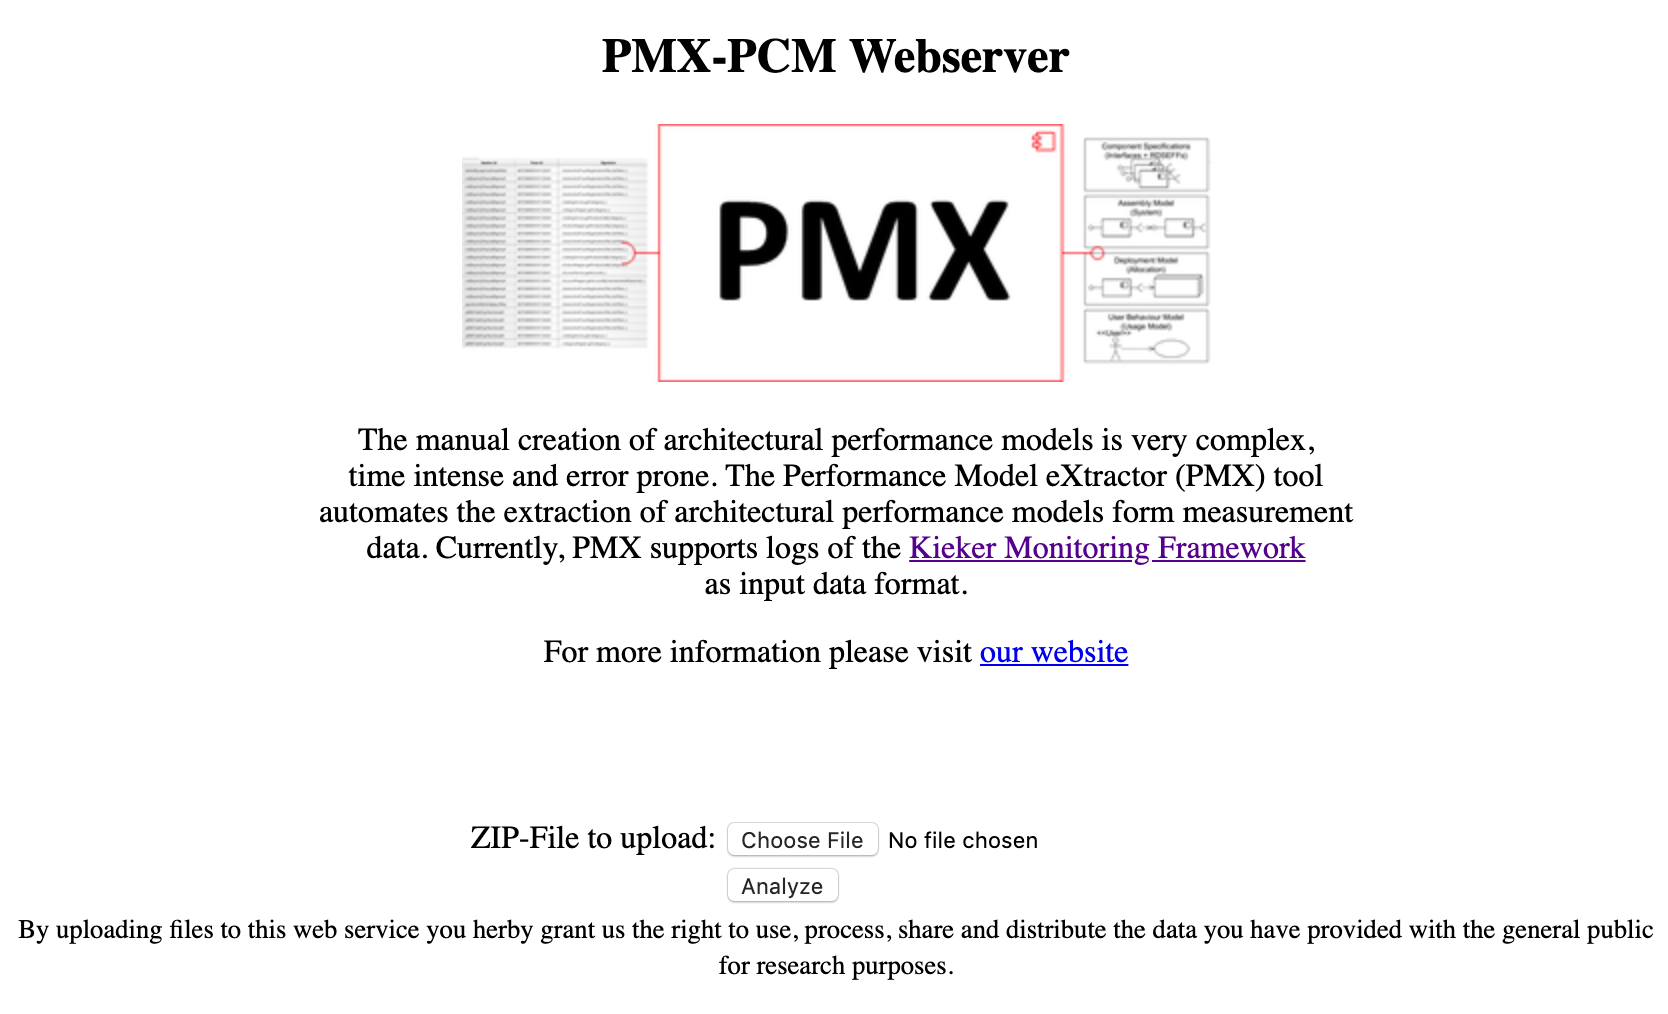
\includegraphics[width=15cm]{pcmserver}
  \caption{PMX-PCM Server. Tomado del Sitio Web de PMX}
  \label{fig:pcmserver}
\end{figure}

La figura \ref{fig:pcmserver} muestra el formulario proporcionado por el PCX-PCM WebServer para extraer un modelo PCM a partir de una bitácora en Kieker.

\subsection{Extracción con \texttt{pcmConsole.jar}} Al momento de escribir este documento \texttt{pcmConsole.jar} se encuentra bajo la siguiente ruta (suponemos ``\texttt{pmx}'' como el directorio padre, el directorio principal de la distribución descargada de \texttt{pmx}):
\begin{verbatim}
pmx/pmx-pcm/tools.descartes.pmx.pcm.docker/pcmserver/pcmConsole.jar
\end{verbatim}
Una vez dentro del directorio \texttt{pcmserver}, se puede ejecutar el siguiente comando:

\begin{verbatim}
java -jar pcmConsole.jar -i <ruta-directorio-de-bitacora> \
    -o <ruta-directorio-destino>
\end{verbatim}

\subsubsection{Consideraciones}
Si PMX no entrega ningún resultado como parte del proceso de extracción, esto quiere decir que la bitácora proporcionada no tiene un formato apropiado para PMX. Si esto pasa, vale la pena revisar los puntos en donde se introdujo la instrumentación de Kieker. Se debe revisar si los eventos contienen toda la información necesaria de acuerdo con el manual de usuario. 

\subsection{Importar archivos producidos por \texttt{PMX} a \emph{Palladio Workbench}}
\begin{singlespace}
\begin{algorithm}[H]
\SetAlgoLined
%\KwResult{Write here the result }
% initialization\;
\tcc{Se supone que se logrado obtener un modelo PCM por medio de PMX}
Crear nuevo proyecto en \emph{Palladio Workbench}\;
Importar archivos generados por \texttt{PMX}\;
\eIf{archivos son compatibles con Palladio Workbench}{
    Iniciar con la ejecución de simulaciones\;
}{
    Evaluar incompatibilidades y corregir\;
}
\caption{How to write algorithms}
\end{algorithm}
\end{singlespace}

Si el proceso anterior se realizó con éxito, PMX  generará 5 archivos en formato XML que representan cada uno de los modelos con los que se puede trabajar en Palladio: modelo de componentes, asignación de recursos, ambiente, sistema y uso. También se generan archivos \texttt{*.csv} con estimaciones del uso de los componentes. El uso de las estimaciones contenidas en estos archivos es opcional, puesto que en la Sección X explicamos una alternativa que nos brindó mayor precisión.

En \emph{Palladio Workbench} hay que crear un nuevo proyecto y ponerle un nombre.
\begin{verbatim}
File > New > Project > Other > New Palladio Project
\end{verbatim}
Luego de esto hay que importar cada uno de los archivos XML producidos por PMX al proyecto recién creado.
\begin{verbatim}
Seleccionar el proyecto > 
File > Import > File System > Seleccionar el directorio con los archivos
\end{verbatim}
Con los archivos cargados en el proyecto, se puede entonces iniciar la ejecución de simulaciones.
\begin{verbatim}
Seleccionar el proyecto > Click derecho > Run As > Run Configurations
\end{verbatim}
Luego se muestra la pantalla en donde se crean y administran configuraciones de ejecución. En este estudio se utilizó el motor de simulación \texttt{SimuBench} pero se proveen otros motores de simulación. Se puede utilizar los valores por defecto en un inicio y, por último, ejecutar las simulaciones.


\subsubsection{Consideraciones}
\begin{enumerate}
    \item Los espacios de nombres, \emph{namespaces}, de los archivos XML producidos por PMX pueden llegar a ser diferentes a los de la versión de \emph{Palladio Workbench} que se esté utilizando. Dependiendo del modelo PCM con el que se esté trabajando esto podría llegar a ser un problema. 
    \item Algunos tipos de datos producidos en los archivos XML de PMX pueden llegar a ser diferentes a los de la versión de \emph{Palladio Workbench}.
\end{enumerate}

Un ajuste que ayudó a resolver estos problemas de compatibilidad, fue generar un nuevo proyecto en \emph{Palladio Workbench} y utilizar, por ejemplo, en el modelo de repositorio, componentes similares a los producidos por PMX. Luego ver el código XML del modelo de repositorio y comparar las definiciones de este archivo con el de PMX.
 
\subsection{Refinamientos sobre el modelo}
\begin{singlespace}
\begin{algorithm}[H]
\SetAlgoLined
%\KwResult{Write here the result }
% initialization\;
\tcc{Se supone que se cuenta con modelo PCM válido}
Ejecutar simulaciones con \emph{SimuBench}\;
\Repeat{hasta que los resultados sean satisfactorios}{
    Modificar submodelos\;
    Obtener estimaciones de herramientas alternas a \texttt{PMX}\;
    Evaluar resultados\;
}
\caption{How to write algorithms}
\end{algorithm}
\end{singlespace}

Una vez que se cuenta con el modelo PCM, se puede iniciar la ejecución de simulaciones. Conforme se van dando las ejecuciones, el motor de simulaciones de PCM (en este caso SimuBench) entrega 6 tipos de visualización de resultados para cada uno de los componentes identificados. También incluye estimaciones de la demanda del procesador y el disco duro. En este trabajo fueron de particular utilidad las visualizaciones de resultados de tipo: \texttt{XP Plot}, histograma y función de distribución acumulada.

Los resultados entregados por el motor de simulaciones vienen dados en tiempos de respuesta en segundos. En el caso en el que los resultados de las simulaciones muestren resultados muy alejados a los observados en invocaciones reales, se recomienda modificar el modelo en alguno de sus submodelos asociados. Una de las desventajas que se experimentó con el modelo obtenido por PMX fueron las estimaciones de las demandas de los recursos, esto se explica con mayor detalle en la Sección \ref{sec:experimento-1}, y para lidiar con esto, fue necesario hacer uso de herramientas alternas con el fin de afinar estas estimaciones, para luego repetir las simulaciones hasta que los resultados obtenidos se consideraron relevantes. En este estudio, la herramienta AWS X-Ray fue sumamente útil para llevar a cabo esta labor. También se realizaron modificaciones sobre el modelo de uso para generar cargas de trabajo con compartamientos similares a los hechos en las invacaciones reales.

La Sección \ref{sec:experimento-1} brinda un mayor detalle acerca de la estrategia de afinamiento del modelo de rendimiento para el caso de \emph{Image Handler}, pero en términos generales, una vez obtenido un modelo, todo dentro del mismo está sujeto a modificación y evaluación. La literatura consultada hace énfasis en esto y, para el caso de \emph{Image Handler} esto no fue la excepción. Llegado a este punto, se entra en un ciclo de prueba $\rightarrow$ validación $\rightarrow$ afinamiento del modelo hasta que los resultados obtenidos por medio de las simulaciones resulten significativas para el caso de estudio en particular.



\chapter{Conclusiones}
\label{cap:conclusiones}
En esta tesis se exploró el modelado y la simulación basados en componentes sobre funciones en la nube en plataformas \emph{FaaS}, con el fin de evaluar si la aplicación de este método logra entregar información relevante sobre el comportamiento de la función, la cual pueda servir tanto para razonar sobre el diseño e implementación de la arquitectura del software, como también para tener criterios más informados para predecir el comportamiento en ambientes de producción.

Para la realización de este trabajo, se desarrolló e instaló una función Lambda en el servicio AWS Lambda.  Se utilizó una adaptación del enfoque de ingeniería de rendimiento declarativo descrito en \cite{Walter:2018:TDP:3185768.3185777} ya que, al estar haciendo los primeros pasos en el campo de la ingeniería de rendimiento de software, dicho enfoque permitió automatizar gran parte del proceso.

El principal hallazgo obtenido durante la realización de la investigación reportada en esta tesis es que el modelado y la simulación basados en componentes sí logran caracterizar en gran medida el comportamiento de una función en la nube. Luego de la ejecución de miles de invocaciones a la función en la nube y miles de simulaciones sobre el modelo de rendimiento, se pudo corroborar que los conjuntos de resultados obtenidos en ambos escenarios presentaron tendencias muy similares, lo cual fue comprobado estadísticamente. 

La instrumentalización hecha en el código fuente para soportar el monitoreo de los eventos al interior de la función causó que las simulaciones reportaran una diferencia media de 247ms con respecto del tiempo promedio de los tiempos de respuesta de las invocaciones hechas a la función Lambda.

\subsection{Análisis de resultados}
\paragraph{Experimento \#1} El primer experimento de la Sección \ref{sec:experimento-1} estuvo dirigido a generar un modelo de rendimiento a partir de las bitácoras de la función \emph{Image Handler}. Para esto, se implementó una versión de la función que fue instrumentalizada con la biblioteca de Kieker a fin de generar una bitácora en donde registrar los datos del rendimiento de los eventos asociados a la entrada, obtención de la imagen, redimensionamiento y salida de la función. Luego, se tomó dicha bitácora, que fue pasada a PMX para extraer un modelo de rendimiento en formato PCM. 

Una vez obtenido el modelo de rendimiento, se procedió a crear tres experimentos en donde se realizaron mil invocaciones de redimensionamiento sobre tres grupos de imágenes y, al mismo tiempo, se realizaron refinamientos en los componentes del modelo de rendimiento para reflejar los cambios en la demanda de la función para ejecutar mil simulaciones en \emph{Palladio Workbench}.

Finalmente, se compararon los resultados de las invocaciones reales de redimensionamiento con los de los de las simulaciones, las cuales pudieron caracterizar el comportamiento de la función Lambda con un error máximo del 1\%.

\paragraph{Experimento \#2} El experimento de la Sección \ref{sec:experimento-2} fue planteado para explorar el comportamiento de la función Lambda cuando esta era ejercitada durante un periodo continuo y, al mismo tiempo, evaluar si el modelo de rendimiento obtenido en el experimento \#1 podría explicar algo del comportamiento observado aquí.

Se ejecutaron ráfagas de mil invocaciones de redimensionamiento secuenciales utilizando imágenes aleatorias y otras ráfagas de mil invocaciones utilizando una imagen fija. Las invocaciones se realizaron sobre los tres mismos grupos de imágenes definidos en el experimento \#1.

Como resultado de la ejecución de las mil ráfagas se pudo notar con mayor detalle cómo la función Lambda arranca inicialmente en un estado ``frío'' y, conforme va recibiendo invocaciones, va pasando paulatinamente a un estado ``caliente'', como lo señalaba la literatura consultada. Al contrastar los resultados de este experimento con el modelo de rendimiento obtenido del experimento \#1, se observó que hay una relación entre las simulaciones que reportaron los tiempos de respuesta más prolongados con los tiempos de respuesta de la función cuando se encontraba en estado ``frío''. Asimismo, los tiempos de respuesta promedio de las simulaciones concuerdan con los tiempos de respuesta promedio de la función en estado ``caliente''.

\paragraph{Experimento \#3} Descrito en la Sección \ref{sec:experimento-3}, es una variante del experimento \#2. Se introdujeron tiempos de inactividad entre ráfagas de invocaciones de redimensionamiento y, como en el experimento \#2, se buscó evaluar el comportamiento de la función ante estas ráfagas y la posible relación de este comportamiento con el modelo de rendimiento.

Se ejecutaron ráfagas de cien invocaciones de redimensionamiento y se introdujeron tiempos de inactividad de 10, 20, 40 y 80 minutos entre cada ráfaga. Se utilizaron los mismos tres grupos de imágenes del experimento \#1 en las invocaciones de redimensionamiento.

Conforme se fue incrementando el tiempo de inactividad entre ráfagas, observamos un incremento también en la posibilidad de que la función cayera en un estado ``frío'' y, aunque este comportamiento no fue introducido explícitamente en el modelo de rendimiento, sí se pudo notar una correspondencia entre los tiempos de respuesta de la función Lambda en estado ``frío'' y ``caliente'' en las ráfagas individuales con los resultados de las simulaciones.

\paragraph{Experimento \#4} En este experimento se puso a prueba la herramienta \texttt{SAM CLI} para determinar su confiabilidad para simular y tener algún grado de predicción del comportamiento de una función Lambda en un ambiente de producción (en este caso AWS Lambda). 

Para explorar esto, se realizaron mil invocaciones de redimensionamiento en cada una de las dos plataformas, de manera que las secuencias de imágenes por redimensionar fueran idénticas en ambos casos. Los resultados de las invocaciones demostraron que el comportamiento en \texttt{SAM CLI} resultó ser muy diferente al de AWS Lambda y, al menos para el caso de \emph{Image Handler}, no resultó ser de utilidad para obtener una estimación de la ejecución de la función en un ambiente de producción.

\subsection{Cumplimiento de objetivos}
A continuación se dan a conocer las actividades que se llevaron a cabo para cumplir con los objetivos específicos planteados para esta tesis:

%    \item Revisar el estado del arte de trabajos relacionados con enfoques de predicción y medición del rendimiento en sistemas de software como servicio.\label{sec:obj1}
%    \item Sintetizar un caso de uso de una función en la nube considerada como de referencia, con el propósito de analizar su comportamiento.\label{sec:obj2}
%    \item Elaborar, conforme a un diseño experimental, pruebas de rendimiento sobre el caso de uso seleccionado a fin de obtener datos base.
%    \item Analizar los datos experimentales mediante herramientas de extracción de modelos de rendimiento de software.
%    \item Proponer y validar modelos de rendimiento a partir de los experimentos realizados.        
%    \item Formular una guía metodológica para dar a conocer aspectos de rendimiento en funciones en la nube a partir de la experiencia obtenida.

\paragraph{Objetivo \#\ref{sec:obj1}:} \emph{Revisar el estado del arte de trabajos relacionados con enfoques de predicción y medición del rendimiento en sistemas de software como servicio.}\\
En el Capítulo \ref{cap:antecedentes} se presenta una revisión de literatura de estudios relacionados con el modelado de rendimiento de software, retos y oportunidades de investigación que existen en esta área.

\paragraph{Objetivo \#\ref{sec:obj2}} \emph{Sintetizar un caso de uso de una función en la nube considerada como de referencia, con el propósito de analizar su comportamiento}.\\
Se desarrolló la función Lambda \emph{Image Handler}, que permite el redimensionamiento de imágenes ``al vuelo'' y que es considerada como un caso de uso de referencia en AWS. Los detalles de la implementación de esta función Lambda se abarcan en el Capítulo \ref{cap:manejador-imagenes}.
 
\paragraph{Objetivo \#\ref{sec:obj3}} \emph{Elaborar, conforme a un diseño experimental, pruebas de rendimiento sobre el caso de uso seleccionado a fin de obtener datos base.}\\
En los cuatro experimentos planteados en el Capítulo \ref{cap:diseno-experimental}, se realizaron pruebas de rendimiento utilizando tres grupos de imágenes sobre la función Lambda. Los resultados obtenidos a partir de estas pruebas permitieron obtener datos base sobre el rendimiento de la función y hacer comparaciones con los resultados de las simulaciones posteriores.

\paragraph{Objetivo \#\ref{sec:obj4}} \emph{Analizar los datos experimentales mediante herramientas de extracción de modelos de rendimiento de software.}\\
En las Secciones \ref{sec:estrategia-de-extraccion-de-modelo} y \ref{sec:experimento-1} se expone la estrategia y la aplicación de extracción y obtención de un modelo de rendimiento a partir de datos experimentales. En la Sección \ref{sec:estrategia-de-extraccion-de-modelo} se da a conocer la estrategia general para la extracción y obtención de un modelo de rendimiento, la cual, como ahí mismo se indica es una variante del enfoque de ingeniería de rendimiento declarativo propuesto en \cite{Walter:2018:TDP:3185768.3185777}.

Como parte de las tareas realizadas en el experimento llevado a cabo en la Sección \ref{sec:experimento-1} se:
\begin{itemize}
    \item implementaron variantes de la función Lambda a las cuales se les ejecutaron pruebas de rendimiento, que fueron de mucha utilidad para calibrar el modelo de rendimiento obtenido.
    \item se obtuvieron bitácoras con datos del rendimiento de estas funciones Lambda alternativas y
    \item se analizaron las bitácoras y se extrajo un modelo de rendimiento por medio de la herramienta PMX.
\end{itemize}


\paragraph{Objetivo \#\ref{sec:obj5}} \emph{Proponer y validar modelos de rendimiento a partir de los experimentos realizados.}\\
A partir del modelo de rendimiento obtenido, se inició un ciclo de prueba $\rightarrow$ validación $\rightarrow$ afinamiento. Estas actividades se exponen con mayor detalle en la descripción del experimento de la Sección \ref{sec:experimento-1}.

Se ejecutaron simulaciones sobre el modelo y se validaron los resultados contra los obtenidos en la función Lambda base IM-Simple. Se llevaron a cabo cálculos estadísticos para evaluar cuán similares eran ambos conjuntos de resultados.

En los experimentos de las Secciones \ref{sec:experimento-2}, \ref{sec:experimento-3} y \ref{sec:experimento-4}, se tomó el modelo de rendimiento como referencia para comparar los resultados obtenidos de cada experimento con los resultados de las simulaciones sobre el modelo con el fin de explorar las relaciones entre uno y otro.

\paragraph{Objetivo \#\ref{sec:obj6}} \emph{Formular una guía metodológica para dar a conocer aspectos de rendimiento en funciones en la nube a partir de la experiencia obtenida.}\\
La guía metodológica del Capítulo \ref{cap:guia-metodologica} expone las actividades que se llevaron a cabo para la obtención de un modelo de rendimiento a partir de una función Lambda. Se espera que lo expuesto en esta guía sirva como un punto de partida para explorar las herramientas y los enfoques utilizados en este trabajo y, de esta manera, replicarlos o extenderlos en otros casos de uso.

\subsection{Trabajo futuro}
Conforme se fue desarrollando esta tesis se fueron reconociendo aspectos que ameritan ser profundizados en aras de crear mayor conocimiento el área del modelado y la simulación basados en componentes y arquitecturas o aplicaciones en ambientes en la nube.

La lista que se presenta a continuación sintetiza los temas identificados como relevantes para ser profundizados:
\begin{itemize}
    \item \emph{Estudios sobre el rendimiento de funciones en la nube instaladas en plataformas FaaS \emph{Open Source}}: el trabajo de esta tesis se llevó a cabo en la plataforma AWS Lambda, una plataforma propietaria. Si se replicara este estudio en plataformas FaaS \emph{Open Source}, se podría evaluar si el método aquí presentando puede llevarse a cabo en tales ambientes.
    \item \emph{Estudios sobre ingeniería de rendimiento aplicados en ambientes en la nube en general:} este fue uno de los principales retos reportados en la literatura consultada. A pesar de la popularidad creciente de este modelo de computación, no existen muchos estudios asociados a arquitecturas de software 
    \item \emph{Evaluación del rendimiento de las plataformas FaaS por medio de modelado y simulación}: alternativamente, se reconoce valor en examinar el comportamiento de toda una plataforma FaaS por medo de modelado y simulación. Para llevar a cabo este estudio se podría utilizar plataformas FaaS \emph{Open Source} como Apache OpenWhisk. Tal estudio podría brindar mayores detalles de las particulares del comportamiento de la plataforma FaaS y cómo esta interactúa e impacta con el rendimiento de funciones en la nube.
    \item \emph{Extensión del Palladio Workbench para incluir componentes propios para modelado y simulación de aplicaciones en ambientes en la nube}: \emph{Palladio Workbench} está diseñado para el modelado y simulación de software de uso general, por lo que las particulares de las arquitecturas de software en ambientes en la nube no se incluyen. Estas deben ser incluidas de formas explícita e interpretadas con los motores de simulación y visualización con lo que pone a disposición la herramienta. Nuevos componentes para análisis de arquitecturas en la nube en \emph{Palladio Workbench} contribuirían a promover el estudio de carácterísticas de rendimiento, escalabilidad e integración, áreas en las que se ha reportado que existe una necesidad.
    \item \emph{Desarrollo de herramientas para implementación y prototipado de funciones en la nube que tomen en cuenta las particularidades de la instalación y la ejecución en ambientes de producción}: actualmente las herramientas existentes son competentes pero no brindan mayor información sobre la ejecución de las funciones en un eventual ambiente de producción. Esto es importante porque ayudaría a calibrar aún más los aspectos relacionados con la arquitectura y el rendimiento antes que se llegue a dar la instalación.
\end{itemize}

\subsection{Sobre las herramientas de modelado y simulación utilizadas en este estudio}
Kieker, PMX y \emph{Palladio Workbench} fueron las principales herramientas para generar bitácoras de un sistema, extracción de modelos, simulación y visualización de resultados. De las tres, \emph{Palladio Workbench} es la que cuenta tanto con una trayectoria más amplia en el área de la ingeniería de rendimiento de software así como de un grupo de trabajo más activo que está periódicamente lanzando nuevas versiones del producto. Esta herramienta fue probada en estudios preliminares por el autor y esto contribuyó a familiarizarse en la forma en la que esta trabaja.

La adopción y el uso de Kieker y PMX fue algo totalmente nuevo pero, gracias al hecho de que ambas son herramientas estables y que cuentan con una documentación actualizada, la curva de aprendizaje fue baja y se logró que ambas se pudieran integrar con el código existente.

Estas tres herramientas tienen una orientación más académica que comercial por lo que se recomienda ser precavido en su adopción y uso ya que, a pesar que las universidades que las desarrollan han demostrado mantener un desarrollo activo a lo largo de los años, estas podrían dejar de ser mantenidas o no funcionar bajo un escenario en particular. Se recomienda la lectura de la guía metodológica de la Sección \ref{cap:guia-metodologica} para obtener mayores detalles de la forma sobre la que se utilizaron dichas herramientas en este estudio.

\subsection{Reflexiones personales}
En principio, si bien la propuesta de este estudio se presentaba como un reto, se sabía también que había mucho valor en trabajar en esto y poder aportar a esta área de conocimiento. Durante todo este proceso fui alentado por mi profesor tutor Ignacio Trejos y, gracias a su invaluable colaboración, se pudo dar forma a este documento y reportar los hallazgos obtenidos.

En muchas tareas retadoras que se presentan en la vida es difícil medir su complejidad sin antes trabajar en ellas, considero que la realización de una tesis es un ejemplo de esto: en necesario empezar y ser constante con el fin de ahondar en el tema y resolver los problemas que se van dando.

El camino que he recorrido durante el Programa de Maestría en Computación ha sido fascinante y sumamente enriquecedor. He tenido la oportunidad de aprender, conocer nuevas personas y ser mejor. Esto es algo que voy agradecer por siempre al equipo de trabajo del Programa de Maestría y en especial a los profesores con los que tuve el privilegio de ser alumno.

%
%\chapter{Antecedentes}
%\label{cap:antecedentes}
%\section{Marco conceptual}

\subsection{Ingeniería de rendimiento de software (\emph{Software Performance Engineering})}
Una descripción comúnmente utilizada para definir ingeniería de rendimiento de software  (\emph{Software Performance Engineering} - SPE)  es la brindada en Woodside et al. \cite{4221619}: \textit{``Ingeniería de rendimiento del software representa toda la colección de actividades de ingeniería de software y análisis relacionados utilizados a través del ciclo de desarrollo de software que están dirigidos a cumplir con los requerimientos de rendimiento''}. 

De acuerdo con estos mismos autores, los enfoques para ingeniería de rendimiento puede ser divididos en dos categorías: basadas en mediciones y basadas en modelos. La primera es la más común y utiliza pruebas, diagnóstico y ajustes una vez que existe un sistema en ejecución que se puede medir; es por esto que solamente puede ser utilizada conforme se va acercando el final del ciclo de desarrollo de software. En contraste con el enfoque basado en mediciones, el enfoque basado en modelos se centra en las etapas iniciales del desarrollo. Como el nombre lo indica, en este enfoque los modelos son clave para hacer predicciones cuantitativas de cuán bien una arquitectura puede cumplir sus expectativas de rendimiento.

Se han propuesto otras clasificaciones de enfoques para SPE pero, con respecto de la evaluación de sistemas basados en componentes, en \cite{Koziolek:2010:PEC:1808359.1808729} se deja la clasificación a un lado debido a que se argumenta que la mayoría de enfoques de modelaje toman alguna medición como entrada y a la mayoría de los métodos de medición los acompaña algún modelo.

\subsubsection{Ingeniería de rendimiento basada en mediciones}
Los enfoques basados en mediciones son los que prevalencen en la industria\cite{Gooijer2011PerformanceMO} y son típicamente utilizados para verificación(¿cumple el sistema con sus requerimientos de rendimiento?) o para localizar y reparar \emph{hot-spots} (cuáles son las partes que tienen peor rendimiento en el sistema). La medición de rendimiento se remonta al inicio de la era de la computación, lo que ha generado una amplia gama de herramientas como generadores de carga y monitores para crear cargas de trabajo ficticias y llevar a cabo la medición de un sistema respectivamente.

Las pruebas de rendimiento aplican técnicas basadas en medición y usualmente esto es hecho luego de las pruebas funcionales o de carga. Las pruebas de carga validan el funcionamiento de un sistema bajo cargas de trabajo pesadas, mientras que las pruebas de rendimiento son usadas para obtener datos cuantitativos de características de rendimiento, como tiempos de respuesta, \emph{throughput} y utilización de hardware para una configuración de un sistema bajo una carga de trabajo definida.

\subsubsection{Ingeniería de rendimiento por medio de modelado} 
La importancia del modelado del rendimiento está motivada por el riesgo de que se presenten problemas graves de rendimiento y la creciente complejidad de sistemas modernos, lo que hace difícil abordar los problemas de rendimiento en el nivel de código\cite{Reussner:2016:MSS:3036121}. Cambios considerables en el diseño o en las arquitecturas pueden ser requeridos para mitigar los problemas de rendimiento. Por esta razón, la comunidad de investigación de modelado de rendimiento intenta luchar contra el enfoque de ``arreglar las cosas luego'' durante el proceso de desarrollo. Con la aplicación de un modelo del rendimiento de software se busca encontrar problemas de rendimiento y alternativas de diseño de manera temprana en el ciclo de desarrollo, evitando así el costo y la complejidad de un rediseño o cambios en los requerimientos.

Las herramientas de modelado de rendimiento ayudan a predecir la conducta del sistema antes que este sea construido, o bien, evaluar el resultado de un cambio antes de su implementación. El modelado del rendimiento puede ser usado como una herramienta de alerta temprana durante todo el ciclo de desarrollo con mayor precisión y modelos cada vez más detallados a lo largo del proceso. Al iniciar el desarrollo, un modelo no puede ser validado contra un sistema real, por esto el modelo representa el conocimiento incierto del diseñador. Como consecuencia de esto el modelo incluye suposiciones que no necesariamente se van a dar en el sistema real, pero que van a ser útiles para obtener una abstracción del comportamiento del sistema. En estas fases iniciales, la validación se obtiene mediante el uso del modelo, y existe el riesgo de conclusiones erróneas debido a su precisión limitada. Luego, el modelo puede ser validado contra mediciones en el sistema real (o parte de este) o prototipos de este, lo cual hace que la precisión del modelo se incremente.

En \cite{Jin:2007:PEP:1248820.1248885} se sugiere que los métodos actuales deben superar diversos retos antes de poder aplicarlos en sistemas existentes que enfrentan cambios en su arquitectura o requerimientos. Primero, debe quedar claro cómo se obtienen los valores para los parámetros del modelo y cómo se pueden validar los supuestos. Estimaciones basadas en la experiencia para estos parámetros no son suficientes, por lo que es necesario hacer mediciones en el sistema existente para formular predicciones precisas. Segundo, la caracterización de la carga del sistema en un entorno de producción es problemática debido a los recursos compartidos (bases de datos, hardware). Tercero, deben desarrollarse métodos para capturar parámetros del modelo dependientes de la carga. Por ejemplo un incremento en el tamaño de la base de datos probablemente incrementará las necesidades de procesador, memoria y disco en el servidor.

Técnicas comunes de modelado incluyen redes de colas y también extensiones de estas como redes de colas en capas y varios tipos de redes de Petri, y álgebras de procesos estocástica.

\subsubsection{Modelado de Rendimiento}
En SPE, la creación y evaluación de modelos de rendimiento es un concepto clave para evaluar cuantitativamente el rendimiento del diseño de un sistema y predecir el rendimiento de diversas alternativas de diseño. Un modelo de rendimiento captura el comportamiento relevante de diversos elementos (y sus interacciones) para identificar el efecto de cambios en la configuración o en la carga de trabajo sobre el rendimiento de un sistema. Un buen modelo permite predecir los efectos de tales cambios sin necesidad de implementar y ejecutar un sistema en un ambiente de producción, que podrían ser no solamente tareas costosas sino también un desperdicio en caso que el hardware con el que se cuenta demuestre ser insuficiente para soportar la intensidad de la carga de trabajo.\cite{Noorshams2015_1000046750}

La forma del modelo de rendimiento puede comprender desde funciones matemáticas a formalismos de modelado estructural y modelos de simulación. Estos modelos varían en sus características clave; por ejemplo, los supuestos de modelado de los formalismos, el esfuerzo de modelado requerido y el nivel de abstracción.

En cuanto a técnicas de simulación, a pesar que estas permiten un estudio más detallado de los sistemas que modelos analíticos, la construcción de un modelo de simulación requiere de conocimiento detallado tanto de desarrollo de software como de estadística\cite{Gooijer2011PerformanceMO}. Los modelos de simulación también requieren usualmente de mayor tiempo de desarrollo que los modelos analíticos. En \cite{4221619} se menciona que ``la construcción de un modelo de simulación es cara, algunas veces comparable con el desarrollo de un sistema, y, los modelos de simulación detallados puede tardar casi tanto en ejecutarse como el sistema''.

\subsection{Modelado y simulación de rendimiento basado en componentes}
En este enfoque, modelos clásicos de rendimiento tales como redes de colas, redes de Petri estocásticas o álgebras de procesos estócasticas son aplicadas para modelar y analizar el rendimiento de software basado en componentes. La ingeniería de software basada en componentes se considera un sucesor del desarrollo de software orientado a objetos, en esta los componentes de software son unidades de composición a las que se le define una especificación y una interfaz. A partir de estas, los arquitectos de software construyen e integran componentes de software entre sí, creando de esta manera sistemas más complejos.\cite{Koziolek:2010:PEC:1808359.1808729}

El reto en los modelos de rendimiento para componentes, es que el rendimiento de un componente de software en un sistema en ejecución depende del contexto en que está instalado y su perfil de uso, el cual es usualmente desconocido por el desarrollador del componente que creal el modelo de un componente individual.

\subsubsection{Rendimiento de componentes de software}
Szyperski\cite{Szyperski:2002:CSB:515228} define un componente de software como: \textit{``Un componente es una unidad de composición en aplicaciones de software, que posee un conjunto de interfaces y un conjunto de requerimientos (una especificación), y que ha de poder ser desarrollado, adquirido, incorporado al sistema y compuesto con otros componentes de forma independiente, en tiempo y espacio''}. 

Los componentes de software presentan los principios de ocultación de la información y la separación de responsabilidades. Fomentan la reutilización y preparan el sistema para que se puedan efectuar cambios de partes individuales. Permiten además una división de trabajo entre los desarrolladores de componentes y los arquitectos de software, lo que reduce la complejidad de la tarea de desarrollo. Los componentes de caja negra (\emph{black-box}) solamente revelan sus interfaces a los clientes, mientras que los componentes de caja blanca (\emph{white-box}) permiten ver y modificar el código fuente de la implementanción del componente como tal. Los componentes compuestos agrupan varios componentes en unidades más grandes.

\paragraph{Factores que influyen en el rendimiento de un componente}
Especificar el rendimiento de componentes reutilizables es difícil porque esto no solamente va a depender de la implementación del componente, sino también del contexto en donde este se encuentre instalado. Los factores que influyen en el rendimiento de los componentes son:

\begin{figure}[h]
  \centering
  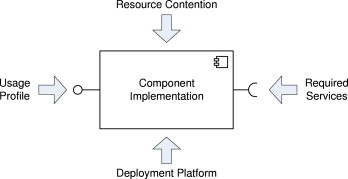
\includegraphics[width=10cm]{component-performance}
  \caption[Factores que influyen en el rendimiento de un componente]{Factores que influyen en el rendimiento de un componente. Tomado de \protect\cite{Koziolek:2010:PEC:1808359.1808729}}
  \label{fig:component-performance}
\end{figure}

\begin{itemize}
    \item \emph{Implementación del componente}: los desarrolladores pueden implementar la funcionalidad especificada en una interfaz de diferentes formas. Dos componentes pueden proporcionar el mismo servicio pero presentar tiempos de ejecución diferentes cuando se ejecutan con los mismos recursos y con las mismas entradas.
    \item \emph{Servicios requeridos}: cuando el componente $A$ invoca el servicio del componente $B$, el tiempo de ejecución de $B$ suma al tiempo de ejecución de $A$. Por lo tanto, el tiempo total de ejecución de un componente depende del tiempo de ejecución de los otros componentes/servicios que necesita.
    \item \emph{Plataforma de instalación}: los arquitectos de software instalan un componente de software en diferentes plataformas. Una plataforma de instalación puede incluir varias capas de software (como por ejemplo contenedores de componentes o máquinas virtuales) y hardware (procesador, dispositivos de almacenamiento y red, etc)
    \item \emph{Perfil de uso}: clientes pueden invocar los servicios del componente con diferentes parámetros de entrada. El tiempo de ejecución de un servicio puede cambiar dependiendo de los valores de lo parámetros de entrada.
    \item \emph{Contención de recursos}: un componente de software típicamente no se ejecuta como un solo proceso aislado en una plataforma determinada. Los tiempos de espera inducidos para acceder a recursos limitados se suman al tiempo de ejecución de un componente de software.
\end{itemize}

\subsubsection{Enfoques de ingeniería de rendimiento para software basado en componentes propuestos}
La encuesta llevada a cabo en \cite{Koziolek:2010:PEC:1808359.1808729} proporciona una clasificación de enfoques de medición y predicción de rendimiento para sistemas de software basados en componentes. Otra clasificación es la que se expone en \cite{1291833}, donde se presenta una revisión de métodos de predicción de rendimiento basado en modelos para sistemas en general, pero no analiza los requerimientos propios para sistemas basados en componentes. 

De acuerdo con \cite{Koziolek:2010:PEC:1808359.1808729} durante los últimos diez años, los investigadores han propuesto muchos enfoques para evaluar el rendimiento (tiempos de respuesta, \emph{throughput}, utlización de recursos) de sistemas de software basados en componentes. Estos enfoques abarcan tanto predicción como medición del rendimiento. Los primeros analizan el rendimiento esperado de un diseño de software basado en componentes para evitar problemas de rendimiento en la implementación del sistema, lo que podría llevar a costos substanciales para rediseñar la arquitectura. Los otros analizan el rendimiento observable de sistemas de software basados en componentes implementados para entender sus propiedades, determinar su capacidad máxima, identificar componentes críticos y para resolver cuellos de botella.

\paragraph{Métodos de evaluación de rendimiento}
Los enfoques se reunieron en dos grandes grupos: enfoques principales que proporcionan procesos de evaluación de rendimiento completo y enfoques suplementarios que se centran en aspectos específicos como medición de componentes individuales o modelaje de las propiedades de rendimiento de los conectores de un componente.

\paragraph{Enfoques principales}
\begin{itemize}
    \item \textbf{Enfoques de predicción basados en UML}: los enfoques en este grupo se enfocan en la predicción de rendimiento en tiempo de diseño para sistemas de software basado en componentes modelados con el Lenguaje de Modelado Unificado (UML por sus siglas en inglés). UML 2.0 tiene la noción de componente de software como una clase extendida. UML permite modelar el comportamiento de un componente con diagramas de secuencia, actividad y colaboración. La asignación de los componentes puede ser descrita mediante diagramas de despliegue(\emph{deployment}).     
%    Mientras que UML solamente soporta especificaciones funcionales, su mecanismo de extensión (perfiles que consisten de estereotipos, restricciones y valores etiquetados) ha sido utilizado por el \emph{Object Management Group} para permitir el modelado de atributos de rendimiento como valores de tiempo y parámetros de cargas de trabajo. 
    \begin{itemize}
        \item CB-SPE - \emph{Component-Based Software Performance Engineering} 
    \end{itemize}
    \item \textbf{Enfoques de predicción basados en Meta-Modelos propietarios}: Los enfoques en este grupo apuntan a las predicciones de rendimiento de tiempo de diseño. En lugar de usar UML como lenguaje de modelado para desarrolladores y arquitectos, estos enfoques tienen meta-modelos propietarios\cite{Koziolek:2010:PEC:1808359.1808729}.
    \begin{itemize}
        \item CBML - \emph{Component-Based Modeling Language}
        \item PECT - \emph{The Prediction Enabled Component Technology}
        \item COMQUAD - \emph{Components with Quantitative properties and Adaptivity}
        \item KLAPPER
        \item ROBOCOP
        \item Palladio        
    \end{itemize}
    \item \textbf{Enfoques de predicción centrados en \emph{middleware}}: hacen énfasis en la influencia del \emph{middleware} en el rendimiento de un sistema basado en componentes. Por lo tanto miden y modelan el rendimiento de plataformas \emph{middleware} como JavaEE o .Net. Se basan en suponer que la lógica de negocio de los componentes tiene poco impacto en el rendimiento general del sistema y por eso no requieren un modelado detallado.
    \begin{itemize}
        \item NICTA
    \end{itemize}
    \item \textbf{Enfoques basados en especificaciones formales}: estos enfoques siguen teorías fundamentales de especificación de rendimiento y no toman en cuenta marcos de trabajo (\emph{frameworks}) de medición y predicción.
    \begin{itemize}
        \item RESOLVE
        \item HAMLET
    \end{itemize}
    \item \textbf{Enfoques de monitoreo para sistemas implementados}: suponen que un sistema basado en componentes ha sido implementado y puede ser probado. El objetivo es encontrar problemas de rendimiento en un sistema en ejecución, identificar cuellos de botella y adaptar el sistema para que pueda lograr los requerimientos de rendimiento.
   \begin{itemize}
        \item COMPAS
        \item TESTEJB
        \item AQUA
        \item PAD
    \end{itemize}    
\end{itemize}
  

\paragraph{Enfoques Suplementarios}
\begin{itemize}
    \item \textbf{Enfoques de monitoreo para componentes implementados}: El objetivo de los enfoques de medición para implementaciones de componentes de software individuales es derivar especificaciones de rendimiento parametrizadas a través de mediciones múltiples. El objetivo es obtener el perfil de uso, dependencias y la plataforma de implementación a partir de la especificación de rendimiento, de modo que pueda usarse en diferentes contextos. 
    \begin{itemize}
        \item RefCAM
        \item COMAERA
        \item ByCounter
    \end{itemize}
    \item \textbf{Enfoques de predicción con énfasis en conectores de componentes}: Estos enfoques suponen un lenguaje de descripción de componentes existente y se centran en modelar y medir el impacto en el rendimiento de las conexiones entre componentes. Estas conexiones pueden implementarse con diferentes técnicas \emph{middleware}.
    \begin{itemize}
        \item Verdickt
        \item Grassi
        \item Becker
        \item Happe
    \end{itemize}        
\end{itemize}

Recientemente varios enfoques de predicción basados en meta-modelos propietarios han sido propuestos para la optimización del diseño de arquitecturas, modelado de calidad de servicio y escalabilidad. PerOpteryx\cite{Koziolek:2011:PAA:2000259.2000267} es un enfoque de optimización de diseño de arquitecturas que manipula modelos especificados en \emph{Palladio Component Model}\cite{Reussner:2016:MSS:3036121} y utiliza el algoritmo evolutivo multi-objetivo \texttt{NSGA-II}. Para análisis de rendimiento utiliza redes de colas en capas. \emph{Descartes Modeling Language}\cite{KoBrHu2014-TechReport-DML} es un lenguaje de modelado de arquitecturas para modelar calidad de servicio y aspectos relacionados con la gestión de recursos de los sistemas, las infraestructuras y los servicios de tecnología de información dinámicos modernos. \emph{CloudScale}\footnote{\url{http://www.cloudscale-project.eu/}}\cite{Brataas:2013:CSM:2479871.2479920} es un enfoque de diseño y evolución de aplicaciones y servicios escalables en la nube. En \emph{CloudScale} se identifica y gradualmente se resuelven problemas de escalabilidad en aplicaciones existentes y también permite el modelado de alternativas de diseño y el análisis del efecto de la escalabilidad en el costo. Cabe mencionar que estos últimos enfoques han sido influenciados en gran medida por el trabajo llevado a cabo en \emph{Palladio Component Model}.

\subsubsection{Modelado de Arquitecturas de Software con \emph{Palladio Component Model}} \label{sec:pcm}
El \emph{Palladio Component Model} es un enfoque de modelaje para arquitecturas de software basados en componentes que permite predicción de rendimiento basada en modelos. PCM contribuye al proceso de desarrollo de ingeniería basada en componentes y proporciona conceptos de modelaje para describir componentes de software, arquitectura de software, despliegue (\emph{deployment}) de componentes y perfiles de uso de sistemas de software basados en componentes en diferentes submodelos (Figura \ref{fig:pcm-instance}). 

\begin{figure}[h]
  \centering
  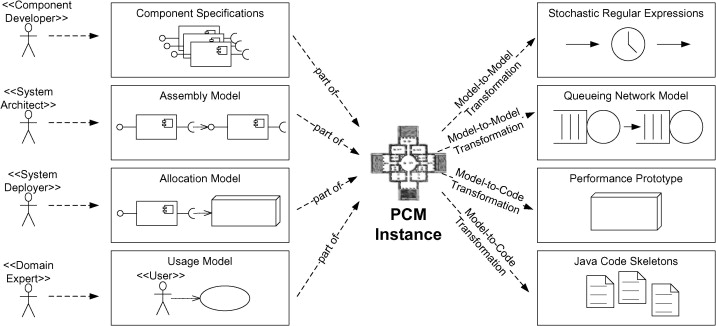
\includegraphics[width=15cm]{palladio-cbse-process}
  \caption[Instancia de un modelo PCM]{Instancia de un modelo PCM. Tomado de \protect\cite{Becker:2009:PCM:1458724.1458819}}
  \label{fig:pcm-instance}
\end{figure}

\begin{itemize}
    \item \textbf{Especificaciones de componentes} son descripciones abstractas y paramétricas de los componentes de software. En las especificaciones de software se proporciona una descripción del comportamiento interno del componente así como las demandas de sus recursos en RDSEFFs (\emph{Resource Demanding Service EFFect specifications}) utilizando una sintaxis similar a los diagramas de actividad de UML.
    \item \textbf{Un modelo de ensamblaje} (\emph{assembly model}) especifica qué tipo de componentes se utilizan en una instancia de aplicación modelada y si las instancias del componente se replican. Además, define cómo las instancias del componente se conectan, para representar la arquitectura de software.
    \item El entorno de ejecución y los recursos, así como la instalación (\emph{deployment}) de instancias de componentes para dichos contenedores de recursos se definen en un \textbf{modelo de asignación} (\emph{allocation model}).
    \item El \textbf{modelo del uso} especifica la interacción de los usuarios con el sistema utilizando una sintaxis similar al diagrama de actividades de UML, para proporcionar una descripción abstracta de la secuencia y la frecuencia con que los usuarios activan las operaciones disponibles en un sistema.
\end{itemize}

Un modelo PCM abstrae un sistema de software en el nivel de arquitectura y se anota con consumos de recursos que fueron medidos previamente y otros que son estimados. El modelo puede entonces ser usado en transformaciones de modelo-a-modelo o modelo-a-texto a un modelo de análisis en particular (redes de colas o simulación de código) que puede ser resuelto analíticamente o mediante simulación para obtener resultados sobre el rendimiento y predicciones del sistema modelado. Los resultados del rendimiento y las predicciones pueden ser utilizadas como retroalimentación para evaluar y mejorar el diseño inicial, permitiendo así una evaluación de calidad de los sistemas de software con base en un modelo\cite{Noorshams2015_1000046750}.


\subsubsection{Modelado de Arquitecturas de Software con \emph{Descartes Modeling Language}} \label{sec:dml}
El \emph{Descartes Modeling Language} (DML) es un lenguaje de modelado de nivel de arquitectura utilizado para describir calidad de servicio (\emph{QoS} por sus siglas en inglés) y aspectos relacionados con la gestión de recursos de sistemas de información dinámicos, infraestructuras y servicios. DML distingue explicítamente diferentes tipos de modelos que describen el sistema y sus procesos de adaptación desde un punto de vista técnico y lógico. Juntos, estos diferentes tipos de modelos forman una instancia DML. La idea detrás del uso de estos modelos es separar el conocimiento acerca de la arquitectura del sistema y el comportamiento de su rendimiento (aspectos técnicos), del conocimiento de los procesos de adaptación del sistema (aspectos lógicos)\cite{KoBrHu2014-TechReport-DML}.

\begin{figure}[h]
  \centering
  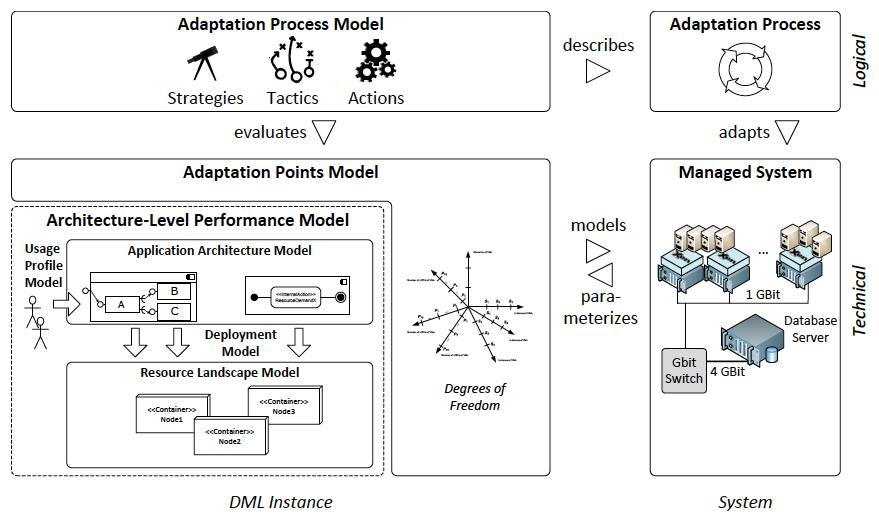
\includegraphics[width=16cm]{dml-instance}
  \caption[Relación de los diferentes modelos de una instancia DML y el sistema]{Relación de los diferentes modelos de una instancia DML y el sistema. Tomado de \protect\cite{KoBrHu2014-TechReport-DML}}
  \label{fig:dml-instance}
\end{figure}

La figura \ref{fig:dml-instance} muestra la relación de los diferentes modelos que son parte de una instancia DML, el sistema gestionado (\emph{managed system}) y el proceso de adaptación del sistema (\emph{adaptation process}). En la esquina inferior derecha de la figura \ref{fig:dml-instance}, se ve el sistema, el cual es gestionado por un proceso de adaptación, mostrado en la esquina superior derecha de la figura \ref{fig:dml-instance}. En la esquina inferior izquierda se muestran modelos que reflejan los aspectos técnicos del sistema. Esos aspectos son los recursos de hardware y su distribución (\emph{resource landscape model}), los componentes de software y el comportamiento relevante al rendimiento (\emph{application architecture model}), la instalación de componentes de software en el hardware (\emph{deployment model}), el comportamiendo del uso y las cargas de trabajo de los usuarios del sistema (\emph{usage profile model}) y los grados de libertad del sistema que pueden ser empleados para la adaptación del sistema en ejecución (\emph{adaptation points model}). Por encima de estos modelos (esquina superior izquierda de la figura \ref{fig:dml-instance}) se muestra el modelo de proceso de adaptación, que especifica un proceso de adaptación que describe cómo el sistema se adapta a cambios en su ambiente. El proceso de adaptación aprovecha las técnicas de predicción de rendimiento en línea para razonar sobre posibles estrategias, tácticas y acciones de adaptación.

\subsubsection{Enfoque de ingeniería de rendimiento declarativo}
%Las cargas de trabajo descritas en la sección \ref{sec:manejador-imagenes-spe} van a alimentar la bitácora de eventos de la función. En AWS el servicio encargado de llevar registro de los eventos que suceden en una función Lambda se llama Amazon CloudWatch\footnote{\url{https://aws.amazon.com/cloudwatch}}. 

Para obtener un modelo a partir del comportamiento de un software en existente, en Walter et al.\cite{Walter:2018:TDP:3185768.3185777} se introduce el enfoque de ingeniería de rendimiento declarativo, el cual busca la automatización de gran parte del proceso de ingeniería de rendimiento  con el fin de explorar, responder y visualizar aspectos concernientes al rendimiento de un sistema. Esto se logra gracias a una serie de herramientas desarrolladas por el grupo de ingeniería de software de la Universidad Würzburg de Alemania y que están disponibles en \url{http://descartes.tools}.

\begin{figure}[h]
  \centering
  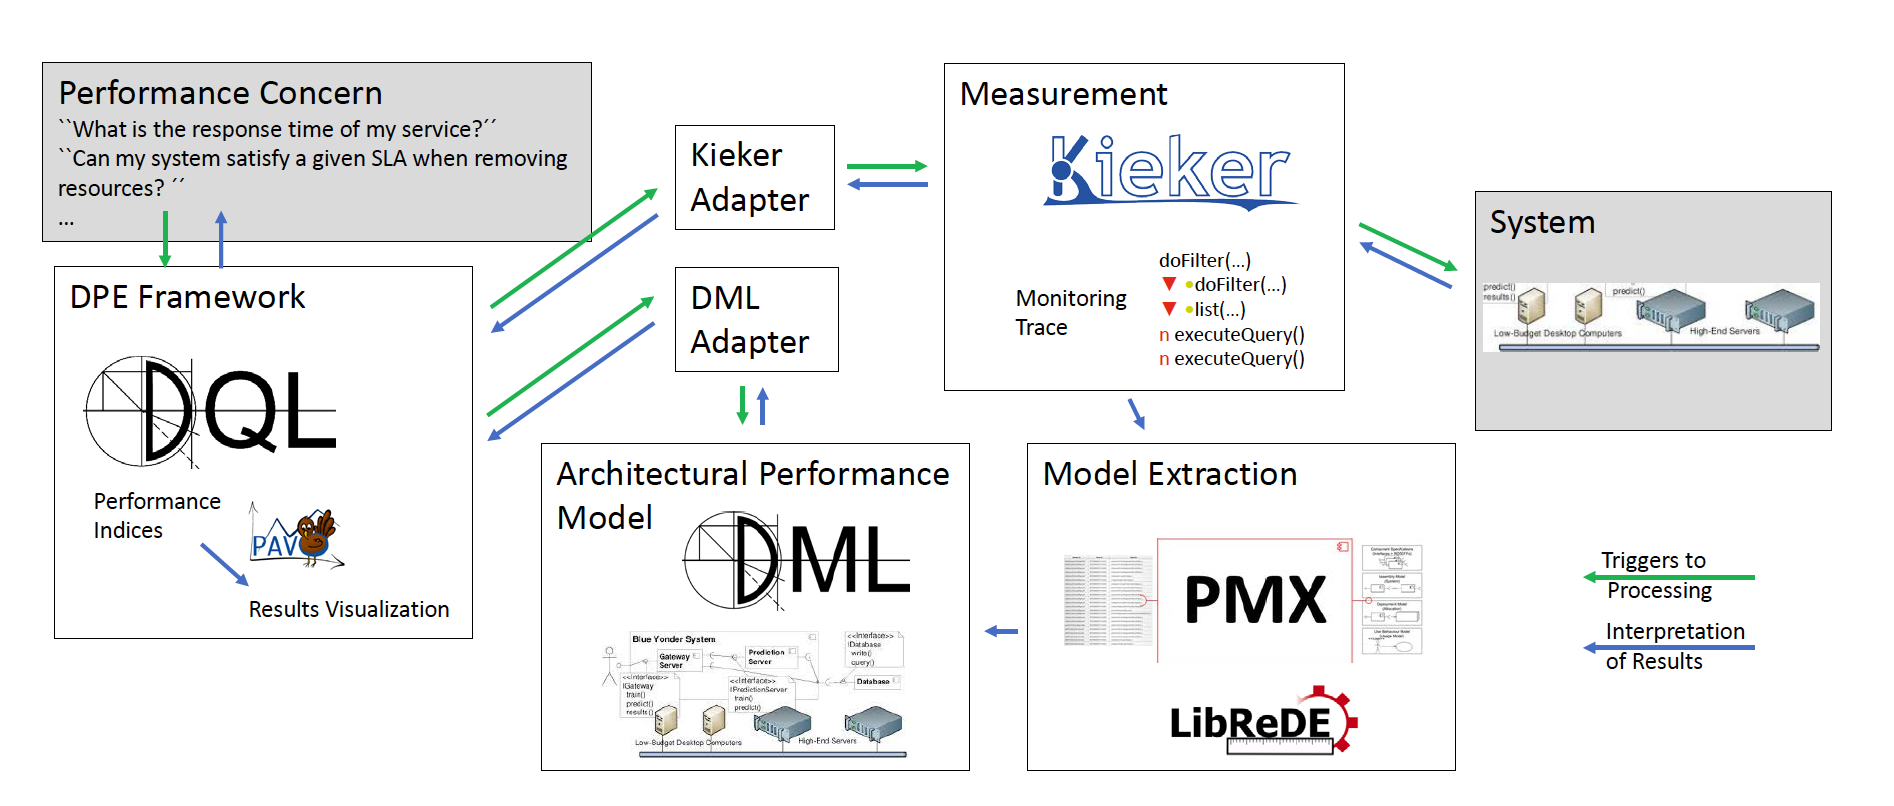
\includegraphics[width=17cm]{declarative-performance-engineering}
  \caption[Herramientas utilizadas para ingeniería de rendimiento declarativo]{Herramientas utilizadas para ingeniería de rendimiento declarativo. Tomado de \cite{Walter:2018:TDP:3185768.3185777}}
  \label{fig:declarative-performance-engineering}
\end{figure}


La figura \ref{fig:declarative-performance-engineering} muestra las herramientas involucradas en el proceso de ingeniería de rendimiento declarativo. Pueden clasificarse en: herramientas para determinar niveles de servicio, para interpretar mediciones obtenidas por medio de la ejecución de un sistema, para extraer modelos de rendimiento y para visualizar resultados. En las figura \ref{fig:declarative-performance-engineering} estas herramientas son:
\begin{itemize}
    \item \textbf{DPE Framework (DPE)}: herramienta para determinar los niveles de servicio de un sistema. Esto lo logra mediante el \emph{Descartes Query Language}(DQL), un lenguaje de consultar indicadores de rendimiento. DPE también incluye \emph{Performance Analysis Visualization} (PAVO) para la visualización de indicadores de rendimiento.
    \item \textbf{Kieker}: una herramienta para el monitoreo del rendimiento de la aplicación (APM por sus siglas en inglés). 
    \item \textbf{Performance Model Extractor (PMX)}: una herramienta que puede derivar modelos de rendimiento a partir de los datos del monitoreo del rendimiento de la aplicación. Puede tomar los datos obtenidos por Kieker y generar modelos de rendimiento en PCM y DML (sección \ref{sec:dml})
\end{itemize}

 
\subsection{Computación en nube}

Según el NIST\cite{Mell:2011:SND:2206223}, el \emph{Cloud Computing}, o la Computación en la Nube, es un modelo que, desde la perspectiva del consumidor, permite el acceso conveniente, por demanda, desde alguna red, a un conjunto de recursos computacionales específicos y configurables (por ejemplo, redes, servidores, almacenamiento, aplicaciones y servicios) que pueden ser rápidamente provisionados y entregados con un esfuerzo mínimo de administración o de interacción con el proveedor del servicio.

\subsubsection{Modelos de entrega de servicio}

La definición del NIST presenta 3 modelos básicos de servicio. Aunque los proveedores de servicios de Cloud han creado muchas variaciones de ofertas \emph{``as-a-Service''}, estos 3 siguen siendo considerados los fundamentales. En la figura \ref{fig:iaas-vs-paas-vs-saas} se muestra lo que se conoce como infraestructura como servicio (IaaS), plataforma como servicio (PaaS) y software como servicio y (SaaS) y las áreas que abarcan en términos de infraestructura, plataforma y software dentro de un esquema de computación en la nube.

\begin{figure}[h]
  \centering
  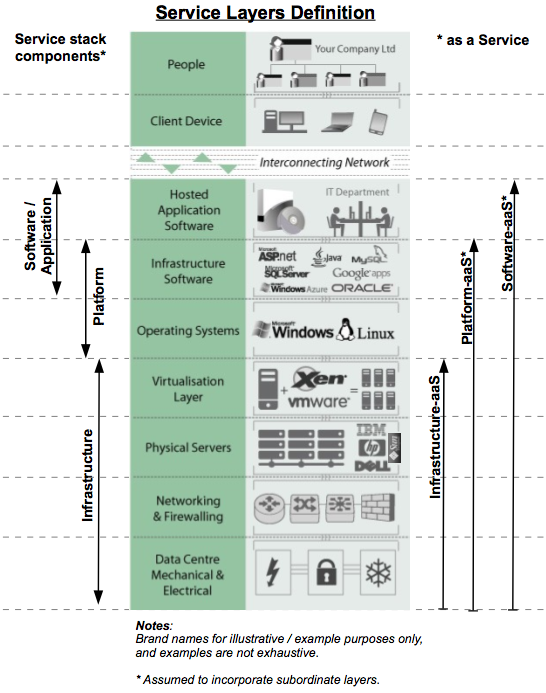
\includegraphics[width=13cm]{Kate-Service-layers-IaaS_PaaS_SaaS}
  \caption[Niveles de servicio presentes en computación en la nube]{Niveles de servicio presentes en computación en la nube. Tomado de \protect\cite{kate-craig}}
  \label{fig:iaas-vs-paas-vs-saas}
\end{figure}


\paragraph{Software como Servicio (SaaS)}
El cliente usa una aplicación, que se ofrece como un servicio accedido remotamente con protocolos estandarizados, pero no controla el sistema operativo, los servidores de aplicación, el hardware o la infraestructura de red en la que opera. El proveedor instala, administra y mantiene el software. El proveedor no necesariamente es dueño de la infraestructura física donde el software se está ejecutando. En general, se puede considerar un servicio para usuarios finales.

\paragraph{Plataforma como Servicio (PaaS)}
El cliente usa un sistema hospedado para sus aplicaciones. El cliente controla las aplicaciones que ejecuta en el ambiente (y posiblemente tenga algún control sobre el ambiente de hospedaje), pero no tiene acceso ni controla el sistema operativo, el hardware o la infraestructura de red donde ellas se ejecutan. La plataforma es típicamente un marco de ejecución aplicativo. El proveedor administra la infraestructura de software de la nube para la plataforma. En este caso, el cliente por lo general es un desarrollador de software.

\paragraph{Infraestructura como Servicio (IaaS)}
El cliente utiliza recursos computacionales fundamentales como poder de procesamiento, almacenamiento, comunicaciones y \emph{middleware}. El cliente puede controlar el sistema operativo, el almacenamiento, implementar aplicaciones y posiblemente algunos componentes de red como cortafuegos (\emph{firewalls}) y balanceadores de carga, pero la infraestructura física de red y de hardware no le pertenece. Los clientes habituales de estos servicios son administradores de sistemas.

\subsubsection{\emph{Serverless y Function-as-a-Service}}
FaaS es un área de lo que hoy se conoce como computación sin servidores o \emph{serverless computing}. Amazon.com, uno de los principales propulsores de esta tendencia define \emph{serverless} como una tecnología la cual permite construir y ejecutar aplicaciones y servicios sin necesidad de pensar en los servidores. Las aplicaciones \emph{serverless} no requieren de aprovisionamiento, escalamiento y administración de ningún servidor. Se puede construir con ella casi cualquier tipo de aplicación o servicio, y todo lo que se requiere para ejecutar y escalar la aplicación con alta disponibilidad es gestionado por el proveedor del servicio\cite{amazon:serverless-definition}. 

FaaS se refiere a un tipo de aplicación \emph{serverless} en donde la lógica del lado del servidor es escrita por un desarrollador pero, a diferencia de arquitecturas tradicionales, esta se ejecuta en contenedores de cómputo que no mantienen estado, son activados por medio de eventos, son efímeros (pueden durar solo una invocación) y son totalmente administrados por un tercero\cite{mike-roberts-serverless}.

Cabe destacar que aunque el término \emph{serverless} ha llegado a ser utilizado para referirse de forma directa a plataformas FaaS, hoy en día las aplicaciones de \emph{serverless computing} abarcan otros tipos de servicios como almacenamiento, mensajería, análisis de datos, seguridad, entre otros.

\subsubsection{Proveedores de servicios de \emph{Function-as-a-Service}} \label{sec:proveedores-faas}

Los principales proveedores de servicios de FaaS son: AWS Lambda, Google Functions, Microsoft Azure Functions e IBM Apache OpenWhisk Functions\cite{novkovic-nemanja}.

\paragraph{AWS Lambda} (\url{https://aws.amazon.com/lambda/}) Proporcionado por Amazon Web Services. Soporta varios lenguajes como NodeJS, Java, C\# y Python. Rango de asignación de memoria: mínimo 128Mb, máximo 1536Mb. Capacidad de disco (espacio en \texttt{/tmp}) 512Mb. La duración máxima de ejecución por solicitud es de 300 segundos.

El precio se establece en \$0.20 por millón de solicitudes y \$0.00001667 por Gigabyte por segundo. 1 millón de solicitudes y 400.000 GBs por mes son gratuitos.

\paragraph{Google Functions} (\url{https://cloud.google.com/functions}) Solamente soporta NodeJS. Está limitado a 1000 funciones con una duración máxima de 540 segundos por cuenta. 
El precio se establece en tres modelos diferentes. El primero es de \$ 0,40 por millón de invocaciones, pero considera que 2 millones de invocaciones son gratuitas. El segundo modelo de precio es de \$0.0000025 por GBs con 400,00 GBs por mes son gratis. El tercer modelo de precios, es de \$0.0000100 GHz por segundo con 200,000 GHz por segundo al mes que son gratuitos.

\paragraph{Microsoft Azure Functions} (\url{https://azure.microsoft.com/en-us/services/functions}) Soporta lenguajes como NodeJS, C\#, F\#, Python, PHP y Java. Azure está limitado a solo diez ejecuciones simultáneas por una función. No hay límites en el límite máximo de tiempo de ejecución. Utiliza dos modelos de precios diferentes. El primero es de \$0.000016 GBs, con 400,000 GBs por mes que son gratuitos. El segundo modelo es de \$0.20 por millón de ejecuciones, con 1 millón de ejecuciones por mes de forma gratuita.

\paragraph{IBM Apache OpenWhisk Functions} (\url{https://www.ibm.com/cloud/functions}) Soporta lenguajes como NodeJS, Swift, Java, PHP, Go y Python. Se puede utilizar cualquier otro lenguaje de programación siempre y cuando de proporcione un contenedor de Docker para esto. Tiene un costo básico que es de \$0.000017 por segundo de ejecución, por GB de memoria asignada.

\paragraph{Otros proveedores de servicios FaaS} Se pueden encontrar otros proveedores y herramientas para utilizar el modelo de funciones en la nube. Entre ellos se encuentran:
\begin{itemize}
    \item Apache OpenWhisk: \url{http://openwhisk.incubator.apache.org/}
    \item Webtask: \url{https://webtask.io/}
    \item OpenFaas: \url{https://github.com/openfaas/faas}
    \item IronFunctions: \url{https://github.com/iron-io/functions}
    \item Kubeless: \url{http://kubeless.io/}
    \item Fn Project: \url{http://fnproject.io/}
    \item Spotinst Functions: \url{https://spotinst.com/products/spotinst-functions/}
\end{itemize}

\newpage

\section{Trabajos relacionados}

\subsubsection{Ingeniería de rendimiento de software en aplicaciones en la nube}

El estilo de arquitectura basado en microservicios es uno de los que ha logrado ganar mayor adopción y popularidad dentro de la comunidad de desarrolladores. Los microservicios, son una arquitectura de software que involucra la construcción y entrega de sistemas que se caracterizan por ser servicios pequeños, granulares, independientes y colaborativos \cite{10.1007/978-3-319-62636-9_11}. Con respecto de SPE y microservicios se reporta que existen muchos retos en investigación que han sido poco o nada abordados. 

En \cite{Heinrich:2017:PEM:3053600.3053653} se planean el monitoreo, pruebas y modelado del rendimiento como las tres áreas en donde se carece de investigación y desarrollo de SPE y microservicios. Se argumenta que aún hacen falta enfoques de SPE que tomen en cuenta las particularidades de los microservicios. Aderaldo et al.\cite{7968049} señala una falta de investigación empírica repetible sobre diseño, desarrollo y evaluación de aplicaciones de microservicios y que esto dificulta la evaluación de este tipo de aplicaciones pues se cuenta con muy pocas aplicaciones y arquitecturas de referencia, así como de cargas de trabajo que contribuyan a caracterizar comportamiento.

El reporte de \cite{DBLP:journals/corr/BrunnertHWDHHHJ15} también proporciona un listado de los retos asociados con microservicios y SPE, haciendo énfasis en actividades de SPE relacionadas con la integración de actividades de desarrollo y de operaciones de puesta en producción y mantenimiento del software. Se argumenta que a pesar del alto nivel de adopción de prácticas de integración continua, entrega continua y DevOps por la comunidad de ingeniería de software, ninguna toma en cuenta aspectos relacionados con el rendimiento. Otros estudios, como el llevado a cabo en \cite{7930195}, indican que uno de los atributos de calidad que ha recibido mayor atención en la investigación en microservicios es el de la eficiencia del rendimiento pero vista mayoritariamente desde el punto de vista de la escalabilidad y mantenibilidad del código de los microservicios y su instalación.


%\textbf{[INCLUIR ESTUDIOS EN DONDE SI SE HA HECHO INVESTIGACION DE SPE Y MICROSERVICIOS?]}

\subsubsection{\emph{Serverless y Function-as-a-Service}}
%FaaS es un área de lo que hoy se conoce como computación sin servidores o \emph{serverless computing}. Amazon.com, uno de los principales propulsores de esta tendencia define \emph{serverless} como una tecnología la cual permite construir y ejecutar aplicaciones y servicios sin necesidad de pensar en los servidores. Las aplicaciones \emph{serverless} no requieren de aprovisionamiento, escalamiento y administración de ningún servidor. Se puede construir con ella casi cualquier tipo de aplicación o servicio, y todo lo que se requiere para ejecutar y escalar la aplicación con alta disponibilidad es gestionado por el proveedor del servicio\cite{amazon:serverless-definition}. 
%
%FaaS se refiere a un tipo de aplicación \emph{serverless} en donde la lógica del lado del servidor es escrita por un desarrollador pero, a diferencia de arquitecturas tradicionales, esta se ejecuta en contenedores de cómputo que no mantienen estado, son activados por medio de eventos, son efímeros (pueden durar solo una invocación) y son totalmente administrados por un tercero\cite{mike-roberts-serverless}.
%
%Cabe destacar que aunque el término \emph{serverless} ha llegado a ser utilizado para referirse de forma directa a plataformas FaaS, hoy en día la aplicaciones de \emph{serverless computing} abarcan otros tipos de servicios como almacenamiento, mensajería, análisis de datos, seguridad, entre otros.

Los investigadores han empezado a describir y analizar FaaS a través de encuestas y experimentos\cite{DBLP:journals/corr/BaldiniCCCFIMMR17,Crane:2017:ESA:3121050.3121086,8360324}, y también por análisis económicos\cite{7515686,8247460}. Sin embargo se reporta que aún no se conoce mucho acerca de SPE en FaaS. En \cite{Heinrich:2017:PEM:3053600.3053653} se menciona que al igual que con microservicios, FaaS también requiere de nuevas estrategias de modelado para capturar el comportamiento del código bajo estas infraestructuras. Los modelos de rendimiento tradicionales basados en la noción de máquinas independientes podría ser inadecuado. 

En van Eyk et al.\cite{vanEyk:2018:SRC:3185768.3186308} se presenta un informe confeccionado por el \emph{Standard Performance Evaluation Corporation RG Cloud Group\footnote{\url{https://research.spec.org/working-groups/rg-cloud.html}}} (SPEC RG Cloud) sobre desafíos asociados a rendimiento en arquitecturas FaaS. Los principales temas son los que tienen que ver con evaluación y comparación de plataformas de FaaS, reducción del \emph{overhead}, políticas de \emph{scheduling}, la relación costo-rendimiento de una función y la predicción del rendimiento. El informe también señala que actualmente muchas de las tareas de evaluación y pruebas para FaaS se vuelven complicadas porque no se cuenta con aplicaciones, arquitecturas ni cargas de trabajo de referencia; este es un trabajo que pretende abordar el SPEC RG Cloud. Con respecto a predicción del rendimiento, se indica que la aplicación de modelos de rendimiento de sistemas de software tradicionales en FaaS trae nuevos retos como la brecha de información (\emph{information gap}) y el rendimiento de una función en particular. La brecha de información significa que el usuario de FaaS no está consciente de los recursos de hardware en los que las funciones son ejecutadas, mientras que, por otro lado, la plataforma de FaaS no tiene información acerca de los detalles de la implementación de la función. Tal y como en las aplicaciones tradicionales, la entrada (tamaño, estructura y contenido) influyen en el rendimiento de una función, el hecho de tener una infraestructura oculta hace necesario encontrar nuevos modelos que logren predecir de forma precisa el rendimiento de una función. Técnicas de modelado desarrolladas para sistemas de software se podrían aprovechar para FaaS, como por ejemplo modelado y simulación de arquitecturas de software basada en componentes. 

La aplicación de \emph{serverless computing} es una área activa de desarrollo. En trabajos previos \cite{7979855,hendrickson2016serverless} se han estudiado arquitecturas alternativas de \emph{serverless computing} con el fin de explotar aspectos de rendimiento o abordar retos técnicos que otras plataformas no han hecho. También se han investigado arquitecturas para recuperación de información\cite{Crane:2017:ESA:3121050.3121086} y \emph{chatbots}\cite{Yan:2016:BCS:3007203.3007217} utilizando plataformas \emph{serverless}. Muchas otras aplicaciones se han venido desarrollando en campos como \emph{Machine Learning}, seguridad, Internet de las cosas, procesamiento de voz, sistemas de archivos, etc, y son solo una muestra del potencial de esta tecnología. Pese a este potencial, también se reporta que aún no se sabe mucho acerca de cuáles herramientas y arquitecturas tecnológicas se usan para producir, instalar y ejecutar funciones\cite{Spillner:2017:PTS:3147213.3149452}. En \cite{8360324} se examinan factores qué pueden influir en el rendimiento de plataformas de \emph{serverless computing}. De acuerdo con esto, se logran identificar cuatro estados de una infraestructura \emph{serverless}: \emph{provider cold}, \emph{VM cold}, \emph{container cold}y \emph{warm}. Además demuestra cómo el rendimiento de los servicios puede llegar a variar hasta 15 veces según estos estados.

\paragraph{Posicionamiento de la investigación con respecto de la literatura consultada}
La investigación que se propone en este documento, pretende dar un aporte al área de ingeniería de rendimiento de software en aplicaciones en la nube. De acuerdo con el material recolectado, se pudo conocer que existe una necesidad por aplicar enfoques de modelado de rendimiento en el desarrollo de sistemas modernos pero que, por otro lado, los esfuerzos que se han llevado a cabo para esto no han logrado ganar popularidad, o bien, no consideran las particularidades de la computación en la nube. Por ejemplo, se reporta que no existen enfoques de modelado de rendimiento para microservicios, el cual es hoy en día, un estilo de arquitectura de software sumamente popular.

Es por esto que se considera que la realización de un estudio exploratorio para determinar los factores que influyen en el rendimiento de una función en la nube, puede brindar nuevo conocimiento sobre cómo aplicar enfoques de ingeniería de rendimiento conocidos a estas aplicaciones y además podría representar un marco de referencia inicial por medio del cual se pueda evaluar la adopción de estas tecnologías \emph{a priori} y fundamentar el planeamiento de capacidades al dimensionar sistemas intensivos en software que vayan a usar microservicios en ambientes en la nube.

%

%
%\chapter{Justificación}
%\label{cap:justificacion}
%\section{Innovación}
Los aspectos más novedosos que se aportan en esta tesis son:
\begin{enumerate}
    \item Proponer un método mediante el cual se pueden obtener estimaciones del rendimiento de una función en la nube
    \item Realizar modelado y simulación basados en componentes para caracterizar el rendimiento de funciones en la nube sobre plataformas FaaS
    \item Proporcionar, a partir de lo anterior, un modelo del rendimiento de una función en la nube    
\end{enumerate}

Con respecto de (1), en \cite{vanEyk:2018:SRC:3185768.3186308} se reporta que la predicción del rendimiento es uno de los principales retos de investigación en plataformas FaaS y que no se cuenta con modelos de rendimiento que consideren las características de FaaS. Esto abre la posibilidad de explorar la aplicabilidad de técnicas conocidas de modelaje de rendimiento en sistemas de software a nuestro dominio de problema. 

(2) El modelado y simulación de arquitecturas de software basadas en componentes, representa una alternativa atractiva para abordar este problema, pues es un enfoque en donde hay una comunidad de investigación y desarrollo activa que ha logrado generar diversos tipos de herramientas para la estimación del rendimiento de sistemas informáticos. 

(3) La obtención de un modelo de rendimiento de una función en la nube (3), representaría un aporte relevante para SPE y FaaS porque significaría que existe una forma por medio de la cual evaluar el comportamiento de una función sin que esta esté necesariamente instalada en una plataforma FaaS y además permitiría que cambios futuros que necesite esa función puedan ser modelados \emph{a priori}, simularlos y obtener predicciones del impacto de los cambios.



\section{Impacto}
En distintos reportes sobre el estado de tecnologías \emph{serverless} en la industria \cite{dzone-cloud-2018,rightscale-2018,digital-ocean-2018,pivotal-june-2018} se señala que la adopción de este tipo de tecnologías va en franco aumento. En \cite{rightscale-2018} se reporta una tasa de crecimiento del 25\% en su adopción con respecto del 2017. Cloud Foundry Foundation \cite{pivotal-june-2018} indica que en el 2017 ``la mayoría'' de sus encuestados no estaban usando tecnologías \emph{serverless} mientras que para el 2018, solamente 43\% \textbf{no} lo estaba haciendo. En el informe anual del estado de tecnologías en la nube de DZone\cite{dzone-cloud-2018} se notó un incremento del 14\% con respecto del 2017 en el uso de tecnologías \emph{serverless}.

Pese a que los niveles de adopción de esta tecnología van en aumento, estos mismos reportes señalan inconvenientes tales como:
\begin{enumerate}
    \item Es necesario depender de los niveles de servicio de un proveedor
    \item Dificultad para monitorear y depurar
    \item Preocupación por parte de los desarrolladores por el ``cómo funciona'' la función en la plataforma FaaS: ¿se estarán asignando los recursos adecuados para mi función en la plataforma FaaS? ¿Cómo y cuándo se hace?
    \item Límites de tiempo de espera: dependiendo del tiempo de ejecución una función en la nube podría llegar a ser cancelada por la propia plataforma FaaS.
\end{enumerate}

Lo anterior refleja que aún existe una especie de ``área gris'' alrededor del uso de las tecnologías \emph{serverless} y en particular funciones en la nube. Esto es lo que van Eyk et al.\cite{vanEyk:2018:SRC:3185768.3186308} llama brecha de la información: el usuario de FaaS no está consciente de los recursos de hardware en los que las funciones son ejecutadas, mientras que por otro lado, la plataforma de FaaS no tiene información acerca de los detalles de la implementación de la función.

Analizar el rendimiento de una función en la nube y obtener un modelo de este contribuiría a tener un mejor entendimiento de esta tecnología y de cómo esta es gestionada por la plataforma FaaS. Esto permitiría a los arquitectos y diseñadores tener mayor control sobre los cambios en una función para que esta no solamente pueda cumplir con los requerimientos de calidad de servicio sino que también, al ser \emph{serverless} un servicio que se cobra por demanda, colaboraría a reducir gastos, ya que una función que tenga un tiempo de ejecución menor generá menores costos por el uso de la plataforma FaaS.

\section{Profundidad}
Para lograr obtener un modelo de rendimiento de una función en la nube se plantean las siguientes actividades:
\begin{itemize}
    \item Diseño e implementación de un caso de uso de referencia de una función en la nube 
    \item Obtención un modelo:
    \begin{itemize}
        \item Realizar pruebas de carga sobre la función en la nube seleccionada
        \item Obtener métricas asociadas al rendimiento a partir de bitácoras de ejecución de la función
        \item Utilizar las métricas obtenidas para suministrarlas como entrada a una herramienta de extracción de modelos de rendimiento. La herramienta generará como resultado un modelo de rendimiento
    \end{itemize}
    \item Diseñar experimentos y ejecutar simulaciones sobre el modelo obtenido, con el fin de validar las estimaciones o determinar si es necesario calibrar el modelo.
    
%     si los resultados obtenidos logran estimaciones adecuadas de la ejecución de la función o si por el contrario se necesita calibrar el modelo.
\end{itemize}

%\subsection{Implementación de un caso de uso de referencia de una función en la nube} 
%Se seleccionará un caso de uso en el cual el uso de una función en la nube haya mostrado ser una solución adecuada. Una vez identificado este caso de uso, se implementará la función y se instalará en una plataforma FaaS.

%\subsection{Obtención de un modelo} 
%Las plataformas FaaS proporcionan bitácoras en donde se registran métricas asociadas a la ejecución de la función en la nube. Se planea entonces ejecutar pruebas sobre la función en la nube bajo diferentes cargas de trabajo y de estar forma poder contar con una bitácora(s) con todas las métricas obtenidas durante el tiempo que tomó la ejecución de las pruebas. 



%
%\chapter{Hipótesis}
%\label{cap:hipotesis}
%En el modelo FaaS, la infraestructura tecnológica subyacente se oculta por completo de los diseñadores y desarrolladores Asimismo, la duración de la ejecución de una función en la nube determina el costo del servicio: entre mayor sea la duración, mayor será el costo. Si bien se han realizado estudios \cite{8360324} para evaluar factores que influyen en el rendimiento de servicios basados en computación \emph{serverless}, el modelado del rendimiento de este tipo de aplicaciones se sigue presentando como un reto de investigación \cite{Heinrich:2017:PEM:3053600.3053653}. El modelado del rendimiento ha ganado considerable atención en la comunidad de ingeniería de rendimiento en las pasadas dos décadas, principalmente en sistemas de software basados en componentes \cite{Koziolek:2010:PEC:1808359.1808729}. Al finalizar y alcanzar los objetivos de la investigación se podrá contar con un marco de referencia que permitirá:
\begin{itemize}
    \item Tener una función en la nube que servirá como prueba de concepto funcional para la evaluación del rendimiento
    \item Contar un método mediante el cual se pueda analizar el rendimiento de una función en la nube por medio de modelado y simulación.
\end{itemize}


Una vez alcanzados los objetivos, será posible responder a la pregunta:


\textbf{¿Es posible estimar el rendimiento de una función en la nube por medio de modelado y simulación basados en componentes?}
%
%\chapter{Objetivos}
%\label{cap:objetivos}
%\section{Objetivo general}
Diseñar un método para modelar el rendimiento de funciones en la nube alojadas en plataformas \emph{Function-as-a-Service} por medio del modelado y la simulación basados en componentes, con el fin de evaluar los factores que pueden influir en su comportamiento. 

\section{Objetivos específicos}
\begin{enumerate}
    \item Revisar el estado del arte de trabajos relacionados con enfoques de predicción y medición del rendimiento en sistemas de software como servicio.
    \item Sintetizar un caso de uso de una función en la nube considerada como de referencia, con el propósito de analizar su comportamiento.
    \item Elaborar, conforme a un diseño experimental, pruebas de rendimiento sobre el caso de uso seleccionado a fin de obtener datos base.
    \item Analizar los datos experimentales mediante herramientas de extracción de modelos de rendimiento de software.
    \item Proponer y validar modelos de rendimiento a partir de los experimentos realizados.        
    \item Formular una guía metodológica para dar a conocer aspectos de rendimiento en funciones en la nube a partir de la experiencia obtenida.
\end{enumerate}
%
%\chapter{Alcance}
%\label{cap:alcance}
%El trabajo propuesto comprende:
\begin{itemize}
    \item El estudio de los factores que pueden influir en el rendimiento de un caso de uso de una función en la nube bajo una plataforma FaaS en particular. Se espera que, a partir de la experiencia generada y los datos recolectados, este trabajo pueda ser replicado con otras funciones en la nube bajo plataformas FaaS alternativas.
    \item La propuesta de un modelo de rendimiento que permita la simulación de la ejecución de una función en la nube y obtener, a partir de esta, estimaciones del tiempo de respuesta de la ejecución de la función.
\end{itemize}


El trabajo propuesto \textbf{no} comprende:
\begin{itemize}
    \item El modelado o simulación de toda una plataforma FaaS.
    \item La realización de un modelo o estudio de los aspectos económicos asociados a la ejecución de una función en la nube.
    \item Estudiar el rendimiento de funciones en la nube que mantengan alguna relación o dependencias entre sí (orquestación de funciones).
    \item Experimentar con múltiples plataformas FaaS ni con diversos lenguajes de programación.
    
\end{itemize}

%
%\chapter{Entregables}
%\label{cap:entregables}
%\section[Revisión de literatura]{Revisión de literatura\\\small{Alineado con objetivo específico 1}}
Se pretende identificar los resultados de otros estudios relacionados con el modelado de rendimiento de software, así como retos y oportunidades de investigación que existan en esta área. Las preguntas de investigación inicialmente propuestas son las siguientes:
\begin{itemize}
    \item[\textbf{PI1}] ¿Cuáles enfoques de predicción y medición del rendimiento en sistemas de software basados en componente se han propuesto?
    \item[\textbf{PI2}] ¿Cuáles enfoques de predicción y medición de rendimiento de software se han utilizado para aplicaciones en la nube?
    \item[\textbf{PI3}] ¿Qué retos y oportunidades existen con estos enfoques en la actualidad?
    \item[\textbf{PI4}] ¿Qué herramientas hay disponibles para el modelado de rendimiento de software?
\end{itemize}

\section[Implementación de caso de uso de función en la nube]{Implementación de un caso de uso de función en la nube\\\small{Alineado con objetivo específico 2}}

Identificar un caso de uso de que sea considerado como de referencia o de utilidad común en donde las funciones en la nube hayan mostrado ser un buenas candidatas para su solución. Se procederá a implementar este caso de uso e instalarlo en una plataforma FaaS. Esta será la función que servirá como base para futuros análisis.

\section[Pruebas sobre el caso de uso]{Pruebas sobre el caso de uso\\\small{Alineado con objetivo específico 3}}

\subsection{Diseño experimental}
Planeamiento y definición de las variables por observar de las pruebas de carga.

\subsection{Pruebas de carga}
Diseño, ejecución y análisis de los resultados de las pruebas.

\newpage

%\subsection{Resultados}


%\section[Medición del rendimiento del caso de uso]{Medición del rendimiento del caso de uso\\\small{Alineado con objetivo específico 3}}
%Al caso de uso identificado se le realizarán mediciones de su rendimiento por medio de diferentes cargas de trabajo. Esto permitirá conocer el comportamiento de la función y utilizar los resultados obtenidos en estas mediciones para contrastar resultados posteriores.

\section[Modelado y análisis del rendimiento de la función]{Modelado y análisis del rendimiento de la función\\\small{Alineado con objetivo específico 4}}
Se tomarán los datos generados por las pruebas anteriores para utilizarlas como entrada y, a partir de ellos, realizar una labor de análisis y modelado.

\section[Modelo de rendimiento de la función en la nube]{Modelo de rendimiento de la función en la nube\\\small{Alineado con objetivo específico 5}}
A partir de la función propuesta, pruebas y análisis del rendimiento por medio de herramientas de modelado, se propondrá un modelo que logre caracterizar el comportamiento de la función.

\subsection[Simulaciones sobre el modelo propuesto]{Simulaciones sobre el modelo propuesto}
Para validar el modelo propuesto, se ejecutarán simulaciones sobre él y de esta forma determinar si los resultados de las simulaciones se corresponden con los obtenidos en las pruebas de rendimiento de la función.

\section[Guía metodológica]{Guía metodológica\\\small{Alineado con objetivo específico 6}}
Una vez realizado el estudio, se estructurará una descripción del método utilizado para estimar el rendimiento de una función en la nube. 
%
%\chapter{Metodología}
%\label{cap:metodologia}
%\section{Etapa 1}
\subsection{Selección de caso de uso}
Uno de los principales problemas de hacer ingeniería de rendimiento para software en la nube es que no existen aplicaciones de referencia que hayan ganado popularidad o cuyo desarrollo se encuentre activo. A pesar de esto y de su reciente adopción, la industria ha empezado a reconocer casos de uso en donde las aplicaciones \emph{serverless} encajan mejor. Amazon Web Services(AWS)\cite{serverless-architecture-patterns} reconoce cinco patrones de uso predominantes en su servicio AWS Lambda:
\begin{enumerate}
    \item Procesamiento de datos dirigidos por eventos.
    \item Aplicaciones Web.
    \item Aplicaciones móviles e Internet las cosas (IoT).
    \item Ecosistemas de aplicaciones \emph{serverless}.
    \item Flujos de trabajo dirigidos por eventos.
\end{enumerate}
 
Uno de las aplicaciones más comunes en \emph{serverless} es desencadenar acciones luego de que ocurre un evento (1), por ejemplo luego de la modificación de un registro en una base de datos o bien luego de que se publica un mensaje en una cola de mensajería. Esto puede provocar que se active una función Lambda\footnote{En la plataforma AWS Lambda } que toma como entrada el evento recién publicado para su posterior procesamiento. Este estilo de caso de uso encaja bien en ambientes híbridos: ambientes en donde tecnologías \emph{serverless} se aprovechan para realizar funciones específicas dentro de una aplicación (o aplicaciones) más grande.

AWS ha publicado una serie de arquitecturas de referencia\cite{aws-lambda-ref-arch} para su plataforma FaaS, AWS Lambda. Dentro de estas arquitecturas se destaca el caso de uso de un manejador de imágenes (\emph{Image Handler})\cite{aws-lambda-image-handler}. 

\begin{figure}[h]
  \centering
  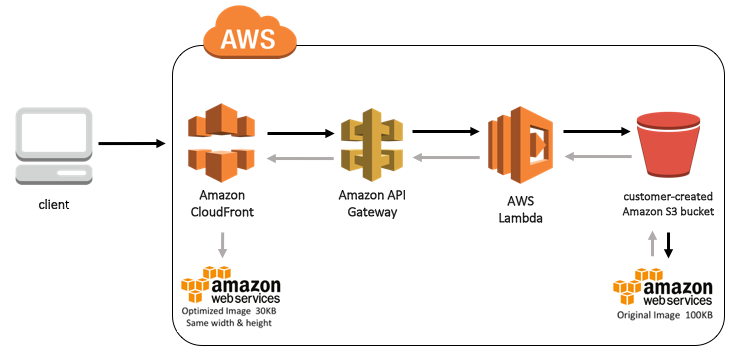
\includegraphics[width=15cm]{serverless-image-handler-architecture}
  \caption[Arquitectura del manejador de imágenes]{Arquitectura del manejador de imágenes. Tomado de \protect\cite{aws-lambda-image-handler}}
  \label{fig:serverless-image-handler-architecture}
\end{figure}

\subsection{\emph{Manejador de imágenes}} \label{sec:manejador-imagenes-1}
Sitios Web con imágenes grandes pueden experimentar tiempos de carga prolongados, es por esto que los desarrolladores proporcionan diferentes versiones de cada imagen para que se acomoden a distintos anchos de banda o diseños de página. Para brindar tiempos de respuesta cortos y disminuir el costo de la optimización, manipulación y procesamiento de las imágenes, AWS propone un manejador de imágenes \emph{serverless}, al cual se le pueda delegar tal trabajo como una función Lambda sobre la plataforma FaaS.


A continuación se describe la arquitectura de la figura \ref{fig:serverless-image-handler-architecture}:
\begin{enumerate}
    \item Amazon CloudFront provee una capa de \emph{cache} para reducir el costo del procesamiento de la imagen
    \item Amazon API Gateway brinda acceso por medio de HTTP a las funciones Lambda
    \item AWS Lambda obtiene la imagen de un repositorio de Amazon Simple Storage Service (Amazon S3) y por medio de la implementación de la función se retorna una versión modificada de la imagen al API Gateway
    \item El API Gateway retorna una nueva imagen a CloudFront para su posterior entrega a los usuarios finales
\end{enumerate}

Cabe mencionar que, en este contexto, una versión modificada de una imagen será cualquier imagen que haya presentado algún tipo de alteración con respeto de una imagen original como, por ejemplo, cambios de tamaño, color, metadatos, etc.

\subsection{Manejador de imágenes para SPE} \label{sec:manejador-imagenes-spe}
Para este estudio se proponemos implementar una variación del manejador de imágenes de la sección \ref{sec:manejador-imagenes-1}, que se muestra en la figura \ref{fig:serverless-image-handler-architecture-spe}.

\begin{figure}[h]
  \centering
  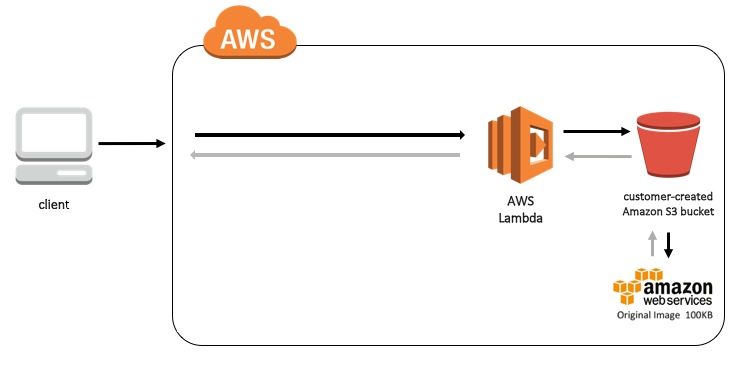
\includegraphics[width=15cm]{serverless-image-handler-architecture-spe}
  \caption[Arquitectura del manejador de imágenes propuesto para el estudio]{Arquitectura del manejador de imágenes propuesto para el estudio.}
  \label{fig:serverless-image-handler-architecture-spe}
\end{figure}

Se han dejado por fuera intencionalmente el AWS CloudFront y el AWS API Gateway. La razón de esto es porque se pretende ejercitar la función Lambda directamente. Se implementará una función Lambda que entregue a partir de una solicitud de redimensionamiento de una imagen almacenada, otra con dimensiones diferentes producida ``al vuelo'' como respuesta a la solicitud. Por ejemplo, si la imagen original mide 500 pixeles de ancho y alto, entregar una con dimensiones de 100 pixeles de ancho y alto. 

Las actividades involucradas en el proceso de redimensionamientos de imágenes se muestran en la figura \ref{fig:serverless-image-handler-architecture-workflow}
\begin{enumerate}
    \item Se envía una solicitud de redimensionamiento de imagen en formato \texttt{JSON} a la función Lambda con los datos acerca de la localización de la imagen y su nuevo tamaño.
    \item La solicitud de redimensionamiento llega a la función Lambda.
    \item La función Lambda solicita al servicio de almacemiento AWS S3 la imagen.
    \item AWS S3 entrega a la función Lambda la imagen solicitada.
    \item La función Lambda inicia el redimensionamiento de la imagen de acuerdo a los parámetros solicitados.
    \item La nueva imagen modificada se entrega al cliente(s).
\end{enumerate}

\begin{figure}[h]
  \centering
  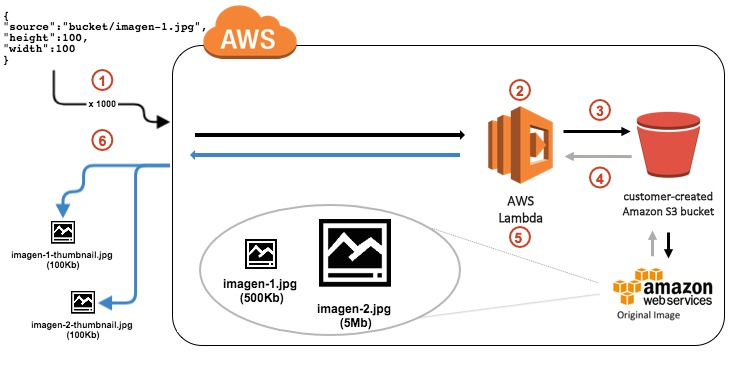
\includegraphics[width=17cm]{serverless-image-handler-architecture-workflow-2}
  \caption[Carga de trabajo sugerida para el manejador de imágenes]{Carga de trabajo sugerida para el manejador de imágenes}
  \label{fig:serverless-image-handler-architecture-workflow}
\end{figure}


A la función Lambda se le realizarán pruebas con imágenes de entrada de distinto tamaño y cargas de trabajo variables para evaluar su comportamiento bajo estos escenarios. Se desea observar el impacto de las pruebas en el tiempo de respuesta de la función. Los resultados obtenidos a partir de estas pruebas van a servir como un punto de referencia para experimentos futuros, como los que se indican en la Sección \ref{sec:experimentos-propuestos}. La figura \ref{fig:serverless-image-handler-architecture-workflow} muestra una sugerencia de dos posibles cargas de trabajo: 

\begin{enumerate}
    \item 1000 solicitudes de cambio de tamaño de una imagen grande. En la figura \ref{fig:serverless-image-handler-architecture-workflow}, \texttt{imagen-2.jpg} de tamaño de 5Mb, representa una imagen grande.
    \item 1000 solicitudes de cambio de tamaño de una imagen pequeña. En la figura \ref{fig:serverless-image-handler-architecture-workflow}, \texttt{imagen-1.jpg} de tamaño menor o igual a 500Kb, representa una imagen pequeña.
\end{enumerate}

En principio las cargas de trabajo generadas serían \emph{cerradas}, lo que quiere decir que una solicitud se ejecuta solamente hasta que la anterior se termina. Esto ayudará en principio a tener mejor trazabilidad de lo que ocurre con la función.

\paragraph{¿Por qué este caso de uso se considera relevante?}
A continuación se listan las características que hacen este caso de uso representativo e interesante:
\begin{itemize}
    \item Sencillo de entender e implementar: se cuenta únicamente con una función la cual lleva a cabo una tarea muy específica.
    \item Popular: sigue un patrón de procesamiento dirigido por eventos y, como se señala en \cite{serverless-architecture-patterns}, este es uno de los más populares que se ha empezado a adoptar para aplicaciones \emph{serverless}. Otra de las razones de la popularidad de este caso de uso es que permite a los desarrolladores crear una unidad de instalación independiente y especializada para el manejo de imágenes, liberando así a sus servidores y aplicaciones del manejo de las peticiones y lógica asociadas a estas.
    \item Replicable en otros proveedores de servicios en la nube: varias de las arquitecturas de referencia para \emph{serverless} propuestas por Amazon, están compuestas por herramientas y servicios muy propios de su plataforma, lo cual hace muy difícil su reproducibilidad utilizando otros proveedores. Aunque en principio este trabajo plantea ser elaborado en la plataforma FaaS de Amazon Web Services, AWS Lambda, otros proveedores de servicios (ver sección \ref{sec:proveedores-faas}) en la nube cuentan con sus propias plataformas de FaaS y de almacenamiento, lo cual permitiría replicar lo aquí propuesto en ellos.
    \item Replicable en los lenguajes de programación soportados por plataformas FaaS: actualmente JavaScript, Java (y lenguajes basados en la \emph{Java Virtual Machine}), Python, C\# y Go son los principales lenguajes de programación soportados por las plataformas FaaS. El caso de uso propuesto, no presenta ningún tipo de característica que lo ate a un lenguaje de programación en particular. En todos ellos se cuentan con bibliotecas para manejo de imágenes tanto de forma nativa como por medio de soluciones de terceros. 
\end{itemize}

\subsection{Experimentos propuestos} \label{sec:experimentos-propuestos}

\paragraph{1. Probar la función en la nube con distintos tamaños de imágenes:} Este es el caso que menciona en la Sección \ref{sec:manejador-imagenes-spe} y se muestra en la figura \ref{fig:serverless-image-handler-architecture-spe}. Se probará la función en la nube con dos imágenes: una de tamaño grande (\textasciitilde 5Mb) y una de tamaño pequeño (\textasciitilde 500Kb). El objetivo es comprobar cómo los distintos tamaños de las imágenes influyen en el tiempo de respuesta de la función.

Intuitivamente, se espera que las imágenes de mayor tamaño tomen más tiempo en ser redimensionadas y que lo contrario suceda con las imágenes de menor tamaño. Los resultados obtenidos brindarán una referencia para saber cómo es que los componentes de software asociados al redimensionamiento de la imagen trabajan y qué posibles mejoras podrían realizarse. 

\paragraph{2. Variar volúmenes de envío por unidad de tiempo:} Se ejercitará la función en la nube con una solicitud de redimensionamiento que se repetirá por un tiempo determinado. Por ejemplo:
\begin{itemize}
    \item Una carga de trabajo \emph{cerrada} de una solicitud de redimensionamiento que se repetirá durante 30 minutos. 
\end{itemize}

El objetivo es observar si los tiempos de respuesta de las solicitudes hechas hacia el final del tiempo de ejecución de la prueba son menores a los tiempos de respuesta de las solicitudes hechas al inicio de la prueba. Esto sugeriría (tal y como se señala en \cite{8360324}) que durante las etapas de ejecución inicial de la prueba la función se encontraría en un estado ``frío'', es decir, su infraestructura subyacente necesita ser aprovisionada, mientras que hacia el final de la prueba la función estaría en un estado ``caliente'', en donde la infraestructura de la función estaría altamente disponible para procesar las solicitudes entrantes. (Presutamente mediante el uso...) 

\paragraph{3. Variar intervalo entre lanzamientos de actividad hacia los servidores}
Es una variante del experimento anterior en donde se desea determinar si hay alguna influencia en de los tiempos de inactividad de una función sobre los tiempos de respuesta u otros comportamientos que la plataforma permita observar.


\paragraph{4. Comparar la función en la nube con la función ejecutándose en SAM CLI}

\emph{Serverless Application Model}\footnote{\url{https://docs.aws.amazon.com/serverless-application-model/index.html}} (SAM CLI) es la solución para ejecución de funciones en la nube desarrollada por Amazon para probar funciones en la nube de manera local, emulando un ambiente similar al que se puede encontrar cuando se ejecuta las funciones en el servicio de AWS Lambda.

Debido a la conveniencia que implica probar las funciones en un ambiente local antes de instalarlas en el proveedor en la nube, se propone tomar como base el experimento 1 para ejecutarlo en SAM CLI con el fin de evaluar si los resultados de su ejecución tienen correlación con los resultados obtenidos del modelado y simulación previos de la función.

\section{Etapa 2}

\subsection{Modelo de rendimiento a partir de la función}
Las cargas de trabajo descritas en la sección \ref{sec:manejador-imagenes-spe} van a alimentar la bitácora de eventos de la función. En AWS el servicio encargado de llevar registro de los eventos que suceden en una función Lambda se llama Amazon CloudWatch\footnote{\url{https://aws.amazon.com/cloudwatch}}. 

Para obtener un modelo a partir del comportamiento de una función, se propone adoptar un enfoque similar al que se plantea en Walter et al. \cite{Walter:2018:TDP:3185768.3185777}, en donde a partir de lo que los autores llaman un \emph{enfoque de ingeniería de rendimiento declarativo} se logra automatizar gran parte del proceso de ingeniería de rendimiento y también explorar, responder y visualizar aspectos concernientes al rendimiento de un sistema. Esto se alcanza gracias a una serie de herramientas desarrolladas por el grupo de ingeniería de software de la Universidad Würzburg de Alemania y que están disponibles en \url{http://descartes.tools}.

\begin{figure}[h]
  \centering
  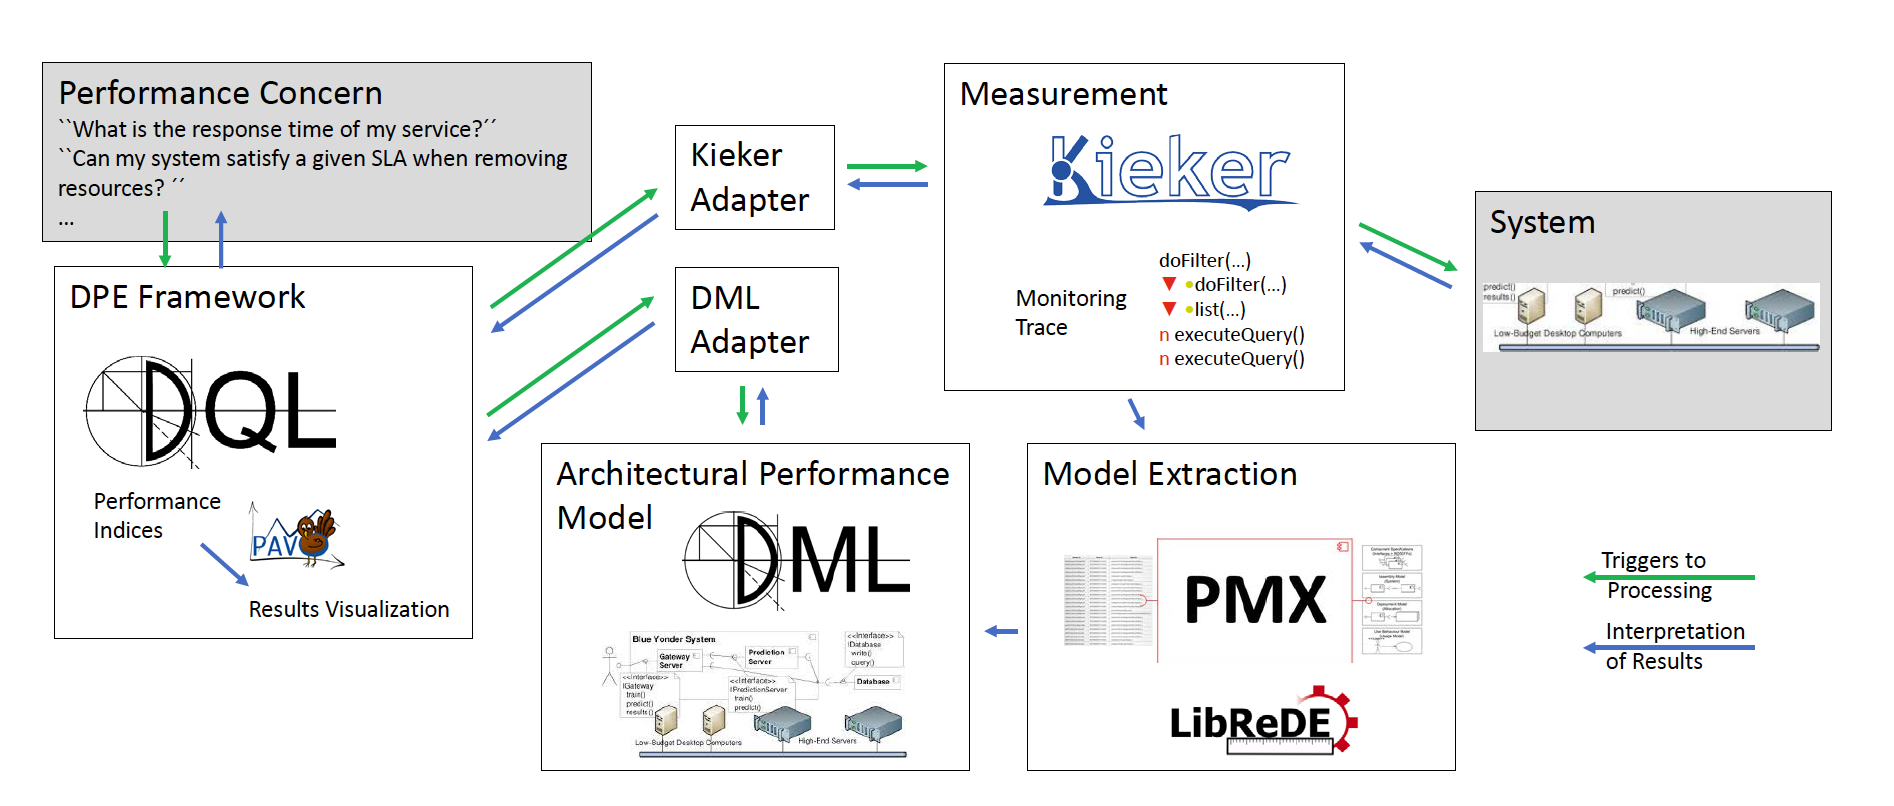
\includegraphics[width=17cm]{declarative-performance-engineering}
  \caption[Herramientas utilizadas para ingeniería de rendimiento declarativo]{Herramientas utilizadas para ingeniería de rendimiento declarativo. Tomado de \cite{Walter:2018:TDP:3185768.3185777}}
  \label{fig:declarative-performance-engineering}
\end{figure}

La figura \ref{fig:declarative-performance-engineering} muestra las herramientas involucradas en el proceso de ingeniería de rendimiento declarativo. Pueden clasificarse en: herramientas para determinar niveles de servicio, para interpretar mediciones obtenidas por medio de la ejecución de un sistema, para extraer modelos de rendimiento y para visualizar resultados. En las figura \ref{fig:declarative-performance-engineering} estas herramientas son:
\begin{itemize}
    \item \textbf{DPE Framework (DPE)}: herramienta para determinar los niveles de servicio de un sistema. Esto lo logra mediante el \emph{Descartes Query Language}(DQL), un lenguaje de consultar indicadores de rendimiento. DPE también incluye \emph{Performance Analysis Visualization} (PAVO) para la visualización de indicadores de rendimiento.
    \item \textbf{Kieker}: una herramienta para el monitoreo del rendimiento de la aplicación (APM por sus siglas en inglés). 
    \item \textbf{Performance Model Extractor (PMX)}: una herramienta que puede derivar modelos de rendimiento a partir de los datos del monitoreo del rendimiento de la aplicación. Puede tomar los datos obtenidos por Kieker y generar modelos de rendimiento en PCM y DML (ver sección \ref{sec:dml})
\end{itemize}

\subsection{Enfoque de trabajo propuesto}
El enfoque que se propone para obtener un modelo de rendimiento a partir de una función, es similar al de Walter et al. \cite{Walter:2018:TDP:3185768.3185777} pero omitimos el uso de las herramientas para determinar y consultar niveles de servicio, y también de visualización. La figura \ref{fig:flujo-de-trabajo-propuesto} muestra los participanes involucrados para lograr esta tarea. 

A partir de las cargas de trabajo a las que fue sometida la función Lambda, métricas de rendimiento serán introducidas dentro del servicio Amazon CloudWatch, este creará la bitácora de la función. Para migrar las métricas de CloudWatch en Kieker, se pretende implementar un adaptador con el fin de tomar una muestra de la bitácora y convertirla a un formato que pueda ser entendido por Kieker. Otra alternativa que se valora es la de publicar las métricas de rendimiento directamente en Kieker  desde la función. 

\begin{figure}[h]
  \centering
  \includegraphics[width=17cm]{flujo-de-trabajo-propuesto-2}
  \caption{Enfoque de trabajo propuesto}
  \label{fig:flujo-de-trabajo-propuesto}
\end{figure}

Una vez que se cuente con una muestra de la ejecución de la función en formato Kieker, esta va a servir como entrada para PMX con el fin de obtener un modelo de rendimiento en PCM. El modelo será utilizado para la ejecución de simulaciones.

\section{Etapa 3: ejecutar simulaciones sobre el modelo obtenido}
\emph{Palladio Workbench}\footnote{\url{https://www.palladio-simulator.com/}} es la herramienta que permite crear y simular modelos basados en PCM. 

Cuando se haya derivado un modelo de rendimiento de la función, se procederá a cargar este modelo en \emph{Palladio Workbench} para modificar y calibrar el modelo y, por medio de las herramientas de simulación que vienen con \emph{Palladio Workbench}, realizar experimentos con el fin de evaluar el grado de coincidencia de los resultados de la simulación con los obtenidos al exponer la función a cargas de trabajo reales.

\addcontentsline{toc}{chapter}{Bibliografía}
\bibliographystyle{ieeetr}
\bibliography{referencias}

\end{document}
%z